% !TEX root = ../These_Robin_Master.tex
\chapter{Explorer visuellement des données de simulation massives pour analyser le comportement d'un modèle.}
\label{chap:chap5}
\begin{center}
{\large Version \hl{2019-05-06}}

\end{center}
\minitoc

%\setcounter{section}{0}
%\clearpage
\section*{Introduction}
\addcontentsline{toc}{section}{\protect\numberline{}Introduction}
%TODO : Ecrire introduction
\hl{A faire}\\
-> Définir notamment la démarche : contraintes générales -> spécificités SimFeodal -> choix méthodos/techniques

%\setcounter{section}{0}
%\clearpage
\section[Capter les sorties de SimFeodal]{{Capter les sorties de SimFeodal}%
	\sectionmark{Capter les sorties}}\label{sec:sorties-simfeodal}
\sectionmark{Capter les sorties}

Pour évaluer un modèle, on s'appuie sur plusieurs indicateurs de sortie de simulation, de types divers (indicateurs numériques, graphiques, cartographiques etc., \hl{cf. chapitre 3, partie théorique}).
Quand le nombre d'indicateurs devient important, comme c'est le cas dans le modèle SimFeodal (chap 3, partie présentation des indicateurs), la consultation des indicateurs pendant le déroulement d'une simulation devient difficile.
La complexité de ces indicateurs augmente dans le cas d'un modèle stochastique comme SimFeodal, où il est nécessaire de multiplier les réplications afin d'avoir une idée fiable des tendances simulées par le modèle.
Le travail de paramétrage d'un modèle requiert de plus de mener différentes expériences, c'est-à-dire de faire varier les paramètres (chap 4) du modèle, démultipliant encore la masse des sorties, et avec elle, la complexité de leur analyse.
Nous détaillons ici les contraintes qu'entraînent ces différentes spécificités des données issues des simulations de SimFeodal.

	\subsection{Masse des données}
	Dans un premier temps, il convient de noter que l'ensemble des indicateurs observés en sortie de SimFeodal reposent sur des données qu'il est nécessaire de produire et d'enregistrer tout au long de la simulation.
	Ainsi, pour pouvoir tracer une courbe de l'évolution du nombre d'agrégats au cours du temps, il faut avoir accès à cette information, et dès lors, enregistrer, à chaque pas de temps, cette valeur dans un fichier numérique adapté.
	Cette information, en tant que telle, est assez faible, aussi bien en valeur sémantique qu'en valeur prise en mémoire.
	Pour autant, on a montré que les indicateurs de sortie étaient nombreux, et avec eux, la quantité de valeurs à stocker augmente.
	Ainsi, à chaque pas de temps, il faudra enregistrer les valeurs de plusieurs variables.
	Cette pratique est habituelle, et un format de données tabulaire se prête bien à un tel enregistrement : une ligne pour chaque pas de temps, et une colonne pour chaque variable à enregistrer.
	On obtiendrait ainsi en sortie de simulation un tableau contenant 18 lignes (le nombre de pas de temps de SimFeodal, cf. \hl{chap2, faire référence à page}) et une cinquantaine de colonnes, ce qui serait assez raisonnable.

	Il faut toutefois prendre en compte un aspect important de l'exploration de données issues de simulations : la production de ces données a un coût temporel important, c'est-à-dire que l'exécution d'une simulation requiert un certain temps (3 à 4 minutes pour une exécution du modèle SimFeodal dans la version présentée dans le \hl{chapitre 2}).
	
	Avec la démultiplication des expériences et la nécessaire évolution du modèle au fur et à mesure de son évolution, il peut être extrêmement difficile, long et fastidieux de ré-exécuter l'ensemble des simulations précédemment effectuées.
	Les indicateurs peuvent évoluer au cours du temps de vie du modèle (cf. \hl{encadré chap 3}), ou plus simplement, on peut être amené à réaliser une observation plus fine des sorties du modèle au fur et à mesure de la calibration de ce dernier.
	Par exemple, parmi les indicateurs de sortie de SimFeodal, on s'intéresse notamment à la composition des pôles, que l'on qualifie assez simplement d'une part avec le nombre d'attracteurs qui les composent, et d'autre part avec l'attractivité qui en résulte.
	À mesure que la calibration du modèle progresse, et si tant est que les indicateurs choisis auparavant ne permettent plus de discriminer certaines variations fines dans les valeurs de paramètres, une étude plus fine du type d'attracteurs composant chaque pôle et de leurs propriétés spécifiques peut aider à discerner des différences entre ces jeux de paramètres et donc à les comparer.
	Cet exemple illustre des ajouts d'indicateurs de sorties, mais, plus pratiquement, on peut aussi être confronté à des modifications des indicateurs existants : le nombre de paroissiens moyen à chaque pas de temps peut être un indicateur utile au départ, mais l'on peut être amené à faire évoluer cet indicateur en une étude de la médiane, ou encore d'un indice de dispersion de la distribution par exemple, parce que la variabilité plus que la moyenne aurait tendance à augmenter au fur et à mesure du paramétrage du modèle.
	On se trouverait alors dans une situation impossible requérant de ré-exécuter les simulations après avoir adapté l'indicateur voulu.
	
	En tenant compte de ces deux éléments, on a tout intérêt à se prémunir de ré-exécutions du modèle, et donc à enregistrer l'état de variables qui ne seraient pas encore mobilisées pour la production d'indicateurs.	
	Dans le cas contraire, pour chaque changement ou ajout d'indicateur, il faudrait relancer des exécutions du modèle sur l'ensemble des jeux de paramètres précédents afin d'être en mesure d'avoir des indicateurs comparables entre les versions.

	Enregistrer l'ensemble des variables d'un modèle est aisé dans le cas d'un modèle théorique simple, par exemple dans le cas d'un modèle comme celui de Schelling \autocite{schelling_dynamic_1971}. Cela se complique quand il s'agit d'enregistrer les variables d'un modèle plus complexe comme SimFeodal.
	Celui-ci comprend en effet bien plus de variables globales, représentant l'état du système dans son ensemble à chaque instant.
	Surtout, SimFeodal est un modèle qui voit interagir plusieurs sortes d'entités, chacune relatives à différents niveaux de granularité spatiale et sociale.
	Afin d'avoir tous les éléments en main une fois la simulation achevée, il est donc nécessaire d'enregistrer l'ensemble des variables non seulement globales, mais aussi afférentes à chacun des types d'agents.
	D'un unique tableau de données exhaustif en sortie du modèle de Schelling, on passe donc à plusieurs tableaux, dont les variables respectives seront propres à chaque type d'agent.

	A ce niveau, l'information en sortie est encore relativement contenue : il y a cinq types d'agents, ayant chacun une douzaine d'attributs, dans SimFeodal. On pourrait donc se contenter de ces cinq tableaux contenant 18 lignes (les pas de temps) et la douzaine d'attributs propres, comme c'est classiquement le cas dans \hl{?}\footnote{
		RC : Trouver exemple de modèle SMA avec plusieurs types d'agents qui ont toutes un intérêt à être examinées spécifiquement, plutôt qu'au moyen d'un indicateur résumé classique (proie-prédateur, nb proies, nb prédateurs par exemple).
	}.

	Reste encore un obstacle majeur à un enregistrement suffisamment exhaustif du déroulement d'une simulation : une part importante des indicateurs s'appuie sur des données individuelles et non agrégées.
	Ainsi, on peut, à chaque pas de temps, enregistrer le nombre de paroisses, leur superficie moyenne ou encore le nombre moyen de paroissiens que chacune dessert.
	Mais cela ne permet en aucun cas d'en dresser une cartographie, c'est-à-dire de réaliser une carte de la localisation et des aires d'attraction des paroisses.
	Cela demanderait, par définition, d'enregistrer la géométrie de chaque paroisse à chaque pas de temps, les configurations spatiales (localisation de chacune et donc distribution spatiale de l'ensemble) variant à chaque simulation.


	Pour faire face à cette situation, on a donc fait le choix, dans SimFeodal, d'enregistrer les états des variables à des niveaux d'agrégation multiples, y compris au niveau de l'agent, à chaque pas de simulation. Dans le cas des paroisses, le volume de données résultant reste contenu : on obtient un tableau d'environ 2000 lignes\footnote{
	Avec une moyenne de 120 paroisses, cela représente $18_{\text{\tiny ~[pas de temps]}} \times 120_{\text{\tiny ~[paroisses]}} \approx 2000$ lignes pour chaque simulation.
	} et une dizaine de colonnes\footnote{
	Les identifiants de la simulation (nom, graine aléatoire), le pas de temps, l'identifiant de la paroisse, puis les différents attributs et la géométrie.
	}.
	L'enregistrement systématique de chaque agent est toutefois bien plus gênant dans le cas d'autres agents, par exemple les foyers paysans. Pour ceux-là, et parce qu'on doit être en mesure d'étudier les liens entre les valeurs de satisfactions et les choix de déplacement, ou encore d'observer la composition précise de la distribution des satisfactions, il est aussi nécessaire d'enregistrer les attributs de chacun d'entre eux. Avec $4000$ foyers paysans à chaque pas de temps, les données changent d'ordre de grandeur\footnote{
	$18_{\text{\tiny ~[pas de temps]}} \times 4000_{\text{\tiny ~[foyers paysans]}} \approx 70~000$ lignes pour une exécution du modèle.
	} : chaque simulation requiert de générer un fichier contenant des dizaines de milliers de lignes, pour un total, pour cet unique fichier, d'une dizaine de mégaoctets occupés.

	A terme, pour enregistrer un état représentatif d'une simulation, c'est-à-dire disposer de suffisamment d'éléments numériques pour pouvoir générer les indicateurs de sortie et prévoir une partie de leur évolution, la masse de données produite est assez conséquente.

	\subsection{Réplications}\label{subsec:capter-replications}

	Comme on l'a vu dans le \hl{chapitre 3}, une simulation ne suffit toutefois pas à évaluer le modèle.
	SimFeodal est ainsi un modèle stochastique, c'est-à-dire qu'une large partie des mécanismes qui l'animent sont basés sur des tirages aléatoires.
	Cet aléa est évident dans les mécanismes faisant appel à un tirage aléatoire explicité, par exemple le choix de déplacement ou non d'un foyer paysan (\hl{cf. chap2, mécanisme déplacement}).
	Dans le cas de ce mécanisme, un foyer paysan mobile se déplacera selon une probabilité dépendant de sa satisfaction.
	Et s'il y a probabilité, il y a donc aléa.
	Même avec une forte satisfaction --- $99\%$ par exemple ---, il reste donc $1\%$ de chance qu'un foyer se déplace, ce qui, sur un grand nombre de tirages (chaque foyer paysan, à chaque pas de temps), aboutit à une probabilité de réalisation non négligeable.
	Et cette probabilité de réalisation sera encore supérieure pour des foyers paysans ayant des niveaux de satisfaction légèrement moindre mais cependant globalement très élevés, supérieurs à $90\%$ par exemple.
	En analysant les sortie du modèle, on aura donc la présence d'\textit{outliers}, qu'il sera important d'isoler, qui présenteront donc des comportements contre-intuitifs puisque résultant d'une probabilité extrêmement faible.
	L'aléa a donc un poids important dans ce type de mécanisme.

	Dans le cas de mécanismes plus anodins, l'aléa est tout de même fortement présent, puisqu'il est au cœur de la conception de SimFeodal.
	Ainsi, le simple ordre dans lequel les agents exécuteront un même mécanisme peut avoir une importance considérable.
	Par exemple, les seigneurs peuvent créer des châteaux, sous condition de puissance (cf. \hl{règle dans chap2}).
	Pour créer ces châteaux, il faut que des agrégats soient disponibles, c'est-à-dire ne comportent pas de château pré-existant à une certaine distance, ce qui devient rapidement le facteur principal de la limitation de l'apparition de châteaux.
	Si un seigneur puissant est souvent appelé en premier pour exécuter ce mécanisme, alors il pourra profiter des nouveaux agrégats disponibles pour créer ses châteaux. Il y aura donc une hiérarchie forte dans le nombre de châteaux possédés par seigneur.
	Au contraire, si l'ordre d'appel des mécanismes favorise des seigneurs différents à chaque pas de temps, alors plus de seigneurs seront en mesure de créer des châteaux, et la hiérarchie sera alors plus faible.
	L'ordre d'exécution, c'est-à-dire l'ordre aléatoire dans lequel les agent sont appelés pour exécuter leurs mécanismes, aura donc un impact important sur les indicateurs de sortie de simulation, sans que cet impact ne puisse être caractérisé au moyen d'indicateurs agrégés.
	Il est ainsi difficile de discerner, dans le comportement du modèle, ce qui relève d'une tendance simulée et ce qui relève de fines variations dues à l'aléa.

	On pourrait objecter qu'en considérant les agents de manière agrégée, donc globale, les probabilités s'effectuent sur suffisamment d'individus pour présenter un résultat cohérent et robuste au niveau de la population dans son ensemble.
	En corollaire, le comportement de chaque agent serait régulé par tant de variables aléatoires qu'on entrerait dans le cadre d'application de la loi forte des grands nombres, les agents adoptant alors en moyenne un comportement proche de l'espérance (moyenne théorique) de chaque tirage.
	Avec ces considérations, on pourrait justifier la robustesse probable des différentes exécutions de SimFeodal.

	SimFeodal n'est toutefois pas simplement un modèle stochastique, mais avant tout, un modèle complexe, c'est-à-dire s'inscrivant dans le champs des systèmes complexes. Sans vouloir ici entrer dans les détails des implications et raisons de ceci, on peut simplement en retenir qu'un modèle tel que SimFeodal est extrêmement sensible aussi bien aux conditions initiales qu'aux différents tirages aléatoires.
	\hl{A développer sérieusement ici, ou bien dans les chapitres 1 ou 2. Il faudra de toute façon faire un point quelque part sur les systèmes complexes, l'émergence etc.}
	Pour illustrer, on peut s'appuyer sur un exemple, caricatural mais possible : à l'initialisation, tous les foyers paysans, placés aléatoirement dans l'espace, seraient concentrés dans un espace d'étendue restreinte.
	Seul un énorme agrégat émergerait donc, et aucun pôle ne serait susceptible dès lors de diviser cet agrégat géant.
	On atteindrait ainsi une situation très éloignée des configurations spatiales observées empiriquement, et très éloignée aussi des réalisations habituelles du modèle.
	En présence d'un seul agrégat, les possibilités de développement d'attracteurs (châteaux et paroisses) pourraient tout aussi bien être fortes que faibles.
	À partir de cette configuration initiale, on ne peut savoir si la situation convergerait vers un agrégat \og paradisiaque\fg{}, extrêmement développé et doté de pôles satisfaisants, ou au contraire, vers un agrégat \og prison \fg{}, où aucun des foyers paysans ne serait satisfait, mais n'aurait non plus d'alternative.
	
	Cet exemple fictif, volontairement caricatural, ne s'est pas présenté jusqu'ici, mais le cas échéant il faudrait pouvoir le repérer, pour éventuellement l'isoler des autres simulations et ne pas le laisser influencer l'analyse d'un jeu de paramètres données.
	De plus, cet exemple concerne uniquement une configuration initiale qui présenterait des caractéristiques tout à fait exceptionnelles.
	Les réalisations aberrantes, soit parce qu'elles seraient issues d'un tirage aléatoire particulièrement défavorable, ou encore parce qu'elles apparaîtraient suite à une succession d'événements improbables qui s'auto-renforceraient, peuvent donc apparaître à toute étape de la simulation, et déformer l'image renvoyée par les tendances simulées par le modèle.
	
	On ne peut donc pas raisonner sur une unique simulation pour évaluer un jeu de paramètres (\hl{cf. chap 3}), mais on ne peut pas non plus se contenter de récupérer le résultat des différentes réplications et d'en tirer une moyenne (selon qu'on s'intéresse par exemple à la tendance générale) ou un écart-type (si l'on cherche justement à observer les variations que peut entraîner l'aléa).

	Pour ces raisons, et pour être en mesure d'embrasser l'entière diversité des sorties de simulations issues de variation de la graine aléatoire, il est donc nécessaire de mener plusieurs réplications de chaque simulation, et d'enregistrer l'entièreté des sorties de simulations dans chacun des cas.
	Le jeu de données produit par une simulation, contenant quelques dizaines de milliers de lignes, est ainsi obligatoirement multiplié par le nombre de réplications.
	Pour l'exploration de SimFeodal, après différents tests, ce nombre a été fixé à $20$ réplications (\hl{J'en aurais sans doute parlé dans le chapitre 3 (évaluation), mais à laisser ici jusqu'à ce que ce soit certain.}).
	La dizaine de mégaoctet issue d'une simulation devient donc approximativement 200 mégaoctets, et le nombre de lignes contenues, par exemple pour les foyers paysans, passe d'à peu près $70~000$ à $1~400~000$\footnote{
	Si cette quantité de données semble tout à fait raisonnable et peut largement être traitée sur un ordinateur classique, on peut toutefois noter qu'elle dépasse toutefois déjà le maximum de lignes ($2^{20}, \approx 1~000~000$) que les tableurs classiques ---
	LibreOffice ou Microsoft Excel dans leurs dernières versions en 2018
	--- sont en capacité de gérer.
	}.

	\subsection{Expériences}\label{subsec:capter-experiences}

	Comme décrit dans le \hl{chapitre 4}, le paramétrage de SimFeodal a demandé plusieurs étapes.
	De plus, chacune de ces étapes représente plusieurs sous-étapes -- les expériences -- faites d'essais et d'erreurs, en faisant varier à chaque fois les valeurs de paramètres de SimFeodal.
	Afin de construire le modèle, puis de l'explorer de manière plus systématique, il a été nécessaire de tester des dizaines de configurations de paramètres.
	Pour comparer, à chaque nouvelle version du modèle, les résultats produits par rapport aux résultats de la version précédente, il est indispensable de conserver, au minimum, l'ensemble des jeux de données de cette version précédente.

	Cet archivage des résultats immédiatement précédents n'est pourtant pas suffisant, pour plusieurs raisons aussi bien éthiques que méthodologiques.
	En premier lieu, pour des impératifs de reproductibilité de la démarche engagée, aussi bien que pour la simple capacité à restituer correctement et rigoureusement les étapes suivies, il fallait conserver l'ensemble des indicateurs de sortie de simulations correspondant à chaque étape ou sous-étape.
	Cette démarche de paramétrage s'inscrivait ainsi sur une durée assez étalée, et suivant un avancement majoritairement non linéaire, fait d'allers-retours, et il était dès lors indispensable de documenter autant que possible chaque étape d'évolution du modèle, et pour cela, de conserver l'ensemble des résultats produits.
	
	Si l'on ajoute les contraintes identifiées précédemment, c'est-à-dire la nécessité de conserver l'ensemble des données brutes plutôt que les seuls indicateurs de sorties, il apparaît qu'on ne peut mener un travail de paramétrage de SimFeodal sans conserver l'ensemble des données produites, c'est-à-dire l'ensemble des attributs de l'ensemble des agents, pour chacun des pas de temps, de chacune des réplications, tout cela pour chacune des expériences.

	En supposant que les 8 étapes présentées dans le chapitre précédent (\hl{ref chap4, étapes}) soient ne serait-ce que constituées de 3 sous-étapes chacune --- ce qui est bien en deçà de la réalité ---, on obtient 24 jeux de paramètres à stocker, puis à devoir mobiliser.
	Cela représente une somme considérable de données (voir \cref{tbl:hierarchie-simulations}), qui se chiffrent en dizaines de millions d'enregistrement\footnote{
	$18_{\text{\tiny ~[pas de temps]}} \times 4000_{\text{\tiny ~[foyers paysans]}} \times 20_{\text{\tiny ~[réplications]}} \times 24_{\text{\tiny ~[jeux de paramètres]}} \approx 35~000~000$ de lignes enregistrées pour les seuls foyers paysans.
	}.
	Si cela ne représente jamais que quelques gigaoctets de données, ce que quiconque a désormais l'habitude de manipuler dans un cadre personnel, en terme de traitement, cette masse de données est à la limite de ce que l'on peut traiter sur un ordinateur individuel.
	Ainsi, selon une approximation courante, on ne peut charger en mémoire de données d'une taille supérieure à la moitié de la mémoire vive disponible, sans même prendre en compte les autres éventuels processus en cours.
	Avec 5 Go de données , il faut donc disposer d'un ordinateur personnel possédant au moins une douzaine de gigaoctets de mémoire vive, et encore, au prix d'un traitement extrêmement lent et bloquant.

	Et encore, on ne mentionne ici que les expérimentations issues des étapes de paramétrage.
	Les phases suivantes d'exploration du comportement du modèle, par exemple relatives à l'analyse de sensibilité du modèle ou à sa calibration, demandent ainsi d'exécuter, et donc d'enregistrer, une masse bien plus importante de simulations.

	\subsection{Des données aux indicateurs}\label{subsec:donnees-indicateurs}
	
	Dans l'ensemble, l'enregistrement et la sauvegarde des données issues de simulations constituent, pour les modèles de simulations basés sur de nombreux agents et mécanismes, une contrainte importante vis-à-vis de l'exploration du comportement de ces modèles.
	
	C'est particulièrement le cas pour SimFeodal, où l'on ne peut se contenter de produire à la volée les indicateurs, pour des raisons de reproductibilité théorique et pratique\footnote{
	\hl{La reproductibilité sera abordée \og longuement\fg{} dans le chapitre 1 (positionnement).}
	}. 

	\begin{table}[!ht]
	\raggedleft
	\resizebox{.85\textwidth}{!}{%
		\begin{tabular}{N|M{2.5cm}|M{2.5cm}|M{2cm}|M{3.5cm}|M{4.5cm}|N|}
			\hline
			&	& \multicolumn{2}{|c|}{\thead{Données}} & \multicolumn{2}{|c|}{\thead{Indicateurs}} \\ \hline
			& \thead{Intitulé} & \thead{Quantité} & \thead{Poids} & \thead{Type} & \thead{Quantité} & \\[25pt] \hline
			\tikzmark{a}& Une simulation & \makecell{$\approx 10^5$ lignes}& $\approx 10$ Mo & \begin{tabular}[c]{@{}l@{}}Visualisations\\ en direct\end{tabular} & \makecell{$\approx 10$ indicateurs}  & \\[50pt] \hline
			\tikzmark{b}& Une expérience & \makecell{$\approx 10^6$ lignes} & $\approx 200$ Mo & Indicateurs de sortie & \makecell{$\approx 30$ indicateurs\\(variabilité des\\réplications)} & \\[50pt] \hline
			\tikzmark{c} & \makecell{Huit étapes\\de\\paramétrage} & \makecell{$\approx ~10^7$ lignes} & $\approx 5$ Go & Indicateurs de sortie & \makecell{$\approx 700$ indicateurs\\ (à comparer entre\\les expériences)} & \\[50pt] \hline
		\end{tabular}%
		\tikz[overlay,remember picture] \draw[->, >=latex', bend right=90, thick, dashed] (a.west) to node[pos=.5, left, align=center, xshift=0pt]{$\times 20$\\$\textrm{réplications}$} (b.west) ;
		\tikz[overlay,remember picture] \draw[->, >=latex', bend right=90, thick, dashed] (b.west) to node[pos=.5, left, align=center, xshift=0pt]{$\times \approx 24$\\$\textrm{expériences}$} (c.west) ;
	}
	\caption{Synthèse de la multiplication des données et indicateurs selon la hiérarchie des simulations.}
	\label{tbl:hierarchie-simulations}
\end{table}
	
	\paragraph*{Analyser une masse de données}
	La masse de données en sortie est impressionnante et requiert dès lors, d'un point de vue technique, d'utiliser des outils adaptés à la manipulation de grands jeux de données.
	Cela exclut de fait l'outillage traditionnel de la géographie quantitative, ne laissant par exemple pas la possibilité d'utiliser les outils à interface graphique classiques.
	Au contraire, face à des données de cet ordre, seules des solutions statistiques, basées sur des analyses en ligne de commande, peuvent être mobilisées.
	Ces solutions doivent en plus être appuyées par des capacités de calculs importantes, sans toutefois justifier encore l'usage de technologies de calcul intensif (\og \textit{High-Performance Computing}\fg{} --HPC --, mobilisé pour l'étude de données plus massives, i.e. trop importantes pour être analysées sur un unique ordinateur ou serveur).
	Cela pose une contrainte dans l'accessibilité aux analyses : le traitement des données requiert des compétences spécifiques en analyse de données volumineuses.
	Dans un contexte interdisciplinaire caractérisé par une large hétérogénéité en matière de pratiques quantitatives, il n'est pas possible de se contenter d'envoyer les jeux de données produits aux thématiciens -- qui ne disposent pas de ces compétences -- : ils seraient alors en difficulté pour en tirer les analyses nécessaire à leur interprétation.

	\paragraph*{Analyser une masse d'indicateurs}
	D'un point de vue thématique, et c'est là l'objectif, cette masse de données doit servir à la production d'indicateurs, nombreux et divers aussi bien dans leur forme que dans les caractéristiques des processus qu'ils décrivent (\hl{ref. chap. 3, indicateurs}).
	Les mêmes raisonnement que pour les données s'appliquent ainsi aux indicateurs.
	Si on peut prendre en compte la variabilité des réplications directement dans les indicateurs produits (par exemple avec des représentations graphiques de type \textit{box-plot} qu'adoptent une forte partie des indicateurs), ce n'est ni possible ni souhaitable entre les différentes expériences.
	De fait, chaque expérience doit pouvoir être comparée aux précédentes sur la base de leurs seules réplications respectives.
	Dès lors, la raison d'être des indicateurs de sortie est de rendre possible une comparaison, indicateur par indicateur, entre chacune des expériences.
	Il est donc indispensable de générer, pour chaque expérience, l'ensemble des indicateurs. En ne considérant ici encore que 24 expériences, cela fait donc déjà plusieurs centaines\footnote{
	En considérant ainsi une trentaine d'indicateurs, on obtient donc $30{\text{\tiny ~[indicateurs]}} \times 24_{\text{\tiny ~[jeux de paramètres]}} \approx 700$ indicateurs uniques.
	} d'indicateurs (\cref{tbl:hierarchie-simulations}).

	Le choix ayant été fait de mener une comparaison visuelle (\hl{ref. dans chapitre 3 : indicateurs uniques vs fonctions objectifs}), on imagine dès lors que celle-ci va être difficile en présence de tant d'indicateurs.

	En sus de la contrainte de l'enregistrement et de la production des indicateurs, le verrou majeur à la compréhension des phénomènes modélisés dans SimFeodal est donc la simple capacité à visualiser et à explorer l'ensemble des indicateurs de sortie.
	Ce qui doit de plus être rendu accessible y compris pour un auditoire non habitué à la manipulation de nombreuses données et sorties quantitatives.


\setcounter{section}{1}
\clearpage
\section[Comment explorer les sorties de SimFeodal ?]{Comment explorer les sorties de SimFeodal ?%
\sectionmark{Explorer les sorties}}\label{sec:explorer-sorties-simfeodal}

	Pour évaluer, de manière approfondie, une expérience (voir \cref{tbl:hierarchie-simulations}) d'un modèle tel que SimFeodal, il est nécessaire de passer en revue de nombreux indicateurs de sortie de simulation.
	Cette évaluation ne vise pas à produire une \og note\fg{} unique et synthétique, mais plutôt à tester la capacité de l'expérience à reproduire les dynamiques que le modèle chercher à reproduire.
	Il ne s'agit pas, à proprement parler, d'une validation du modèle, au sens quantitatif où on pourrait l'entendre.
	On vise plutôt à explorer le comportement du modèle en fonction des mécanismes et valeurs de paramètres choisis.
	Cela aboutit donc sur un jugement qualitatif sur la capacité du modèle à reproduire les dynamiques souhaitées.
	Pour mener cette exploration, il convient d'utiliser des outils adaptés, c'est-à-dire de disposer de solutions techniques permettant le calcul et l'affichage des indicateurs à partir des données produites par le modèle.
	
	Dans le travail mené autour de SimFeodal, plusieurs solutions ont été utilisées au cours des différentes étapes de construction du modèle.
	La restitution purement chronologique de ces solutions ne revêt pas d'intérêt propre, mais les contraintes accumulées au cours de la construction du modèle ainsi que les choix devant permettre de les dépasser nous paraissent très largement génériques et généralisables.
	
	La succession de choix d'outils d'explorations se justifie par les verrous dans l'exploration que chacun de ces outils a permis de débloquer.
	Cela dresse par là-même un portrait des solutions méthodologiques d'exploration de données de simulations dont on peut faire usage selon les contraintes générales des modèles.

	\subsection{Observation en direct ou \textit{a posteriori}}\label{subsec:observation-a-posteriori}

	Classiquement, le premier réflexe d'un modélisateur, du moins pour les modèles à base d'agents, est de définir des sorties graphiques pour accompagner son modèle.
	Les différentes plate-formes de modélisation agent mettent d'ailleurs régulièrement en avant les possibilités de représentations qu'offrent leurs environnements\footnote{
		Voir par exemple les collections de visualisations sur les pages d'accueil de Gama (\href{https://gama-platform.github.io/}{https://gama-platform.github.io/}), de NetLogo (\href{https://ccl.northwestern.edu/netlogo/}{https://ccl.northwestern.edu/netlogo/}), de GeoMASON (\href{https://cs.gmu.edu/~eclab/projects/mason/extensions/geomason/}{https://cs.gmu.edu/$\sim$eclab/projects/mason/extensions/geomason/}) ou encore de Repast (\href{https://repast.github.io/screenshots.html}{https://repast.github.io/screenshots.html}).
	}.
	Visualiser le déroulement d'un modèle \og en direct\fg{} (\og \textit{online}\fg{} dans \cite{grignard_agent-based_2017}), c'est-à-dire au sein de la plate-forme de simulation et au cours l'exécution du modèle, offre ainsi de nombreux avantages : évaluation visuelle du niveau de ségrégation (et de son évolution) dans une implémentation du modèle de Schelling ; visualisation de cohérence du déplacement des nuées d'oiseaux dans un modèle de type \og Flocks\fg{} \autocite{reynolds_flocks_1987} ; ou encore suivi d'un indicateur dans le temps -- la quantité de ressources collectées -- dans un modèle de type \og Sugarscape\fg{} \autocite{epstein_growing_1996}.
	
	Il est à noter que dans le cadre du développement d'un modèle de simulation, l'implémentation du modèle et de son interface graphique sont étroitement liées.
	D'une part, la plateforme de modélisation choisie contraint fortement le type et la diversité des représentations.
	Gama et GeoMASON, par exemple, proposent des modes de visualisation de données géographiques bien plus avancés que NetLogo ou Repast.
	L'interface graphique développée pour chaque modèle est donc largement influencée par la plateforme de simulation dans laquelle il est exprimé.
	D'autre part, dans la plupart de ces plateformes de simulation, l'interface graphique est implémentée au même niveau que le code-source du modèle en lui-même.
	Dans Netlogo et Gama par exemple, l'interface graphique est programmée directement dans le modèle en lui-même, en se basant sur les variables qui y sont déclarées.
	Il n'est donc pas possible de créer une interface graphique générique au sein des plateformes de simulation, laquelle pourrait s'appliquer à plusieurs modèles différents.
	Il est nécessaire, pour chaque modèle, de reconstruire l'interface depuis les briques de bases proposées par les plateformes, c'est-à-dire un ensemble de primitives graphiques permettant de composer une interface intégrée au modèle.

	Dans l'exploration de SimFeodal, la création en direct de quelques graphiques correspondant à des indicateurs étudiés permet d'assurer un rôle de filtrage, grossier, à l'exécution d'une expérience, c'est-à-dire de l'ensemble des réplications nécessaires à son évaluation.
	Après une modification du code-source du modèle, et avant de lancer de nombreuses simulations, on exécute quelques simulations \og manuellement\fg{}.
	On s'assure alors, en direct, que les indicateurs affichés ne présentent pas de caractères aberrants.
	Cela permet de vérifier, avant de lancer des calculs plus conséquents, que le déroulement de la simulation semble cohérent, c'est-à-dire, le plus souvent pour des modifications mineurs du modèle,  qu'un \textit{bug} n'a pas été introduit involontairement.
	
	Le recours à ce type de visualisation en direct des simulations ne peut toutefois être généralisé, c'est-à-dire sorti de son rôle de pré-filtre, en raison de deux principales contraintes.

	La première contrainte, déjà évoquée plus haut, est que le modèle SimFeodal est fortement stochastique.
	Dès lors, la visualisation des indicateurs d'une simulation particulière n'est pas suffisante pour estimer le comportement du modèle.
	En conséquence, les indicateurs choisis pour l'évaluation de SimFeodal prennent presque tous en compte la variabilité des résultats induite par l'exécution de réplications.
	Certains environnements techniques\footnote{
	Gama dans sa dernière version (1.8) par exemple, voir\\ \href{https://gama-platform.github.io/wiki/RunSeveralSimulations.html}{https://gama-platform.github.io/wiki/RunSeveralSimulations.html}.
	} permettent toutefois de mener concomitamment plusieurs réplications d'un même modèle et de visualiser directement pendant l'exécution les résultats agrégés des réplications.
	Cette première contrainte, liée au besoin d'analyser des réplications plutôt que des exécutions isolées, peut donc être dépassée en adaptant l'implémentation du modèle pour faire usage de ces capacités de multi-simulation.

	La seconde contrainte est cruciale dans le cas de SimFeodal et invalide l'usage des méthodes de visualisation en direct.
	On l'a vu, l'exploration des sorties de simulation du modèle repose sur la consultation systématique de plusieurs indicateurs, dont le nombre peut se révéler important pour une analyse approfondie.
	
	Tout d'abord, il est concrètement difficile de représenter tous ces indicateurs au sein de l'interface graphique d'une plate-forme de simulation agent, comme on peut le remarquer, par exemple en \cref{fig:simfeodal_gui_indicateurs} : l'espace occupé par les quelques indicateurs temporels et numériques affichés est déjà important et rend l'interface d'ensemble complexe.
	De plus, et c'est sans doute le verrou majeur, la temporalité de l'exécution d'une simulation -- ou même des réplications nécessaires -- est bien plus courte que celle requise pour la compréhension des résultats produits.
	Une simulation requiert ainsi au maximum quelques minutes.
	Pour pouvoir examiner tous les indicateurs pendant cette durée, il serait nécessaire de mettre la simulation en pause régulièrement, presque à chaque pas de temps.
	On disposerait alors d'un temps suffisant pour observer les indicateurs (organisés en onglets dans l'interface visible dans la \cref{fig:simfeodal_gui_indicateurs}).
	L'analyse des indicateurs de sortie de simulation demandent en effet un examen approfondi, et non simplement superficiel, pour pouvoir juger de l'adéquation de ce que ces indicateurs représentent vis-à-vis des attentes thématiques.
	
	Cette contrainte est renforcée par la pratique d'évaluation que la plupart des chercheurs mobilise.
	L'évaluation n'est pas une étape unique et finie, il est utile de pouvoir revenir sur les résultats à différents moments.
	Cela est par exemple nécessaire quand il s'agit de comparer de nouveaux résultats produits à ceux générés par des expérimentations antérieures.
	On ne peut alors se contenter d'évaluations en direct, même en y consacrant un temps important, simplement parce que par nature, ces évaluations seront à reproduire en plusieurs occasions, et qu'il ne serait alors pas rationnel de relancer, à chaque fois, de nouvelles simulations correspondant à des configurations de paramètres et de mécanismes déjà éprouvées.
	
	Un dernier élément contribue à la difficulté de se baser sur une évaluation en direct : en plus du chercheur, amené à revenir de multiples fois sur les résultats d'une expérience, un modèle co-construit peut être évalué par plusieurs chercheurs différents.
	C'est d'autant plus fréquent en situation d'interdisciplinarité, où les points de vue de chacun des membres sont complémentaires et nécessaires.
	Sauf à faire preuve d'une discipline exacerbée, par exemple en réalisant l'ensemble du travail d'évaluation uniquement en séances de travail simultanées et collectives, l'évaluation par plusieurs personne demande que chacun puisse mener ces analyses selon ses propres temporalités.
	En choisissant de baser l'évaluation d'un modèle uniquement sur une analyse en direct, il faudrait alors que chaque chercheur, à chaque fois qu'il souhaite évaluer une même expérience, ré-exécute le modèle de nombreuses fois.
	Cela serait naturellement possible, mais constituerait clairement un gâchis certain de ressources.
	
	L'évaluation d'un modèle interdisciplinaire et exploratoire ne peut donc que difficilement être réalisé en direct, qui plus est quand elle demande de faire appel, dans un cadre de co-construction, à plusieurs points de vue hétérogènes.
	Les modalités mêmes de l'exploration des sorties d'un modèle à évaluation visuelle requièrent donc que les indicateurs soient visibles et explorables à des temporalités différentes, par des chercheurs différents, depuis des lieux divers.
	
	Il est donc indispensable que les indicateurs soient enregistrés et consultables simplement à tout moment, ce qui élimine de fait la visualisation des indicateurs en direct pendant l'exécution des simulations comme unique méthode d'exploration du comportement des modèles exploratoires et descriptifs.
	
	
	\begin{figure}[H]
		\captionsetup{width=\linewidth}
		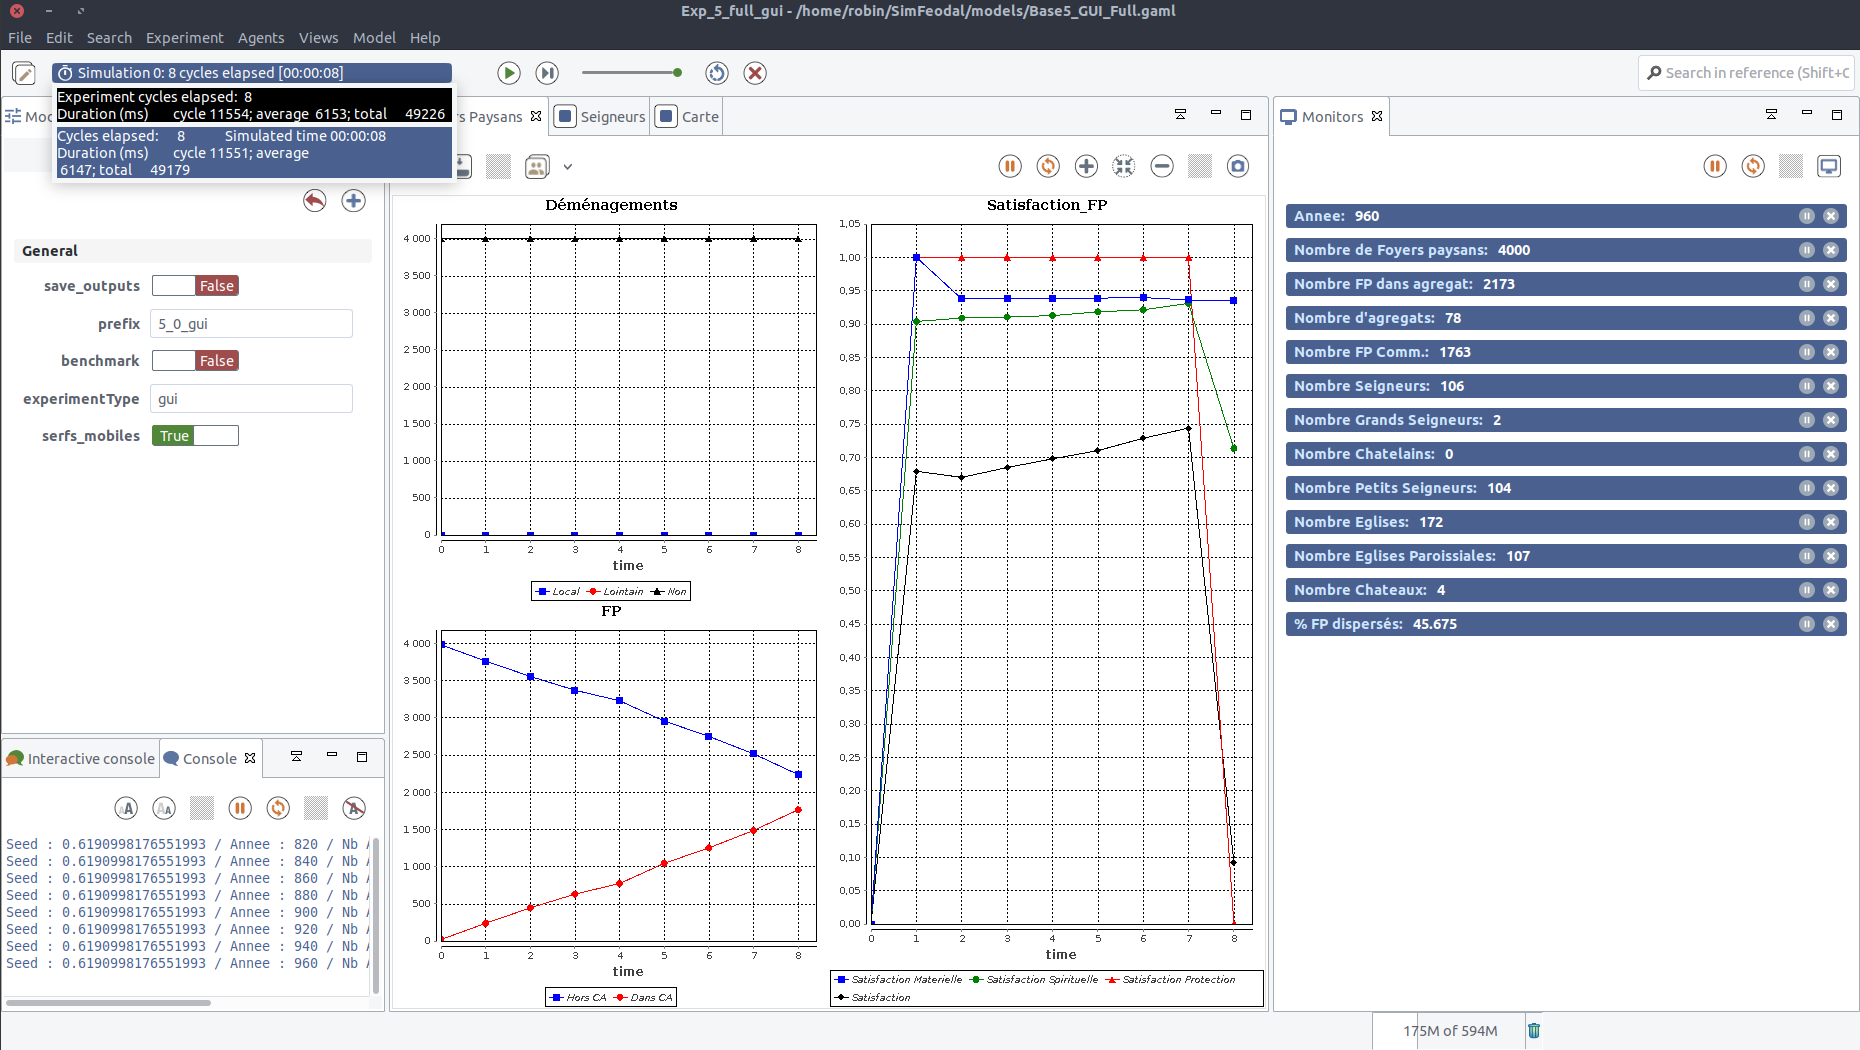
\includegraphics[width=\linewidth]{img/SimFeodal_GUI_FP.png}
		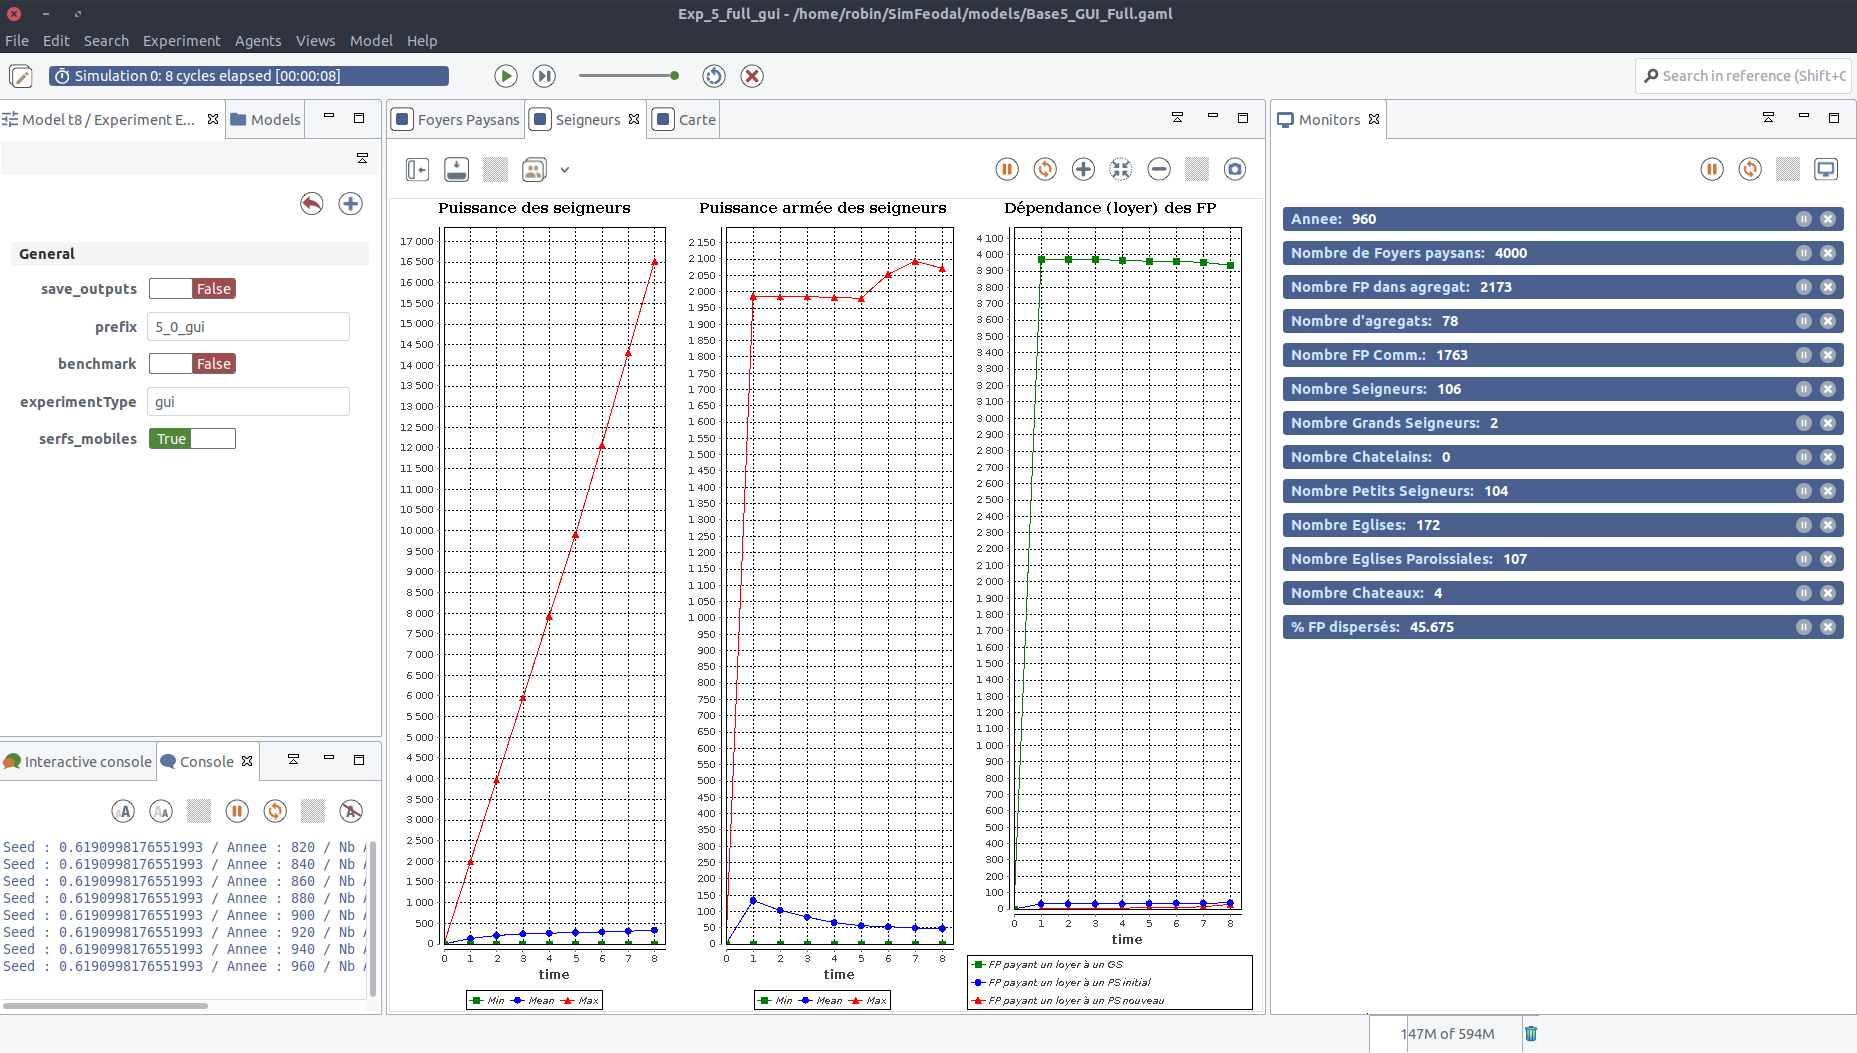
\includegraphics[width=\linewidth]{img/SimFeodal_GUI_seigneurs.png}
		\caption{Indicateurs intégrés à l'interface graphique interne de SimFeodal.
		Dans ces captures d'écrans, il s'agit d'indicateurs liés aux foyers paysans et aux seigneurs.}
		\label{fig:simfeodal_gui_indicateurs}
	\end{figure}
	
	La visualisation en direct n'est donc pas mobilisable en tant que méthode d'évaluation principale, mais elle peut tout de même, comme dans un usage très classique, être utilisée comme un outil de validation interne pour tester chaque modification dans les valeurs de paramètres, remplissant alors le rôle de \og préfiltre\fg{} décrit auparavant.
	Visualiser une seule simulation, avant d'en exécuter les réplications nécessaires, permet ainsi déjà de vérifier que les modifications apportées dans les valeurs de paramètre ou dans les mécanismes n'ont pas entraîné l'apparition de \textit{bugs} ou d'incohérences immédiatement visibles.

	Nous avons donc choisi de développer une interface graphique, très sommaire mais permettant des allers-retours rapides entre l'implémentation et l'exécution, au sein de l'implémentation de SimFeodal.
	Cette interface n'affiche qu'un nombre réduit d'indicateurs (\autoref{fig:simfeodal_gui_indicateurs}), ainsi qu'une représentation cartographique (\autoref{fig:simfeodal_gui_carte}) utile à une analyse rapide du comportement d'ensemble du modèle.

\begin{figure}[H]
	\captionsetup{width=\linewidth}
	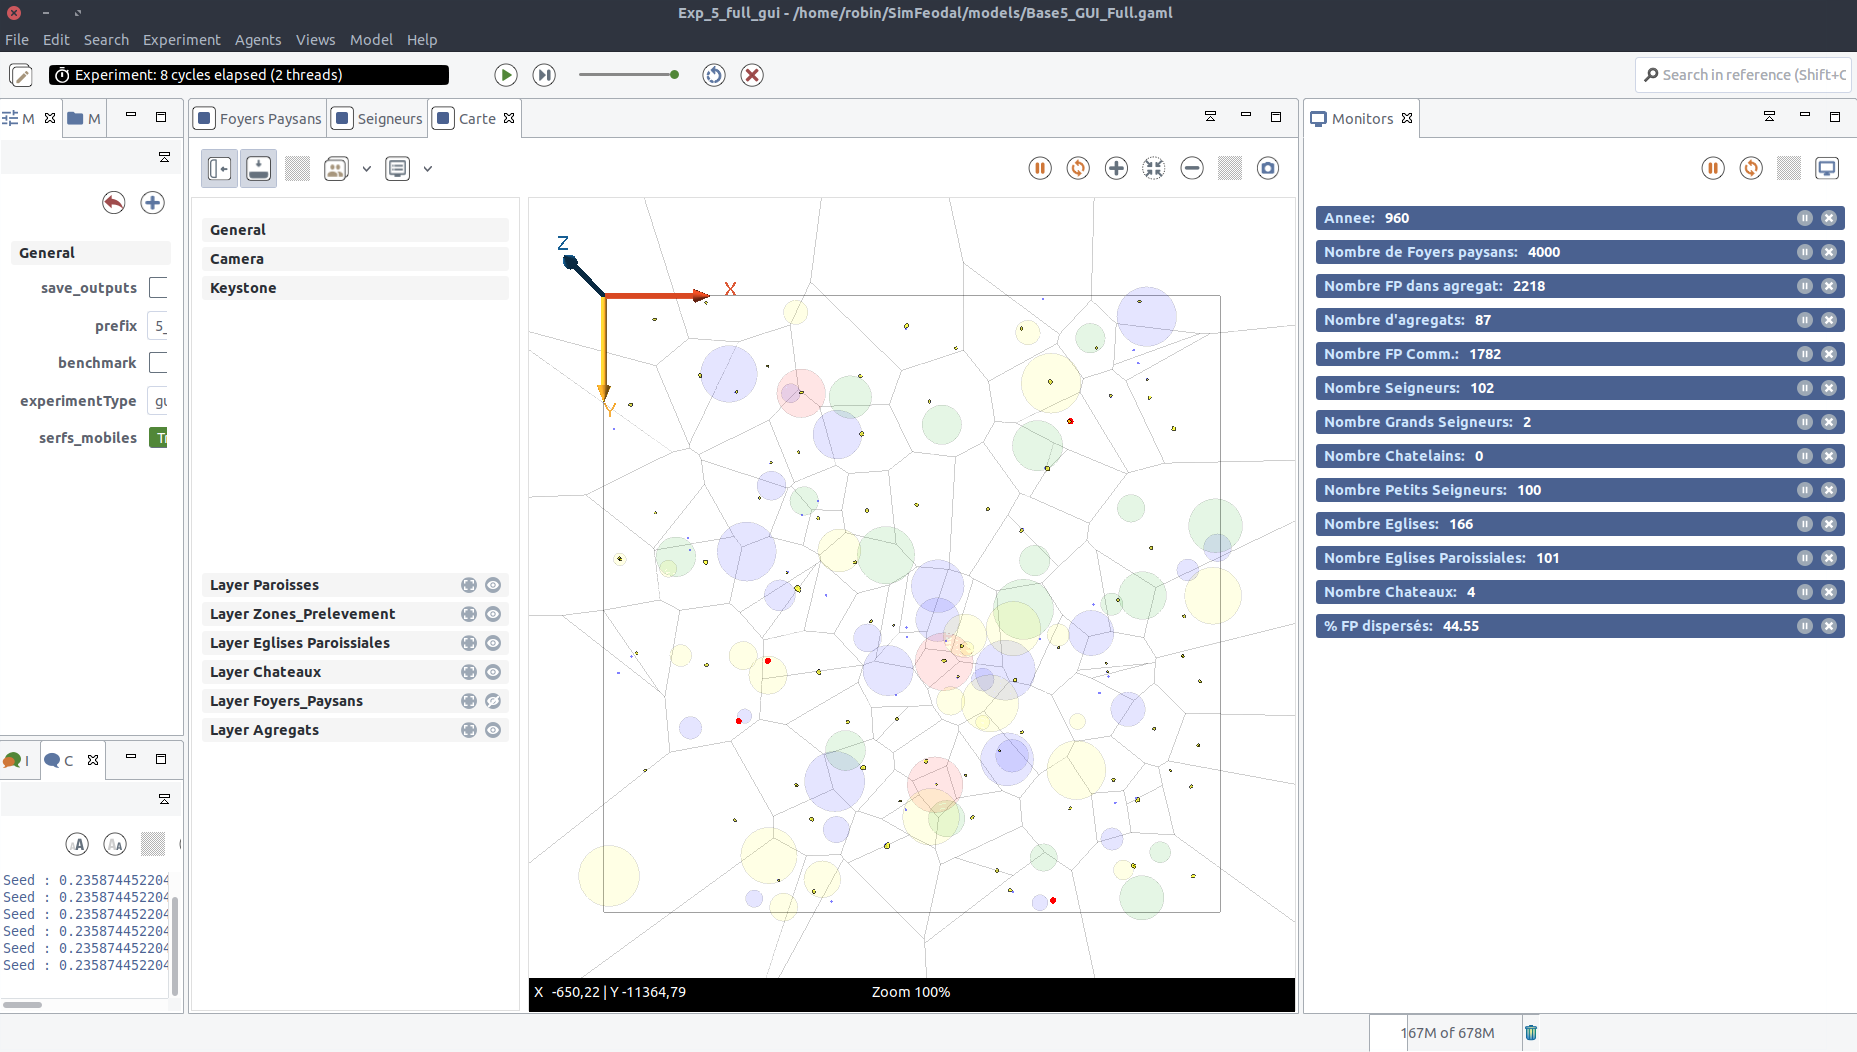
\includegraphics[width=\linewidth]{img/SimFeodal_GUI_carte.png}
	\caption{Visualisation intégrée à l'interface graphique interne de SimFeodal : cartographie synthétique de l'espace modélisé.}
	\label{fig:simfeodal_gui_carte}
\end{figure}

	Ces indicateurs intégrés à l'interface graphique interne de SimFeodal permettent de mener une étape préalable à l'évaluation du modèle.
	Cette étape vise à effectuer un premier filtrage des simulations avant d'exécuter les expériences en elles-mêmes.
	L'ajout de cette interface graphique vient donc renforcer l'outillage d'évaluation de SimFeodal.
	A cette étape, il manque encore un outil véritablement adapté à l'analyse conjointe des réplications du modèle, a posteriori de l'exécution des nombreuses réplications.

	\subsection{Générer les indicateurs}

	La production des indicateurs doit nécessairement être réalisée en aval de l'exécution des simulations (\og \textit{offline}\fg{} dans \cite{grignard_agent-based_2017}).
	Il faut pour cela disposer d'outils adaptés au traitement des données produites, c'est-à-dire répondant aux contraintes identifiées auparavant (\autoref{subsec:donnees-indicateurs}).
	La contrainte principale est d'être en mesure de gérer la masse de données produites.
	On l'a vu, cela élimine d'office les outils de type tableurs, ou encore les outils de manipulation graphique de données les plus courants.
	Pour les raisons évoquées dans le chapitre 1 (\hl{Positionnement : pourquoi utiliser des outils libres ?}), seules les solutions techniques libres étaient envisageables.

	Certains outils graphiques, basés sur des logiciels libres en arrière-plan (PSPP, R Commander, Orange), sont extrêmement aisés à prendre en main et auraient pu constituer un bon choix.
	Pourtant, avec une trentaine d'indicateurs à produire pour chaque expérience, donc de manière régulière, nous avons préféré nous tourner vers des outils plus orientés vers une interface en ligne de commande (\textit{Command Line Interface}, abrégés \textit{CLI}).

	L'utilisation de CLI a plusieurs intérêts gravitant autour de la reproductibilité des traitements.
	En premier lieu, ils permettent une adaptation aisée et rapide aux différents jeux de données.
	Ainsi, partant du principe que les données générées par les réplications et expérimentations sont de même structures, il suffit généralement de modifier le chemin d'entrée des fichiers résultants pour reproduire à l'identique une analyse sur un nouveau jeu de données.

	De manière plus technique, on peut remarquer que les différents indicateurs de sortie de simulation choisis présentent souvent des caractéristiques communes, aussi bien dans le traitement nécessaire que dans les formats (graphiques) produits.

	Par exemple, la grande majorité des indicateurs reposent sur une première agrégation des données par réplication et pas de temps simulé, puis par une seconde agrégation montrant la variabilité des situations générées, au niveau de l'expérimentation\footnote{
	On peut considérer ces agrégations comme une succession d'opération imbriquées : pour montrer l'évolution d'un indicateur tel que le taux de foyers paysans dispersés au cours du temps simulé, il faut (1) calculer le ratio entre nombre de foyers paysans dispersés et nombre total de foyers paysans, (2) pour chacun des pas de temps simulé, (3) pour chaque simulation, (4) pour l'ensemble des réplications d'une expérience, (5) éventuellement pour chacune des expériences d'une phase plus large d'expérimentation qui ferait varier des valeurs de paramètres.
	}.
	En terme de manipulation de données, seuls le calcul de la variable à mobiliser, et éventuellement l'agent caractérisé -- la variabilité du nombre de foyers paysans et la variabilité du nombre d'agrégats ne diffèrent que par le type d'agent sur lequel le calcul est effectué --, sont ainsi à adapter dans ces nombreux indicateurs de sortie.
	Les variations, en terme de code-sources, sont donc le plus souvent des adaptations minimes (nom de l'agent, type d'agrégation\ldots).
	Le recours à des traitements en \textit{CLI} permet ainsi un simple copier/coller, voir la création de fonctions dédiées, pour effectuer ces traitements très récurrents.

	Au niveau des sorties graphiques, on peut aussi remarquer que la structure des graphiques, en elle-même, est assez largement identique : on représente les pas des temps (les années simulées) en abscisse, un indicateur statistique en ordonnée, et la variabilité sous la forme de \textit{box-plot} minimalistes (\og \textit{minimal boxplot}\fg{}, promus par Edward Tufte pour minimiser le ratio données-encre \autocite[123-125]{tufte_visual_2001}).
	En disposant d'un environnement de type \textit{CLI}, et qui plus est en faisant usage de solutions graphiques construites sur une syntaxe régulière et générique (voir \cnameref{par:visualisation-pipeline}, \cpageref{par:visualisation-pipeline}), il devient très confortable de générer les différents indicateurs de sortie souhaités, puisqu'il suffit d'adapter les graphiques déjà conçus.

	Avec ces solutions logicielles d'analyse de données et de visualisation, il est facile de concevoir et d'implémenter les codes informatiques nécessaires à la génération des indicateurs de sortie de simulation.
	De plus, l'exécution de ces programmes est extrêmement rapide :  les différents fichiers de sortie de simulation sont lus et parcourus une unique fois pour en tirer toutes les variables nécessaires à l'établissement des indicateurs.

	\paragraph*{}
	En ayant choisi de mener une évaluation \textit{a posteriori} -- plutôt qu'en direct -- basée sur l'observation d'indicateurs générés -- par des outils adaptés au traitement de données massives -- de manière automatisée, on dispose donc, pour chaque expérience, d'un ensemble de fichiers numériques : chacun des indicateurs  de sortie est contenu dans un fichier unique, dans un format facilement exploitable et ré-utilisable. 

	\subsection{Organiser les indicateurs en rapports paramétrables}

	Du point de vue de la manipulation, la création de fichiers informatiques indépendants correspondant aux différents indicateurs de sortie de simulation est extrêmement pratique : on peut facilement les identifier, les transférer et les adapter, par exemple pour en rendre le contenu plus compréhensible par un public différent.

	En revanche, du point de vue de la comparaison des résultats, cette forme n'est pas la plus adaptée.
	Si l'on peut facilement comparer un même indicateur portant sur deux expériences différentes, la tâche se complique quand il s'agit d'avoir une vision globale des différences dans les indicateurs entre deux expériences.
	Pour cela, la démultiplication des fichiers correspondant aux indicateurs se révèle rapidement être un obstacle : l'utilisateur est en effet amené à jongler entre de très nombreux fichiers.
	
	\paragraph{Les rapports comme instruments de comparaison}
	Pour faciliter la comparaison d'indicateurs multiples -- et d'une forte diversité --, il est nécessaire de les organiser au sein d'une structure englobante.
	Nous entendons ici par organisation, une présentation structurée, suivant un certain ordre, identique selon les expériences, adaptée à une évaluation des résultats.
	Pour cela, nous avons choisi d'organiser les indicateurs de sortie de simulation au sein de \og rapports \fg{}.
	Cela permet, même en présence de nombreuses expériences, de rassembler l'ensemble des indicateurs de sortie propres à chacune dans un unique fichier, à la structure toujours similaire.
	Un premier apport, majeur, concerne l'archivage des sorties de simulation.
	Avec des rapports comprenant l'ensemble des indicateurs de sortie de chaque expérience d'un modèle, il est ainsi simple de conserver des traces de l'ensemble des versions et sous-version d'un modèle.
	Cela permet de garantir une certaine pérennité à ce modèle, à sa documentation, et ainsi simplifie le travail rétrospectif de caractérisation de l'évolution d'un modèle.	
	
	L'intérêt majeur de la structuration en rapports est surtout de faciliter la comparaison des expériences, c'est-à-dire des indicateurs de sortie des différentes expériences.
	On peut ainsi, par exemple, placer côte à côte, visuellement, deux rapports rendant compte de deux expériences différentes, et, en les faisant défiler simultanément, comparer point par point, c'est-à-dire indicateur par indicateur, leurs résultats respectifs, de manière visuelle et intuitive.

	Les formes que peuvent prendre des rapports, tout autant que les modalités de leur production, sont multiples et extrêmement diverses.
	La forme la plus simple et courante consiste à produire manuellement le rapport en insérant les indicateurs adaptés au fur et à mesure, par exemple dans un traitement de texte.
	A l'opposé, on peut noter les possibilités de créations entièrement automatisées de rapports complets, comprenant par exemple des descriptions et commentaires textuels générés à la volée, en fonction d'expressions conditionnelles\footnote{Voir par exemple l'application \og SOFIE\fg{} de l'Observatoire des Territoires du Commissariat général à l'égalité des territoires (CGET), qui génère automatiquement des commentaires relatifs aux inégalités femmes/hommes dans l'accès à l'emploi. Les commentaires propres aux types d'inégalités majeures de chaque EPCI sont produits de manière automatique depuis les données. \href{http://outils.observatoire-des-territoires.gouv.fr/sofie/}{http://outils.observatoire-des-territoires.gouv.fr/sofie/}
	}.

	Pour SimFeodal, nous avons choisi de restreindre au maximum la manipulation manuelle.
	On souhaitait générer un rapport entièrement automatique, ne requérant pas d'action spécifique en dehors du choix des données depuis lesquelles créer les indicateurs.
	A l'inverse, on a choisi de ne pas ajouter de fonctionnalité de commentaire automatique des indicateurs de sortie : la richesse -- et la difficulté-- d'une approche interdisciplinaire telle que la notre est constituée par la multiplication des analyses et points de vue.
	Il n'y avait donc aucun besoin de générer des commentaires standardisés et automatiques, forcément moins aboutis que les commentaires de chacun des co-concepteurs du modèle.
	Le rapport produit (\cref{fig:simfeodal_rapport_mini}) n'intègre donc que les indicateurs, sous forme de tableaux et de graphiques.
	Ces indicateurs sont organisés par partie, en l'occurrence en fonction du type d'entités et de comportement qu'ils décrivent.

	\begin{figure}[H]
		\captionsetup{width=\linewidth}
		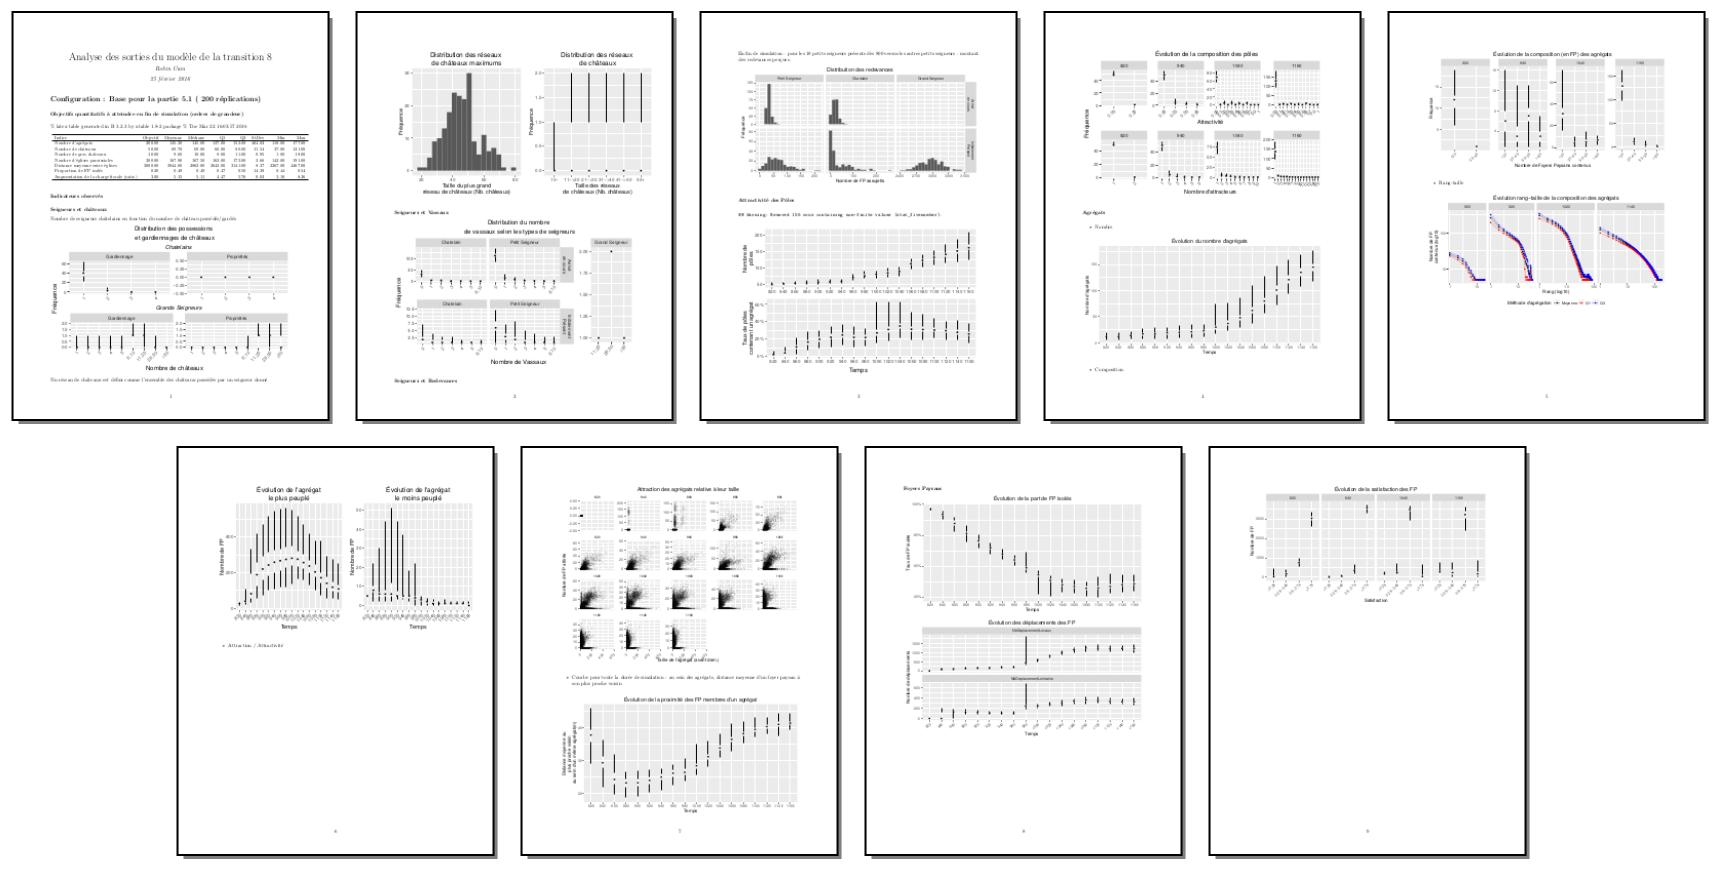
\includegraphics[width=\linewidth]{img/SimFeodal_Rapport_exemple.png}
		\caption{Un exemple de rapport automatique généré pour une expérimentation (étape 0) de SimFeodal. La version en taille réelle est reproduite en \hl{annexe X}.}
		\label{fig:simfeodal_rapport_mini}
	\end{figure}

\clearpage
	\paragraph{Structurer des rapports pour aller vers la reproductibilité des analyses}
	On a donc fait le choix de se baser sur des rapports automatisés et minimalistes, ne contenant que les indicateurs dans une forme structurée.
	Ce choix s'appuie sur des raisons multiples, qui ont toutes en commun une recherche de reproductibilité des résultats et des analyses menées.
	Une reproductibilité théorique (\hl{encore une ref au positionnement}), puisque les résultats de simulation doivent pouvoir être analysés et reproduits par des chercheurs potentiellement intéressés.
	Mais cette recherche de reproductibilité est aussi pratique, rendue aussi nécessaire par les méthodes de modélisation suivies.
	Tel qu'explicité auparavant (\cref{subsec:capter-replications,subsec:capter-experiences}), celles-ci s'appuient sur de nombreux allers-retours, ce qui requiert une capacité constante à reproduire et à affiner des résultats déjà observés.
	
	La quantité d'expériences requises pour arriver à un état satisfaisant du modèle est tributaire de ces allers-retours, et le nombre de rapports qu'il faut pouvoir produire est important.
	La fréquence de production de ces rapports est forte, et le modélisateur a alors tout intérêt à en fluidifier et accélérer le processus de création.
	
	Dans une telle situation, la création d'un rapport automatisé garantit une calcul et une production simplifié et rapide des indicateurs sur les nouvelles données.
	Cela permet un examen des sorties de simulation presque immédiatement après leur exécution.
	Cette automatisation permet aussi de mener une seconde évaluation -- après le pré-filtrage constitué par l'observation d'indicateurs en direct -- du bon déroulement \og interne \fg{}\footnote{
		Au sens de l'évaluation interne, c'est-à-dire du bon fonctionnement, exempt de \textit{bugs}, du modèle de simulation implémenté.
	}.
	Le caractère fixe d'un rapport automatisé se base ainsi sur une structure de données contraignante, par exemple constitués en \textit{n} fichiers dotés de plusieurs colonnes spécifiquement attendues.
	Les caractéristiques de ces données sont elles-mêmes contraignantes.
	Un rapport automatisé ne fonctionne, par exemple, qu'en présence d'un nombre pré-défini de réplications complètes.
	En l'absence d'un de ces critères dans des données en sortie de simulation, le rapport ne peut être généré et émet une erreur.
	Par exemple, si le nombre de réplications est plus faible qu'attendu, ou encore si tel attribut d'un agent a changé de type informatique, la création du rapport échoue.
	La présence ou non de cette erreur constitue donc un nouveau filtre de vérification de la validité du modèle.
	Cela permet, là encore, de détecter des simulations qui présenteraient des comportements incomplets ou aberrants en terme de production de données.

	Un autre intérêt majeur des rapports, déjà pointé en avantage des outils de type \textit{CLI} est leur adaptabilité.
	On a vu (\hl{chap. 3}) que les indicateurs à examiner sont nombreux et surtout, évolutifs, dans le sens où ces indicateurs ont fortement été modifiés, remplacés, affinés, au cours des étapes de paramétrage de SimFeodal.
	L'utilisation de rapports automatiques permet de minimiser le nombre de modifications à effectuer en cas de changements d'indicateurs.
	Le programme informatique qui génère les rapports s'appuie ainsi sur un code-source unique, générique aux simulations de chaque modèle.
	Lors d'un changement d'indicateurs, il suffit alors de modifier ce code-source en une seule place, et tous les appels à ce programme seront alors modifiés en conséquence.
	À partir de là, pour mettre à jour l'ensemble des rapports déjà produits, c'est-à-dire regroupant les indicateurs de chacune des expériences passées, il suffit de ré-exécuter la routine de production des rapports.
	
	Dans le cas de SimFeodal, caractérisé par de fréquents changements dans la forme et le calcul des indicateurs, cela a représenté un gain de temps et d'efficacité très conséquent.
	Par exemple, lors de certaines phases de paramétrage, on pouvait être amenés à faire évoluer le modèle quotidiennement et à tester, à cette même fréquence, plusieurs jeux de paramètres.
	Il fallait donc analyser les résultats de plusieurs expériences chaque jour, et régulièrement ajouter des indicateurs graphiques afin d'affiner l'évaluation.
	Ces indicateurs devaient aussi être ajoutés aux expériences des jours précédents, et au final, on re-générait parfois jusqu'à une plus d'une dizaine de rapports sur des cycles temporels courts de quelques jours.
		
	Par extension, cette même démarche d'automatisation, basée sur l'utilisation d'outils de type \textit{CLI}, devrait pouvoir s'appliquer à l'identique, avec les mêmes avantages, dans le cadre plus large de l'évaluation visuelle de modèles (\hl{ref chap 3, section 3.1.4}).

%	\begin{encadre}{Générer les rapports avec \texttt{R} et \texttt{knitr}}{technique-rapports-knitr}
%
%		\hl{Encadré sur les rapports automatiques, le \textit{\og litterate programming}\fg, le choix et le paramétrage de knitr + lien vers le code-source des rapports.}
%
%	\end{encadre}


	\paragraph{Dépasser les limites de la compatibilité d'ensemble}
	En réalité, la démarche de reproductibilité des rapports constitue plus un objectif théorique qu'un stade, \og reproductible\fg{} qu'il serait possible d'atteindre.
	Il s'agit ainsi plus de s'inscrire dans la voie de la reproductibilité que de chercher à parvenir à cet objectif largement inaccessible dans les faits.
	
	Comme explicité dans l'hl{encadré 3.2} sur l'incrémentalité des indicateurs, une limite forte empêche d'atteindre une reproductibilité absolue des analyses du comportement des différentes versions de SimFeodal.
	Les données générées par les différentes versions du modèle ne sont en effet pas systématiquement \og compatibles \fg{}.
	On entend par là qu'elles ne présentent pas toute exactement la même structure, à commencer par les variables enregistrées.
	Quand bien même il aurait été choisi dès le départ d'enregistrer le plus de sorties possibles, la reproductibilité de l'analyse échoue sur les données produites par le modèle et ses nombreuses versions : le modèle évolue, et avec lui, certaines variables apparaissent et d'autres deviennent caduques.
	La structure contraignante et précise des données nécessaires à la génération des rapports ne peut être entièrement satisfaite.
	La prise en compte de l'évolution du modèle demande une adaptation régulière -- mais aussi rare que possible -- des programmes qui génèrent ces rapports.
	
	On ne peut donc satisfaire globalement à un objectif de reproductibilité, mais il est toutefois possible de limiter la déviance à cette ambition.
	Pour cela, on peut agencer les différentes versions du modèles au sein de \og générations\fg{} de modèle, c'est-à-dire d'ensembles de versions présentant des attributs comparables et générant des données de même structure.
	Plutôt que d'adapter le code-source des rapports à chaque nouvelle version du modèle, ou encore de ne jamais l'adapter et donc d'être tributaire de la structure des toutes premières versions du modèle, cela constitue un choix intermédiaire qui permet de limiter le nombre de variantes de rapports.
	Cette approche suit les grandes lignes du développement logiciel général. Les itérations successives d'un logiciel sont constituées de versions \og majeures\fg{} -- les générations de modèles dans notre cas --, qui n'assurent pas nécessairement de compatibilité avec les versions majeures précédentes, et de versions \og mineures\fg{}, dans lesquelles la compatibilité est assurée\footnote{
		Par exemple, un fichier de dessin vectoriel créé avec le logiciel Adobe Illustrator 15.0 ne sera pas lu correctement avec une version 14.0.
		Ce fichier présentera toutefois un compatibilité parfaite avec les versions 15.1 à 15.\textit{n} du logiciel.
	}.
	
	Pour revenir aux rapports voués à l'évaluation d'un modèle, en inscrivant les différentes versions du modèle -- et des programmes générant les rapport correspondant -- dans des sous-ensemble de versions, les \og générations\fg{}, les différents rapports peuvent être considérés comme reproductibles et automatiques au sein de ces générations.
	Pour SimFeodal, cela implique d'organiser les différentes versions du modèle -- résultant des étapes de paramétrage, \hl{cf. chap4} -- au sein de grandes générations, à chaque changements structurels des mécanismes ou données produites par le modèle.
	
	\hl{Ajouter un schéma avec les générations, versions et sous-versions}
	
	\paragraph{Les rapports, des instruments suffisants ?}
	
	A l'issue de la conception et de l'implémentation de ces rapports automatiques, on dispose donc, pour chaque expérience, d'un document aisément partageable et lisible.
	Ces documents s'enrichissent, au fur et à mesure des générations de modèles, de nouveaux indicateurs, et sont comparables au sein de ces générations.
	Cela pourrait constituer la dernière étape de la création d'outils d'évaluation d'un modèle, dans la limite d'un nombre de versions ou de génération de modèles assez restreint.
	
	SimFeodal, comme c'est souvent le cas dans les modèles à base d'agent, a toutefois été caractérisé par une forte quantité d'allers-retours entre le modèle et ses résultats, entraînant à chaque fois de nouvelles expérimentations (cf. \cref{sec:sorties-simfeodal}). 
	
	On a vu que la manipulation d'un grand nombre d'indicateurs, même pour une quantité restreinte d'expériences, disqualifiait l'usage de fichiers individuels et poussait à l'usage de rapports structurés.
	Avec un grand nombre d'expériences, les mêmes limites apparaissent pour les rapports : la masse d'expériences rend partiellement caduque l'utilisation unique des rapports automatiques.
	Il est en effet aisé de comparer, sur un même écran d'ordinateur, deux ou trois rapports, mais dès lors qu'il faut en comparer un plus grand nombre, la manipulation conjointe des rapports devient complexe, tout autant que d'avoir une vision globale des résultats principaux de chaque expérience.

\clearpage
	\subsection{Organiser les rapports : Dashboards}\label{subsec:dashboards}

	Pour être en mesure de comparer de nombreux éléments, il est nécessaire de passer d'une exploration linéaire, fondée sur le visualisation successive de chacun des indicateurs, à une exploration globale et interactive.
	En pratique, plutôt que de faire défiler visuellement les nombreuses pages d'indicateurs, mieux vaut une interface présentant les points clefs de l'évaluation et qui permette d'entrer dans le détail de chacun des indicateurs dans un second temps, sur demande.
	Comme le résume le \og mantra\fg{} de l'analyse visuelle (\og \textit{Visual information-seeking mantra}\fg{}) de \citeauteur{shneiderman1996eyes} :
\begin{quote}
	\centering
	\noindent\og Overview first, zoom and filter, then details on demand\fg{}\\
	\mbox{}~ \hfill \cite[\ppno~2]{shneiderman1996eyes}
\end{quote}
	

	\subsubsection{Les \textit{dashboards}}

	Cette logique, assez universelle désormais, est celle qui préside à la création des nombreux \og tableaux de bord \fg{}, ou \og \textit{dashboards} \fg{} que l'ont voit émerger depuis la fin des années 1990.
	Rob Kitchin et ses co-auteurs définissent ainsi les \textit{dashboards}, en s'appuyant sur les travaux de Few notamment :

	\begin{quotation}
		\og For Few [\autocite[p.34]{few_information_2006}] a ‘dashboard is
		a visual display of the most important information needed to achieve one or more objectives; consolidated and arranged on a single screen so the information can be monitored at a glance’.
		Just as a car dashboard provides critical information needed to operate the vehicle at a glance, indicator dashboards provide key information for running companies or cities (\st{Dubriwny \& Rivard, 2004})[\autocite{rivard_are_2004}].\fg{}\\
		\mbox{}~ \hfill \cite[p. 11]{kitchin_knowing_2015}
	\end{quotation}

	Très répandus dans le monde de l'informatique décisionnelle (\textit{Business Intelligence, BI}), ces outils permettent d'explorer des données d'entreprises, par exemple des résultats financiers.
	Pour ce faire, ils mettent en avant, dans une interface unique, des indicateurs clés (\textit{Key Performance Indicators, KPI}), qu'il est ensuite possible de filtrer et d'affiner, par exemple par sélection de différents intervalles temporels.

	Les \textit{KPI} jouent le rôle d'indicateurs synthétiques, c'est-à-dire qu'ils s'adressent à des gestionnaires, par exemple des \textit{managers}, qui ont une expertise importante sur les résultats produits.
	Les utilisateurs des \textit{dashboards} ne sont donc pas des analystes, à même d'explorer eux-mêmes les données mobilisées, mais plutôt des thématiciens qui se fondent sur les indicateurs présentés pour prendre des décisions.

	La dichotomie \og analyste/décisionnaire\fg{} s'exprime aussi dans le domaine de la recherche, et notamment dans la recherche en géographie urbaine à visée applicative.
	Avec l'avènement des données massives et de leur prise en compte pour la gestion des villes (\textit{smart cities}), les géographes se sont aussi penchés sur des outils de ce type.
	En résulte une utilisation de plus en plus fréquente de \textit{dashboards} en géographie urbaine (\og \textit{city-dashboards}\fg{}, \cite{roumpani_creating_2013, kitchin_knowing_2015, batty_perspective_2015}).

	Le parallèle avec le monde de l'informatique décisionnelle est en effet présent dans les types d'utilisateurs et de producteurs de ces outils.
	Il s'agit de mettre à disposition d'experts thématiques (les décideurs publiques) des indicateurs clés, issus de calculs parfois complexes.
	Cela afin de leur permettre d'évaluer une situation donnée et de prendre les décisions politiques adéquates.

	Le constat ayant mené à l'apparition des premiers \textit{dashboards}, tant en informatique décisionnelle qu'en géographie urbaine, est identique.
	Les informations nécessaires à l'évaluation d'une situation (financière, relative aux politiques publiques\ldots) sont de plus en plus nombreuses et hétérogènes.
	Les indicateurs permettant de mener ces évaluations, pensés pour les décideurs qui en feront usage (\textit{managers}, acteurs publiques\ldots), se démultiplient et se diversifient aussi par conséquence.

	Inspiré autant par l'usage \textit{BI} que par l'usage géographique, nous considérons que ces outils peuvent se révéler utiles dans l'évaluation de modèles de simulations complexes.
	Les enjeux sont en effet les mêmes : permettre à des thématiciens de comprendre et d'évaluer les sorties d'un modèle, à l'aide d'indicateurs nombreux et complexes présentés de manière transparente relativement à cette complexité.

	Ce positionnement méthodologique s'inscrit pleinement dans la démarche de co-construction interdisciplinaire de SimFeodal.
	On y retrouve ainsi la même logique qui anime les dashboards : une évaluation menée par des thématiciens qui s'appuient pour cela sur des indicateurs clefs (\hl{ref. aux indicateurs les plus importants dans le chap 3}) et précisent leur analyse à l'aide d'indicateurs secondaires présentés sous forme d'un panel varié de visualisations.
	Nous avons donc choisi de ré-organiser les rapports initialement produits pour leur donner une forme plus adaptée à ces enjeux, sous forme de \textit{dashboards}.

	\subsubsection{SimVADB}\label{subsubsec:simvadb}

	Les \textit{dashboards} font souvent usages de représentations graphiques très métaphoriques des tableaux de bords automobiles.
	On y retrouve fréquemment une forte mise en valeur d'indicateurs numériques simples au travers de représentations \og skeuomorphes\fg{}, c'est-à-dire qui reprennent l'apparence physique des objets symbolisés.
	On retrouve communément, par exemple, des indicateurs représentés sous forme de jauges (\textit{gauge charts}), de thermomètres (\textit{thermometer charts}), ou encore de voyants d'alerte et autres témoins lumineux (\cref{fig:skeuomorphism})).
	
	\begin{figure}[H]
		\centering
		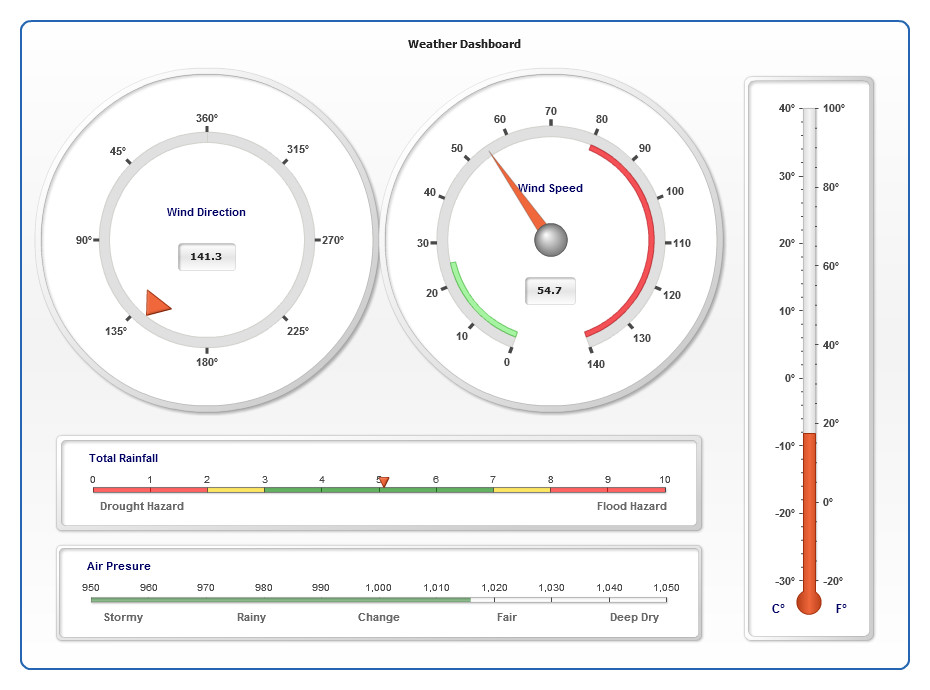
\includegraphics[width=.8\linewidth]{img/skeuomorphism.jpg}
		\caption{Un exemple de représentations visuelles courantes dans les \textit{dashboards}. Tiré de \textcite{pandre_charts_2011}}
		\label{fig:skeuomorphism}
	\end{figure}
	
	
	Pour SimFeodal, les indicateurs étant assez fortement conçus et structurés (\hl{chap. 3}), nous n'avons pas ressenti le besoin de faire appel à ce type de représentation.
	Nous avons donc emprunté aux \textit{dashboards} la logique d'organisation visuelle des indicateurs plutôt que les modes de visualisation en eux-mêmes.
	Pour faciliter la transition pour l'utilisateur, on cherchait ainsi à produire un \textit{dashboard} au plus proche, visuellement, des rapports automatiques qui les précédaient.

	On a pour cela développé un \textit{dashboard} adapté à SimFeodal, nommé SimVADB\footnote{
	\textbf{S}imulation \textbf{V}isual \textbf{A}nalysis \textbf{D}ash\textbf{B}oard.\\
	Cette application a rapidement été remplacée par l'itération suivante (SimEDB, voir \cref{subsec:explo-interactive}), et n'a donc dans les faits jamais été complètement finalisée. On en trouve une trace, fonctionnelle mais incomplète (les versions ultérieures n'ont pas été enregistrées dans l'outil de versionnement), dans ce dépôt logiciel :
	\href{https://github.com/RCura/SimEDB/tree/2cd22c7ccfbcf31f4a09550c2396932c46ef2622}{https://github.com/RCura/SimEDB/tree/2cd22c7c}
	}.
	Dans un premier temps, on souhaitait simplement ré-organiser le code-source produisant les rapports automatiques, afin de convertir ces rapports en \textit{dashboards}.
	Cela a été effectué au moyen d'outils permettant de générer des applications en ligne, sans changer de langage de programmation.
	Dans ce cas, on s'est appuyé sur la librairie logicielle \textsf{Flexdashboard} \autocite{iannone_flexdashboard_2018}.
	
	Le passage du rapport automatique au \textit{dashboard} illustre l'un des grands intérêts des outils de type \textit{CLI} : dans le cas de SimVADB, il a suffit de ré-organiser le code, sans modifier à aucun moment les fonctions de calcul et de création des indicateurs de sortie de simulation.
	Les codes \ref{lst:code-rapport} et \ref{lst:code-dashboard} illustrent la facilité de cette modification.
	Il s'agit véritablement de placer les différentes fonctions dans des blocs graphiques.
	Ces modifications minimes augmentent toutefois considérablement la convivialité et la facilité de l'analyse de résultats de sortie d'un modèle.
\clearpage

\lstset{frame=shadowbox, tabsize=2}
\noindent\begin{minipage}[t]{.44\textwidth}
{\footnotesize
	\begin{lstlisting}[caption={Pseudo-code du rapport automatique.},frame=tlrb, captionpos=b, label = {lst:code-rapport}]
# Agent de type A
	afficher('Agent de type A')
	
	print('Indicateur 1')
	calcul_indicateur_1 {...}
	affichage_indicateur_1 {...}
	
	afficher('Indicateur 2')
	calcul_indicateur_2 {...}
	affichage_indicateur_2 {...}
# Agent de type B
	afficher('Agent de type B')
	[...]
	\end{lstlisting}
}
\end{minipage}\hfill
\begin{minipage}[t]{.53\textwidth}
{\footnotesize
	\begin{lstlisting}[caption={Pseudo-code du dashboard.},frame=tlrb, captionpos=b, label = {lst:code-dashboard}]
onglet{titre = 'Agent de type A',
	sous_onglet{titre = 'Indicateur 1',
		calcul_indicateur_1 {...}
		affichage_indicateur_1 {...}
	},
	sous_onglet{titre = 'Indicateur 2',
		calcul_indicateur_2 {...}
		affichage_indicateur_2 {...}
	}
},
onglet{titre = 'Agent de type B',
	[...]
}
	\end{lstlisting}
}
\end{minipage}
	
	Comme dans l'exemple de code, on a préféré organiser les indicateurs au seins d'onglets plutôt que de les présenter dans des pages successives.
	Les onglets de premier niveau représentaient les types d'agent, et des onglets de second niveau permettaient de visualiser l'ensemble des indicateurs associés à ces agents (\cref{fig:mockup_simvadb}).

\begin{figure}[H]
	\centering
	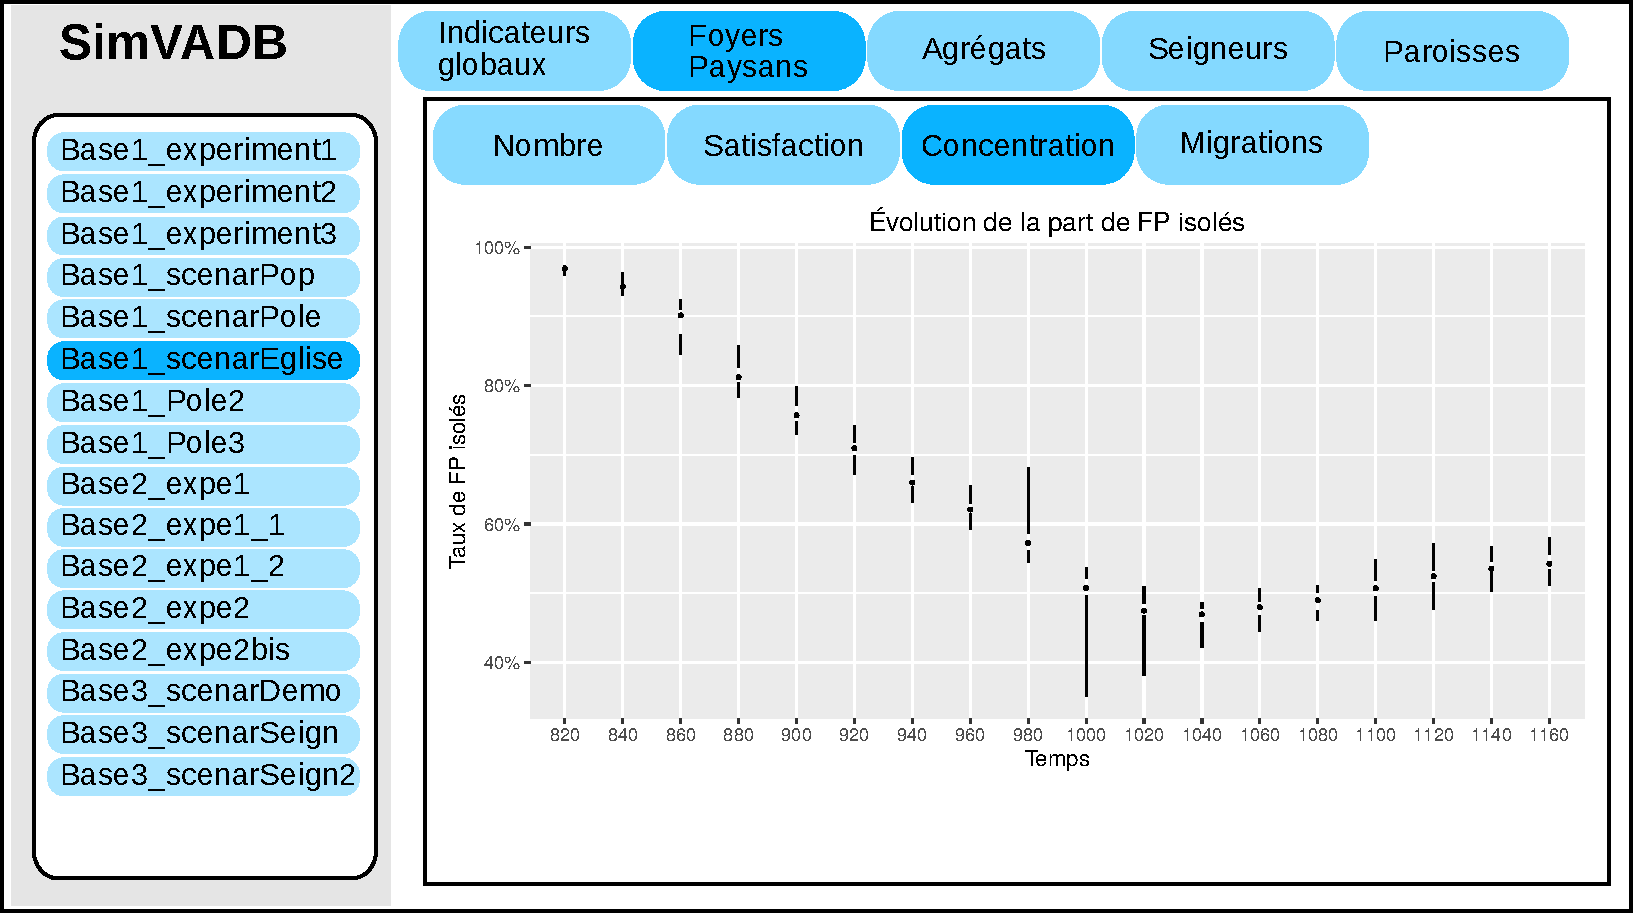
\includegraphics[width=\linewidth]{img/simvadb_mockup.pdf}
	\caption{Un \textit{mock-up} de la première interface de SimVADB, un \textit{dashboard} dédié à la visualisation des indicateurs de sorties de simulation de SimFeodal.}
	\label{fig:mockup_simvadb}
\end{figure}

	Au niveau de l'interface utilisateur, SimVADB permettait de choisir, via un menu de sélection (partie de gauche dans la \cref{fig:mockup_simvadb}), les expériences passées dont on voulait visualiser les indicateurs de sortie (les deux niveaux d'onglets de la partie de droite).

	
	\paragraph{Les limites du \textit{dashboard}}
	Avec la multiplication des valeurs de paramètres testées, il est devenu plus efficace de regrouper les expériences au sein d'expérimentations.
	Celles-ci voient varier plusieurs paramètres, potentiellement avec de multiples valeurs de paramètres pour chacun.
	Elles constituent donc un ensemble d'expériences qui partagent des mécanismes et un jeu de paramètre par défaut communs.

	Avec le mode de sélection choisi dans SimVADB, basé sur le nom des expériences, il devenait plus difficile de sélectionner rapidement des ensembles d'expériences membres d'une même phase d'expérimentation.
	En effet, et comme illustré dans la \cref{fig:mockup_simvadb}, les noms d'expériences tendent à s'allonger, et avec leur masse augmentant, il est peu commode d'avoir à parcourir tout un long menu de sélection pour trouver les expériences souhaitées.
	De plus, malgré des tentatives de nommage régulières et explicites, la multiplication des expériences et expérimentations implique aussi une certaine confusion dans les types de mécanismes et valeurs de paramètres associés.
	Sans table de correspondance complète entre les noms des expériences et leurs valeurs de paramètres, il devenait impraticable de retrouver les différentes expériences mettant en avant, par exemple, des attractivités fortes par les pôles, une plus forte hiérarchisation des attracteurs ou encore des migrations lointaines facilitées.
	Le choix méthodologique d'interaction avec la plate-forme d'affichage des indicateurs, basé sur une sélection des expériences depuis leur nom, s'est donc révélé inadapté à la sélection et à l'exploration des sorties de SimFeodal.
	
	
	Au delà du soucis du mode d'interaction, qui aurait pu être amélioré, un autre problème apparaissait.
	Pour évaluer visuellement différentes configurations du modèle, on ne pouvait se contenter d'un simple affichage des données, au sein d'un outil de type présentoir interactif tel que SimVADB.
	Comme dit dans \hl{le chapitre 4}, le paramétrage de SimFeodal a ainsi reposé sur de nombreuses étapes d'évaluation des différentes version du modèle.
	L'approche d'analyse principale était donc la comparaison, point par point, entre les résultats des indicateurs de sortie de simulation des versions successives de SimFeodal.
	Un outil de présentation dynamique de résultats de sorties de simulations est certes plus adapté qu'un rapport statique, mais il ne constitue pas pour autant un outil adapté à la comparaison.
	S'il suffit pour de la restitution, par exemple dans le cadre du rapport systématique des résultats de SimFeodal, on ne peut s'appuyer uniquement sur une succession d'évaluations visuelles pour appréhender l'étendue des changements apportées par une modification des valeurs de paramètres.

	\subsection{Interagir avec les rapports : exploration interactive}\label{subsec:explo-interactive}

	Face à la démultiplication des expérimentations, consécutive aux nombreuses étapes de paramétrage de SimFeodal (\hl{cf. chap 4}), il a fallu repenser la plate-forme d'évaluation des résultats.
	Pour cela, considérant que les simulations ne pouvaient être aisément appréhendées et sélectionnées par leur nom, numéro d'étape ou de version, il a été décidé d'adopter une posture plus proche de l'exploration du modèle en elle-même.
	C'est-à-dire de ne pas caractériser les simulations par un identifiant quelconque, mais plutôt par leur spécificité intrinsèque, c'est-à-dire la combinaison de valeurs de paramètres qui les rendent uniques.
	Ce faisant, au sein de la plate-forme d'exploration SimVADB, l'enjeu devenait plutôt la compréhension des effets des valeurs de paramètres sur les indicateurs que l'évaluation d'une simulation en particulier.
	Il fallait passer du descriptif, quelle qu'en soit la méthode, à du comparatif.
	
	Du point de vue de l'interface utilisateur, cela implique que la sélection ne se fasse plus par un unique critère (le nom de la simulation), mais au contraire sur du multi-critère.
	Par une succession de sélections, chaque paramètre pouvait constituer un nouveau filtre dans lequel on avait à choisir les valeurs à interroger (voir la \cref{fig:schema_parcoords} \textbf{(E)} de l'\cref{enc:parcoords}).

	La quantité de paramètres en entrée était importante et pouvait dès lors donner lieu à un mode de sélection complexe et fastidieux -- définir une par une les valeurs voulues pour chacun des 45 paramètres --.
	Nous avons choisi encore une fois de nous appuyer sur l'aspect visuel afin de permettre aux utilisateurs de SimVADB de choisir la ou les expérimentations à analyser.
	
	
	\paragraph{Visualiser avec des coordonnées parallèles }

	Pour cela, on a choisi de représenter les combinaisons de paramètres dans un graphique en \og coordonnées parallèles \fg{} (\textit{parallel coordinates}, d'après \cite{inselberg_parallel_1987}, voir \cite{few_multivariate_2006} par exemple pour une description plus succincte, illustrée et pratique).
	Ce type de graphique est en effet extrêmement pertinent pour représenter une information multi-dimensionnelle en ce qu'il permet de détecter graphiquement des \textit{clusters} d'individus statistiques\footnote{
		Ici, chaque expérience est un individu statistique.
		Il est caractérisé par un ensemble de variables, les différents paramètres, et les modalités de ces variables que cet individu emprunte (les valeurs de paramètres).
		Quand le nombre d'individus est important, les différentes \og courbes\fg{}, qui correspondent au profil des individus sur le graphique en coordonnées parallèles, peuvent se superposer et montrer des tendances similaires.
		Avec ce type de représentation, il est facile de visualiser les grandes classes d'individus constituées par ces \og tendances\fg{}, et donc de constater des distinctions entre les individus (les expériences) de manière visuelle.
	} \autocite[2]{heinrich_state_2013}, c'est-à-dire de faire ressortir visuellement les expériences dont les valeurs de paramètre sont proches.
	Notons bien que l'on parle ici des valeurs de paramètres, c'est-à-dire des conditions des expériences, et non des indicateurs de sortie.
	L'approche va ainsi des paramètres aux résultats : depuis des valeurs de paramètres choisies, on analyse la diversité des résultats.
%	L'approche inverse, souvent menée en simulation agent (\hl{ref à chap 3, exploration automatique}}), pourrait mener une classification des résultats de sortie pour reporter cette classification sur les valeurs de paramètres.

	
	\paragraph{Interagir avec des coordonnées parallèles}
	De plus, en matière d'interaction, on utilise fréquemment les graphiques en coordonnées parallèles en vue de filtrage.
	Cette opération est le plus souvent menée par des actions de \textit{brushing} (\og brossage\fg{}), c'est-à-dire de sélection graphique d'une zone en dessinant son étendue à la souris (voir \cref{enc:parcoords}).
	Ce type de sélection se révèle en effet souvent plus efficace et intuitive qu'une sélection textuelle plus systématique :
	
	\begin{quotation}\vspace{-0.5cm}
		\og Filtering is an operation that removes signals from its input. A filter reduces the number of lines to be rendered. In this sense, dynamic querying [...] is a filter, if implemented with brushing [...], which reduces clutter by putting the filtered lines in focus using some highlighting mechanism. Combining simple brushes using logical operators [...] further allows the user to formulate rather complex queries that might even achieve faster and more accurate results using parallel coordinates than using a Structured Query Language (SQL) [...].\fg{}\\
		\mbox{}~ \hfill \cite[p. 13]{heinrich_state_2013}
	\end{quotation}
	
	\begin{encadre}{Construction et utilisation interactive d'un graphique en coordonnées parallèles}{parcoords}

	La \cref{fig:schema_parcoords} illustre les étapes successives de construction d'un graphique en coordonnées parallèles, depuis le tableau statistique (\textbf{A}) jusqu'au graphique final (\textbf{D}).
	
	Pour cela, on projette les valeurs des variables sur des axes représentant chacune des variables (\textbf{B}).
	En normalisant la taille de ces axes et en les plaçant en parallèle (\textbf{C}), on peut alors tracer les \og profils\fg{} des variables en reliant les positions de chacun des individus statistiques sur chacun des axes (\textbf{D}).
	
	La seconde partie de la figure représente le mode d'interaction par \textit{brushing} : on \og brosse\fg{} sur chaque axe une sélection de valeurs à conserver (\textbf{E}).
	La sélection graphique est convertie en intervalles numériques et formalisée sous une forme classique (\textbf{F}) qui permet de filtrer les données sous-jacentes.
	Au final, cette opération renvoie le seul individu statistique répondant aux deux sélections graphiques (\textbf{G}).
	
	\begin{figure}[H]
	\centering
	\captionsetup{width=\linewidth}
	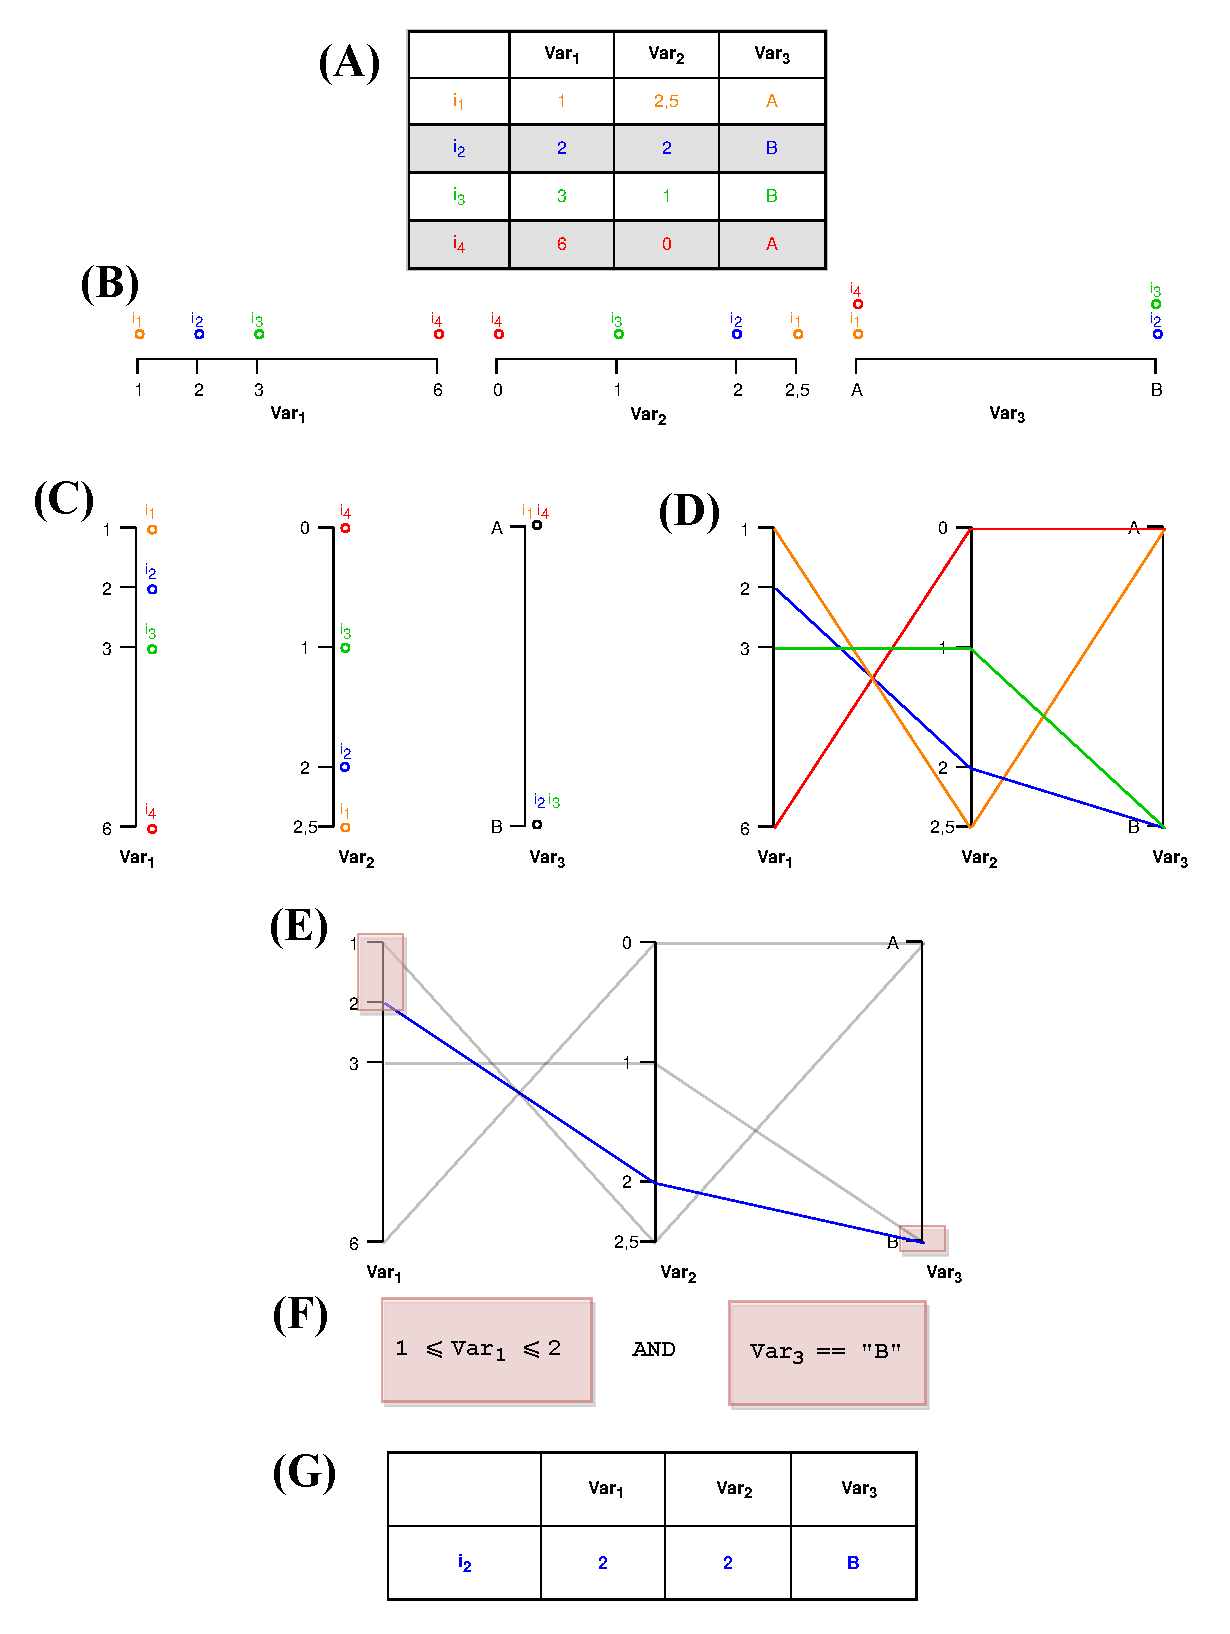
\includegraphics[width=.94\linewidth]{img/ParCoords_Brush.pdf}
	\caption{Construction d'un graphique en coordonnées parallèles et sélection interactive.\vspace{.1cm}}
	\label{fig:schema_parcoords}
	\end{figure}

	\end{encadre}


	Cette utilisation est aussi courante en géographie quantitative, et on la retrouve par exemple chez l'un des représentants de l'analyse spatiale des années 1990, Stewart Fotheringham.
	Cet auteur indique même l'usage du graphique en coordonnées parallèles en tant que filtre pour identifier des informations dans une autre dimension, spatiale ici : \og the data being displayed in parallel coordinates can be linked to a map and then brushed to highlight the locations of interesting lines displayed in \textit{m}-space on the parallel co-ordinates.\fg{} \autocite{fotheringham_trends_1999}.

	Appliqué aux données de SimFeodal, cette interface (\cref{fig:simvadb_dashboard}) se révèle particulièrement efficace pour sélectionner les configurations de paramètres à explorer.
	Ainsi, en \og brossant \fg{} quelques filtres manuellement (\cref{fig:simvadb_dashboard} - \textbf{A}), on arrive rapidement à isoler une expérience spécifique.

	\begin{figure}[H]
		\captionsetup{width=\linewidth}
		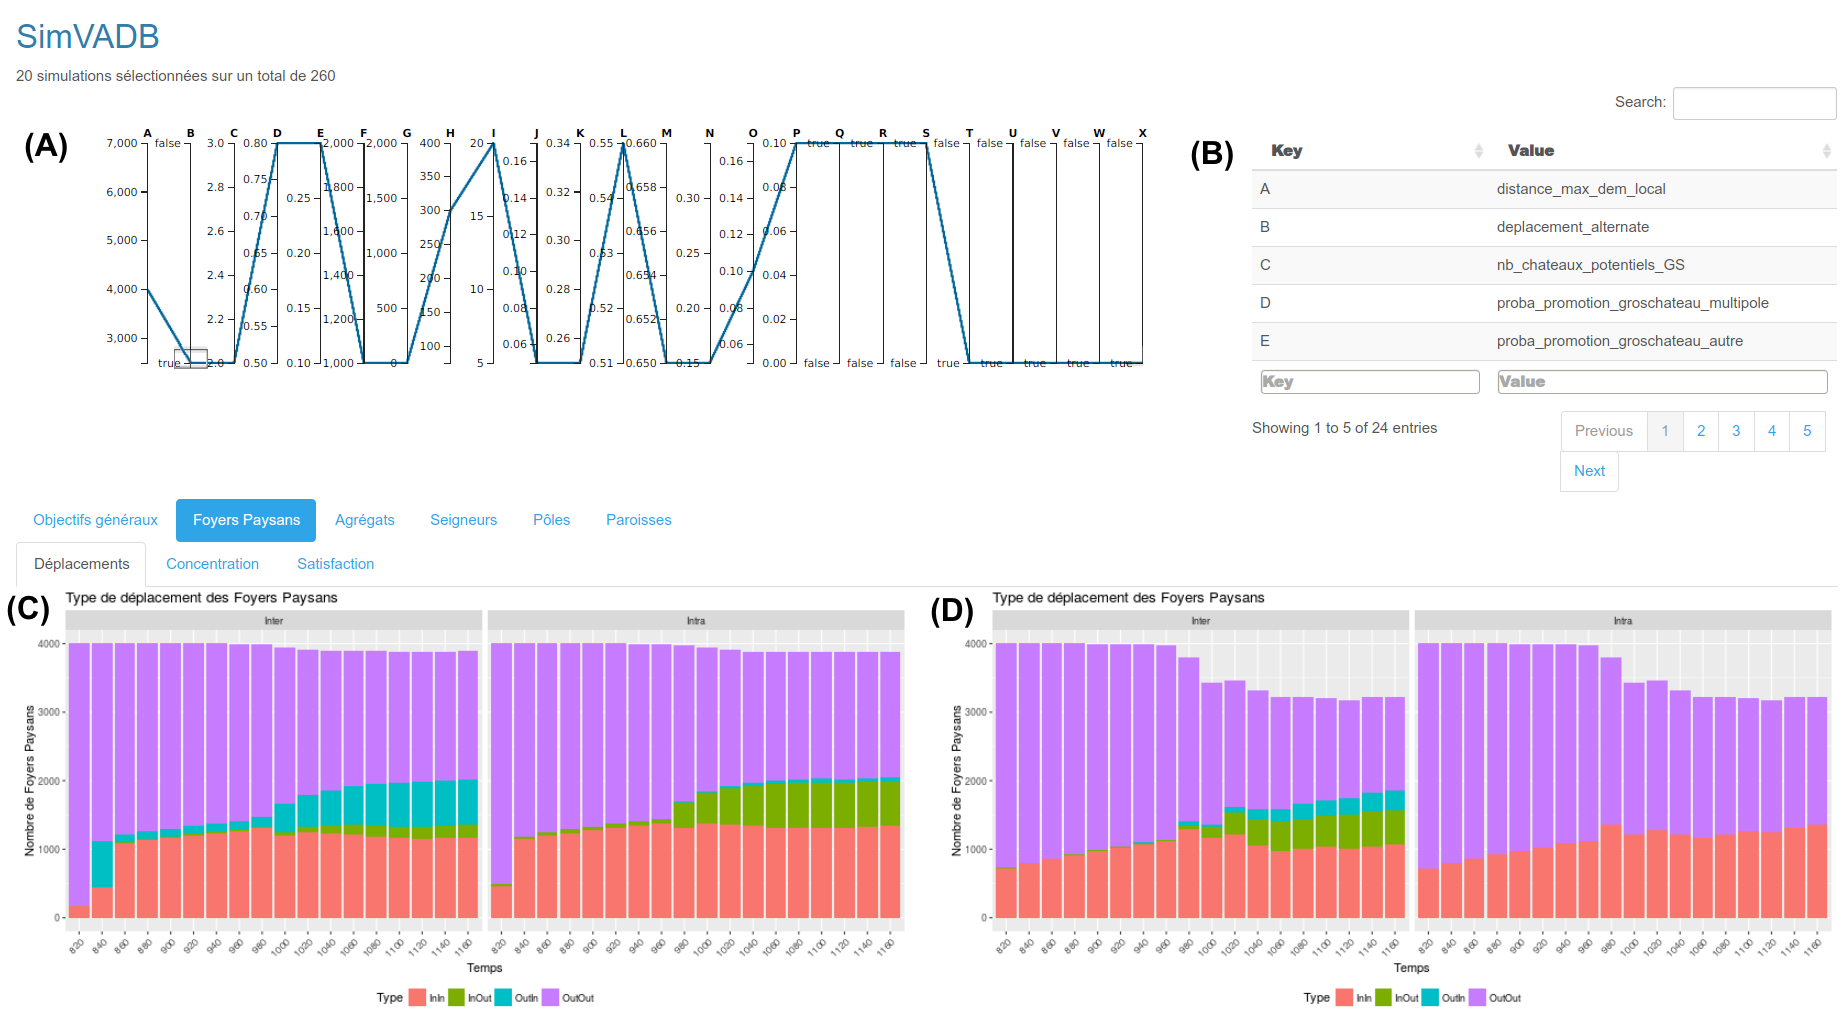
\includegraphics[width=\linewidth]{img/SimVADB_Dashboard2_annote_retouche.png}
		\caption{SimVADB (Simulation Visual Analysis DashBoard), un \textit{dashboard} d'exploration visuelle des indicateurs de sortie de simulation de SimFeodal.\\
		La sélection des simulations à explorer se fait dans le graphique en coordonnées parallèles (\textbf{A}), en \og brossant\fg{} des filtres graphiques sur les \og dimensions\fg{} du graphique, dimensions dont les intitulés sont explicités dans le tableau \textbf{B}.
		Les graphiques \textbf{C} et \textbf{D} indiquent l'évolution des types de déplacements des foyers paysans au cours des simulations.\\
		- Le graphique \textbf{C} représente, pour cet indicateur, une moyenne de l'ensemble des simulations intégrées dans la base de données (260 ici), recouvrant donc plusieurs valeurs de paramètres.\\
		- Le graphique \textbf{D} représente cet indicateur calculé depuis un sous-ensemble de 20 simulations (donc une expérience composée de 20 réplications), pour lesquelles le paramètre \og \textsf{B} \fg{} (\textsf{deplacement\_alternate}) vaut \textsf{true}.}
		\label{fig:simvadb_dashboard}
	\end{figure}

	Afin de permettre aux utilisateurs de remarquer les particularités des simulations explorées, nous avons choisi de mettre en emphase les différences entre la tendance générale des indicateurs, en calculant des moyennes de l'ensemble des simulations (\cref{fig:simvadb_dashboard} - \textbf{C}), et les valeurs spécifiques des indicateurs de l'expérience choisie (\cref{fig:simvadb_dashboard} - \textbf{D}).
	Cela permet, visuellement, d'être en mesure d'évaluer les sorties de simulation d'une expérience tout en ayant un référentiel visible.
	Les différentes expériences produisent des résultats sensiblement similaires\footnote{
		Si chaque expérience, et chaque réplication, produisent des résultats uniques, le choix d'une évaluation par des indicateurs visuels peut prêter à confusion si l'on n'a pas de repère précis.
		Les critères attendus, présentés dans \hl{le chapitre 3} sont ainsi assez précis pour départager une simulation très éloignée des attentes et une autre simulation plus conforme.
		Pour autant, par exemple quand les valeurs de paramètres varient faiblement, les résultats produits peuvent être assez similaires dans les grandes tendances qu'ils font ressortir.
	}, et on ne peut alors plus les comprendre sans les confronter à d'autres résultats similaires.
	Le choix d'une agrégation de l'ensemble des simulations effectuées est discutable, en ce qu'on aurait par exemple pu plutôt isoler des simulations \og de référence \fg{} afin de diminuer l'effet \og d'aplatissement \fg{} engendré par l'agrégation de résultats nombreux et hétérogènes.
	Toutefois, la variabilité des résultats étant encore assez restreinte, au moment de la création et de l'utilisation de SimVADB, ce référentiel agrégé permettait déjà une compréhension plus fine des sorties de simulations, en particulier dans l'analyse de l'impact de variations fines de valeurs de paramètres.

	\subsection{Explorer en comparant : SimEDB}\label{subsec:explorer-simedb}

	Après un travail de paramétrage grossier qui permet de stabiliser les mécanismes, il est souvent nécessaire de passer à une phase plus fine.
	On vise à ce moment à mieux calibrer un modèle à l'aide de variations de valeurs de paramètres de granularité inférieures.
	En vue d'évaluer les simulations, et donc de les différencier les unes des autres à l'aune des indicateurs générés, la comparaison d'une expérience spécifique avec un référentiel constitué de toutes les expériences précédentes ne permet plus de mener ce travail de comparaison fine.
	Les variations entre simulations sont trop fines pour être distinguables les unes des autres par le biais d'une comparaison avec un référentiel unique\footnote{
	On peut prendre l'exemple de SimFeodal.
	En faisant varier le nombre de foyers paysans de $4000$ à $4200$ ($5\%$ de variation), les résultats du modèle changent peu : de faibles variations de valeurs de paramètres entraînent le plus souvent de faibles variations dans les indicateurs de sorties observés.
	On peut de plus noter que les répercussions d'un changement de valeur de paramètre peuvent être très différentes de l'ordre de grandeur de ce changement de valeur.
	Cela s'explique par la non-linéarité de l'influence des paramètres.
	Dans l'exemple pris, pour ces $5\%$ de variation dans le nombre de foyers paysans, la majorité des indicateurs variera ainsi de moins de $1\%$.
	}.
	Cela s'entend quelque soit la manière dont ce référentiel est constitué, qu'il résulte d'une agrégation de simulations ou encore d'une version \og de base\fg{} du modèle (par exemple, dans le cas de SimFeodal, les versions principales identifiées dans le \hl{chapitre 4}).
	

	Pour pouvoir correctement évaluer les apports d'un nouveau jeu de valeurs de paramètres, et donc, dans une démarche itérative, pouvoir différencier deux expériences successives, il est nécessaire d'être en mesure de comparer directement les expériences les unes avec les autres, ou encore avec un référentiel facilement ajustable.
	On peut énumérer les quelques exemples de cas de figure suivants :
	\begin{itemize}
		\item Comparaison entre une expérience spécifique et une autre expérience spécifique de même \og importance\fg{}.
		Par exemple, comparer deux expériences qui font varier légèrement différement une valeur de paramètre.
		\item Comparaison entre une expérience spécifique et une autre expérience spécifique d'\og importance\fg{} différente.
		Cette différence de niveau peut être constituée par exemple par une version \og de base\fg{} que l'on comparerait à une variante de celle-ci.
		\item Comparaison entre deux expérimentations, par l'agrégation de leurs résultats.
		Si l'on a mené des expérimentations faisant varier de manière systématique deux paramètres différents, il peut être intéressant de les comparer en bloc, c'est-à-dire par exemple en prenant les moyennes de chacune des expériences composant ces expérimentations.
	\end{itemize}
	
	Ce faisant, on fait en fait varier la notion de \og simulation de référence\fg{}, qui peut alors revêtir plusieurs formes.
	Pour cela, il n'est plus possible de mener une comparaison visuelle entre un référentiel commun et une expérience spécifique, mais bien de baser l'évaluation sur la comparaison entre deux ensembles spécifiques qui doivent pouvoir être spécifiés.
	D'un point de vue méthodologique, cela requiert de pouvoir afficher conjointement les indicateurs de sorties de deux expériences (ou ensembles d'expériences).
	Cela implique aussi de laisser à l'utilisateur la responsabilité d'un choix supplémentaire puisqu'il faut désormais effectuer deux sélections : une pour chacun des points de comparaison.
	La sélection d'une expérience via l'usage de \textit{brushing} sur un graphique en coordonnées parallèles des valeurs de paramètres ayant montré son efficacité, il a été choisi d'étendre ce principe d'interactivité au choix du référentiel.
	
	Dans cette version remaniée de la plate-forme d'exploration (voir \cref{fig:simedb_villages}), renommée SimEDB\label{par:introduction-nom-simedb} (\textbf{Sim}Feodal \textbf{E}xploration \textbf{D}ash\textbf{B}oard)\footnote{
		\label{ftn:origine-simedb}
		La plate-forme d'exploration SimVADB (SimFeodal Visual Analysis Dashboard) a été renommée SimEDB ([...] Exploration Dashboard) par soucis de simplicité, le terme \og Exploration\fg{} nous semblant plus compréhensible et explicite que celui de Visual Analysis.
		Ce nom apporte de plus une cohérence sémantique entre plusieurs productions de l'auteur -- TimeLineEDB - \autocite{cura_timelineedb_2017}; RoadTrafficEDB et CitiBikeEDB - \autocite{cura_making_2017}.
		Cela inscrit cette plate-forme d'exploration de données issues de simulation dans une \og famille \fg{} d'outils d'exploration de données spatio-temporelles.
	}, l'accent est mis sur la comparaison de deux ensembles de résultats, chacun répondant à une sélection propre.
	L'utilisateur doit ainsi \og paramétrer\fg{} interactivement, via \textit{brushing}, les expériences à afficher pour le référentiel et pour les expériences à comparer.
	On dispose pour cela de deux outils de filtrage des simulations (partie de gauche dans la \cref{fig:simedb_villages}), qui peuvent être utilisés de concert, pour comparaison visuelle, ou par étapes successives\footnote{
		En menant par exemple une première comparaison entre une expérience \og A\fg{} en haut et \og B\fg{} en bas, puis en sélectionnant \og C\fg{} en haut, puis \og D\fg{} en bas etc.
		On compare ainsi A avec B, puis B avec C, et enfin C avec D.
	}.

	En superposant les graphiques et tableaux des indicateurs, la comparaison visuelle est facilitée.
	On peut alors comparer deux variations fines d'un mécanisme du modèle, en sélectionnant par exemple une unique différence dans les valeurs de paramètres du modèle (par exemple un paramètre relatif à la promotion des paroisses dans la \cref{fig:simedb_villages}).
	De manière générale, ce choix d'outil d'interrogation des données permet de répondre à l'ensemble des cas de figures identifiés dans les paragraphes précédents.
	
	\begin{figure}[H]
		\centering
		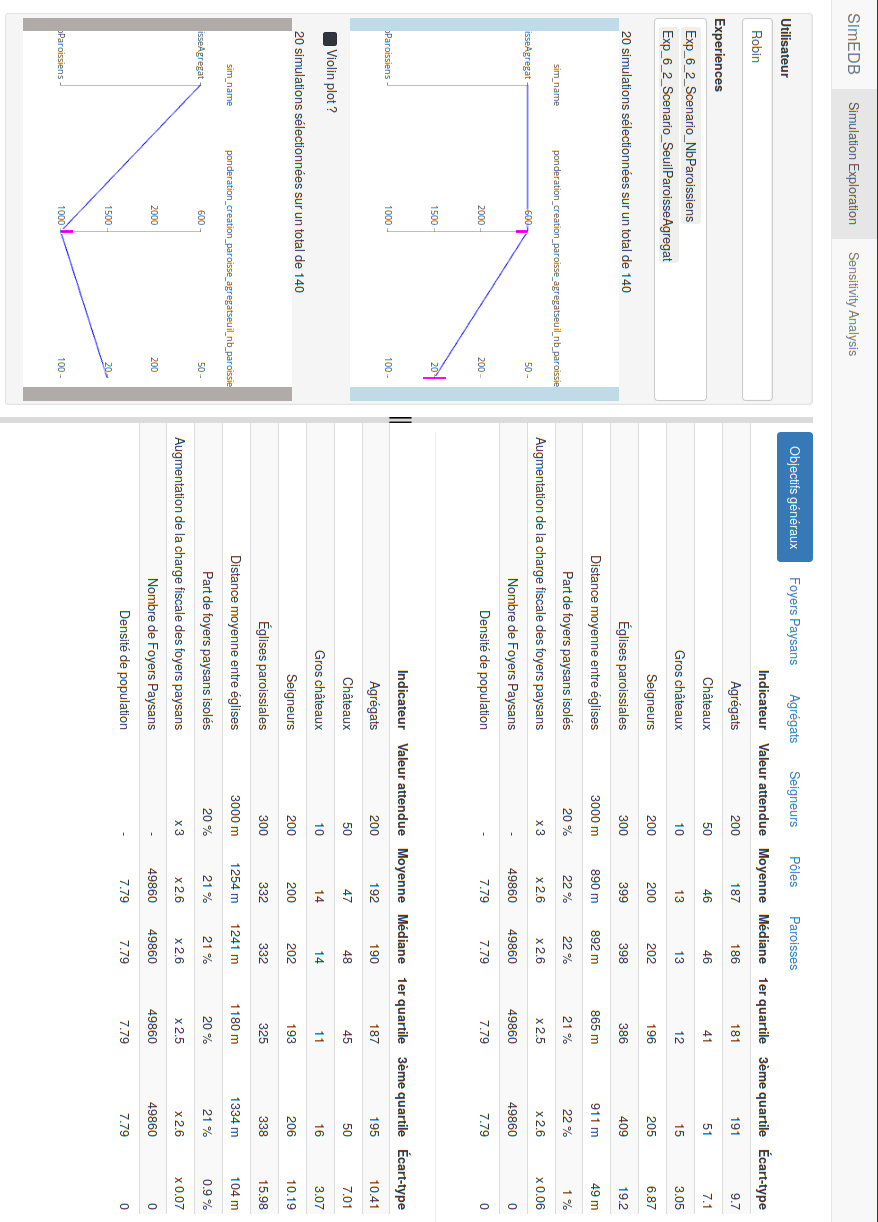
\includegraphics[width=\linewidth]{img/SimEDB_base_rotate.png}
		\caption{SimEDB }
		\label{fig:simedb_villages}
	\end{figure}

	\paragraph*{}
	Nous reviendrons plus précisément et longuement sur la description de SimEDB dans les parties suivantes (\cref{sec:SimEDB}, p. \pageref{sec:SimEDB}), mais après en avoir décrit les étapes de construction et les besoins auxquelles ces évolutions répondaient, il est maintenant nécessaire de revenir sur les données manipulées par cette plate-forme d'exploration.
	Le type, la structure et la masse de ces données (\cref{sec:sorties-simfeodal}) sont en effet indissociables des choix méthodologiques effectués pour SimEDB.
	Il est donc important de présenter les choix et contraintes de ces données avant d'entrer dans une description approfondie de la plate-forme.


%\setcounter{section}{2}
%\clearpage
\section{Organiser les données}\label{sec:organiser-donnees}

On a vu dans la première partie de ce chapitre (\cref{sec:sorties-simfeodal}) que les données produites par SimFeodal étaient nombreuses, diverses et massives.
La seconde partie (\cref{sec:explorer-sorties-simfeodal}) a montré les types de problèmes que de telles données, une fois exploitées pour en tirer les indicateurs de sortie, peuvent poser en matière d'exploration.

Nous souhaitons ici revenir sur une corollaire indispensable à l'utilisation efficace de ces données.
De la même manière que la multiplicité des indicateurs, des expériences et des expérimentations requiert des outils d'exploration adaptés, la multiplicité des données requiert des outils de stockage et d'interrogation eux aussi adaptés.
Là encore, on peut noter une succession de contraintes liées à ces données et à leur massification, contraintes qui limitent et guident les modes d'organisation de ces données.
Sans structuration adéquate, l'acquisition, l'archivage, l'interrogation ou encore la sauvegarde des données générées par le modèle ne peuvent être garantis, et encore moins de manière efficace.
Le choix d'une méthode d'organisation des données en sortie de simulations ne relève donc pas d'une quelconque coquetterie technique.
Au contraire, conditionne et contraint fortement aussi bien les modalités de création des indicateurs que les possibilités de la plate-forme d'exploration de les afficher de manière interactive.

%
%Contrairement à des modèles de simulations plus \og KISS \fg{}, par exemple les \og modèles-jouets\fg{} courants en Sciences Humaines et Sociales (\hl{ref Schelling/Sakoda, SugarScape, Prey-Predator, }), SimFeodal fait ainsi interagir de nombreux types d'agents, chacun doté de sorties spécifiques. Ces modèles sont le plus souvent évalués \og en direct\fg{}, les indicateurs présents dans l'interface des plate-forme de simulations suffisant à leur compréhension.
%La démarche suivie pour l'évaluation de SimFeodal repose sur des indicateurs visuels, qui doivent être examinés \textit{a posteriori} de leur production (\cref{subsec:observation-a-posteriori}), et l'évaluation du modèle ne peut être réalisée qu'en s'appuyant sur une part importante de ces sorties.
%
%Dans les modèles plus complexes utilisés en géographie (\hl{SimPop, MobiSim, SimPopLocal, MARIUS}), les données peuvent être plus massives (que ce soit intrinsèque au modèle (MobiSim) ou à sa méthode d'exploration (SimPopLocal)), mais leur structuration, souvent mono-agent, reste simple.
%Pour SimFeodal, où les indicateurs s'appuient parfois sur des requêtes croisant plusieurs types d'agents, la question de la structuration de ces données revêt une importance cruciale.




\subsection{Assurer la capacité d'interrogation des données}\label{subsec:capacite-interrogation}

Avant de se soucier du \og schéma\fg{} de la base de données\footnote{
	On utilise souvent le terme de \og schéma\fg{} pour désigner la version implémentée, dans un SGBD spécifique, du Modèle Conceptuel de Données (MCD).
	Contrairement au MCD, qui donne une version conceptuelle et générique d'une base de données, le schéma est donc tributaire du SGBD dans lequel il est intégré.
}, du choix du Système de Gestion de Base de Données (SGBD), ou encore des performances de ce dernier, il convient de se fixer sur la manière dont on souhaite entreposer les données.

De la myriade de fichiers issus de tableurs organisés dans une multitude de dossiers spécifiques à l'entrepôt de données décentralisé orienté documents, en passant par les traditionnelles bases de données relationnelles, les possibilités de stockage et d'organisation des données issues de simulations sont ainsi innombrables.
Plusieurs contraintes successives permettent de limiter le choix à un sous-ensemble de solution adaptées parmi lesquelles on peut alors mener une étude plus approfondie, passant notamment par des comparaisons entre ces candidats.

Une des premières contraintes est constituée par la nécessité d'interroger fréquemment et de manière répétée les données.
C'est l'une des contre-parties du passage d'un rapport automatique à un outil d'exploration interactif (\cref{subsec:dashboards}).
Ainsi, dans un rapport automatique, on interroge une fois les données pour en tirer les indicateurs de sortie, et ceux-ci ne sont plus amenés à changer, sauf re-calcul par exemple suite à des ajouts d'indicateurs.
Au contraire, dans un outil interactif, les indicateurs sont calculés depuis les données \og à la volée\fg{}, c'est-à-dire à chaque qu'un indicateur doit être affiché.
On peut mettre en place un système de cache, pour conserver les calculs déjà effectués, mais avec les dernières itérations de SimEDB où le nombre de possibilités de sélections est extrêmement important, ce n'est plus possible.
Il est nécessaire de procéder aux calculs à chaque affichage des graphiques et tableaux de résultats.
L'interrogation des données est donc extrêmement fréquente et répétitive.
Elle doit alors être aussi simple (en termes de mode d'interrogation) qu'efficace (en termes de rapidité d'interrogation).

Dans le cadre des données issues de SimFeodal, en vue de leur mobilisation dans SimEDB, nous avons ainsi eu à sélectionner quelques SGBD candidats parmi une foule de solution possibles.
Afin de guider ce choix, trois critères ont été définies, et forment, selon une hiérarchie propre à leur ordre, un ensemble de filtre ayant permis la réduction des SGBD possibles à un nombre appréhendable.
Ces critères, dont l'énonciation guidera cette partie, sont ainsi (1) l'universalité, ou \og agnosticité\fg{}, des SGBD aux outils de requête ; (2) la pérennité et stabilité des solutions disponibles et (3) les performances des SGBD considérés.

\subsubsection{Interroger de manière universelle et indépendante}

Lors de la conception d'un outil faisant appel à des données, qui plus est massives, il convient de se positionner tôt sur la manière d'interroger ces données.
Par interrogation, on entend ici, comme souvent dans le domaine des bases de données, la manière de faire appel, concrètement, aux données, pour en tirer les sous-ensembles, agrégations et autres résultats synthétiques résultant du traitement des données brutes.
Si l'on considère des données stockées dans un tableur, alors les \og formules \fg{}, les tableaux croisés dynamiques ou encore les graphiques issus du tableur sont des interrogations des données, qui s'expriment dans ce cas via un ensemble de langages, écrits -- les formules, qui font appel à des fonctions spécifiques des tableurs -- ou visuels -- les tableaux croisés dynamiques, construits en faisant glisser des intitulés de colonnes dans un tableau.

\paragraph*{Stockage distribué ou centralisé}\label{par:stockage-centralise}
Avant même de s'intéresser aux spécificités de ces langages, un premier choix réside dans le mode de stockage des données qui doivent être mis à disposition d'une plate-forme.
Doit-on laisser l'utilisateur intégrer lui-même les données, et ainsi, en faire un stockage \og distribué \fg{}, dans le sens où chaque utilisateur de l'application possèderait physiquement une copie locale des données ?
Ou, au contraire, les données doivent-elles être centralisées, c'est-à-dire enregistrées en une seule copie à laquelle les utilisateurs accèderaient à distance ?
Pour reprendre l'exemple des tableurs, doit-on privilégier une solution locale -- chacun ayant une copie du fichier tableur et menant ses propres modifications dessus -- ou une approche de type centralisée, par exemple en privilégiant des tableurs collaboratifs en ligne (\textit{Google Docs/Sheets} par exemple) ?

Habituellement, c'est-à-dire dans une grande majorité d'applications, les données sont stockées localement : cela permet, en particulier, de ne pas dépendre d'une connexion internet pour interroger des données qui seraient hébergées sur internet.
Dans le cas de SimFeodal, cette solution est rendue difficile, sinon impossible, par la masse de données en sortie de simulations.
Si chaque utilisateur de SimEDB devait posséder une copie des données, voir plusieurs en cas d'utilisations depuis différents ordinateurs, cela occuperait plusieurs gigaoctets de données à chaque fois.
De plus, en cas de mise à jour des données, c'est-à-dire d'insertions de nouvelles sorties de simulations, il faudrait distribuer à nouveau l'ensemble du jeu de données, à chaque fois.

Pour ces raisons, nous avons fait le choix d'un stockage centralisé, sous forme d'une architecture \og client-serveur\fg{}, hébergé sur un serveur internet dédié, ce qui permet à la plate-forme de travailler à chaque fois sur les données les plus à jour, réduit la taille du stockage physique associé, et dispense d'une configuration sur chaque poste utilisateur :
si le lien entre l'application et les données fonctionne correctement pour un utilisateur, il fonctionnera à l'identique pour tous les autres.
Ce choix présente un dernier avantage, non négligeable :
en stockant les données en un seul lieu, c'est-à-dire sur un serveur informatique, on peut faire en sorte de rendre ce serveur aussi performant que possible, et accélérer ainsi l'interrogation des données pour tous les utilisateurs.

\paragraph*{Interrogation spécifique ou générique}\label{par:interrogation-generique}

De nombreuses solutions intégrées de gestion de données proposent leurs propres modes d'interaction avec les données, c'est-à-dire un langage spécifique permettant d'interroger les données contenues dans le système\footnote{
	Souvent, cette interrogation se fait par appel à des \textit{API} (\textit{Application Programming Interface}, ou Interface de Programmation Applicative en français).
	Ces interfaces sont propres à chacune des plate-formes, et demandent donc un langage et un formalisme de requête spécifique.
}.
Au contraire, les SGBD les plus classiques s'appuient plutôt sur des langages de requêtes aussi standardisés que possibles, afin de faciliter l'adoption de leur propre solution à des utilisateurs d'autres plate-formes.
La spécificité présente l'avantage de langages plus adaptés aux données manipulées, et donc souvent plus intuitifs dans l'interrogation des spécificités des données.
De plus, la spécificité permet aussi une optimisation des requêtes, et est donc souvent plus performante que les solutions plus génériques.

De manière générale et dans le cas de SimFeodal, nous avons préféré privilégier une approche plus générique, faisant appel à des solutions de SGBD plus standardisées.
La raison tient principalement à une volonté de généricité du stockage des données : au cours des différentes étapes de construction de SimFeodal, les besoins en matières d'interrogation des données ont évolué.
Cette évolution était prévisible et prévue, et nous avons donc choisi dès le départ d'adopter uniquement des solutions modulaires, garantissant une évolutivité facilitée de la base de données, aussi bien regardant sa structure (enregistrement de nouvelles variables ou de nouveaux agents du modèle) que son contenu (massification des données en sortie au fur et à mesure de l'exploration du modèle).

De plus, dans la perspective de ce travail de thèse, où l'on cherche à rendre les productions aussi reproductibles et génériques que possible, il était indispensable de disposer d'un SGBD aussi standard que possible pour en faciliter l'adoption et l'adaptation à d'autres modèles de simulations par exemple.

\paragraph*{Bases de données relationnelles ou NoSQL}\label{par:sql-nosql}

Même une fois arrêté sur le choix de ne faire appel qu'à des outils standards pour stocker les données, le nombre de solutions disponibles demeure très important.
Afin de réduire ce nombre, on peut déjà choisir les grands types de SGBD auxquels faire appel.
Les SGBD sont ainsi souvent classés selon les grands traits de la méthode dont ils organisent les données.
Les deux grands types\footnote{
	Il en existe d'autres, comme les SGBD orientés objets (quasiment disparus aujourd'hui), orientés graphes (Neo4j\ldots), les SGBD pensés pour le stockage et l'interrogation d'ontologies (\textit{Triplestores RDF}, interrogeables en langage SPARQL) ou encore les nouveaux SGBD de type \og NewSQL \fg{} (Apache Ignite, CockRoachDB\ldots) pensés pour une parallélisation massive des données. Ces types de SGBD ne correspondent toutefois pas du tout aux besoins identifiés pour SimEDB/SimFeodal, et sont en général dédiés à des problèmes et marchés de niches. Nous ne les décrirons donc pas plus en détail ici.
} sont les SGBD \og relationnels\fg{} et les SGBD \og NoSQL\fg{}.
Si la distinction est sujette à de très nombreux débats, souvent virulents
\footnote{
	À l'instar des violentes querelles qui agitent régulièrement les informaticiens : Vim vs Emacs, Programmation Orientée-Objet vs Programmation Fonctionnelle, R vs Python\ldots
}
, on se contentera ici de définir les SGBD relationnels comme les SGBD, les plus fréquemment utilisés, où l'information est stockée dans des tables composées de champs -- les colonnes, correspondant aux variables -- et de lignes -- les entités décrites par les variables.
Le format des données est donc rectangulaire et n'accepte pas, comme dans un tableau statistique, que les entités possèdent un nombre de variables différent, ou encore des types de valeurs différents de celles des autres entités (une même colonne ne peut donc contenir conjointement un nombre et un texte dans des lignes différentes).
On nomme ces bases de données relationnelles via la manière qu'elles ont de faire communiquer des éléments hétérogènes, et donc contenus dans des tables différentes : si les tables ont une colonne en commun, on pourra alors effectuer une opération de jointure permettant de mettre en commun les informations de ces tables dans une unique table résultante.

A l'inverse, les SGBD NoSQL se définissent de manière opposée à ce mode de stockage\footnote{
	À l'origine, c'était le sens fort du nom \og NoSQL \fg{} : Non SQL, le SQL faisant ici références aux SGBD pré-existants, majoritairement relationnels, dont la mouvance NoSQL, portée par l'apparition des \og \textit{big data} \fg{} a voulu se distinguer.
	Sans entrer dans le détail, notons tout de mêmes que de nombreux SGBD NoSQL, qui traduisent désormais cet acronyme par \og Not only SQL\fg{}, sont maintenant relationnels, mais mettent en avant d'autres types d'approches.
}, rompant par exemple la contrainte d'unicité de type des colonnes, ou de nombre identique de colonnes renseignées pour chaque entité. Pour simplifier le discours, on se contentera de caractériser les SGBD NoSQL comme des SGBD non relationnels.
Les SGBD NoSQL ont, en général, de bien meilleures performances et une plus grande flexibilité que les SGBD relationnels.
Dans le cas de SimEDB/SimFeodal, où l'on est confronté à des données massives, cela présente un avantage non négligeable.

Toutefois, leur flexibilité est associée à une contrainte majeure en termes de généricité : alors que les SGBD relationnels partagent un langage d'interrogation commun, le SQL (\textit{Structured Query Language})\footnote{
	Ce langage d'interrogation est omniprésent dans l'interaction avec les SGBD, mais aussi, avec de légères variantes, au sein de nombreux logiciels reposant des sélections de données, par exemple les logiciels SIG qui se basent sur la syntaxe du SQL (le fameux triptyque \texttt{\textbf{SELECT} \ldots~\textbf{FROM} \ldots{} \textbf{WHERE} \ldots})
}, les SGBD NoSQL font plus souvent appels à des langages spécifiques à chaque SGBD.
Pour SimEDB, cela impliquerait une fort dépendance au SGBD choisi : en cas de changement de SGBD, toutes les requêtes seraient à reformuler dans le nouveau langage, parfois même selon des logiques extrêmement différentes les unes des autres (dérivés du SQL, interrogations via des objets JSON, via des langages de parcours de graphes\ldots{}) etc.
Au contraire, avec les SGBD relationnels, le langage de requête étant commun, une fois le code d'interrogation généré, il est très aisé de changer de SGBD cible.
Cela garantie une forte capacité d'évolutivité aux outils d'interrogation de données tels que SimEDB.
Puisque les fournisseurs de données sont interchangeables, on peut en changer au fur et à mesure de l'apparition de nouveaux besoins.

En raison de la généricité de ces solutions relationnelles, qui vient s'ancrer dans la recherche de reproductibilité et de généricité de notre démarche d'ensemble, nous avons donc choisi de faire reposer le stockage et l'interrogation des données sur des SGBD relationnels.
Cette décision s'est montrée d'autant plus heureuse que, au cours de la construction et de l'évolution de SimEDB, le SGBD choisi pour héberger les données a changé plusieurs fois.
La généricité des outils choisis a permis de minimiser, voire quasiment d'éviter, les changements à apporter au code-source de SimEDB relatif à l'interrogation de données en vue de produire les indicateurs de sortie depuis les données brutes en sortie de SimFeodal.


\paragraph*{Entrepôts de données et interrogation directe}\label{par:interrogation-directe}

En parallèle des SGBD, des solutions \og intermédiaires\fg{} permettent de s'abstraire des SGBD en eux-mêmes pour mener les requêtes.
Ces solutions, que l'on nomme \og Entrepôts de Données\fg{} (\textit{Data Warehouses}), se comportent comme une surcouche faisant l'interface entre un ou plusieurs SGBD et la requête émise par le client final.
Elles se placent donc comme intermédiaire entre les SGBD mobilisés et les applications qui les interrogent.
Les entrepôts de données jouent aussi bien le rôle d'agrégateurs de données\footnote{
	C'est-à-dire qu'ils permettent d'agréger des sources de données composites, provenant potentiellement de différentes sources (plusieurs bases de données relationnelles) et de différents types de sources (différents SGBD, relationnels ou non par exemple).
} que d'environnements de manipulation et de restructuration de données (on les nomme alors \og ETL\fg{} -- \textit{Extract-Transform-Load}).

Le grand intérêt de ces outils d'interface est d'abstraire la complexité de chacune des bases de données manipulées en générant une interface d'interrogation unique et générique, souvent performante grâce à des optimisations spécifiques (pré-calcul des requêtes possibles par exemple).

\hl{Dans les paragraphes suivants, Lena note qu'elle a perdu le fil mais que c'est bien écrit.}

Dans le domaine de la visualisation interactive de données, ces outils sont beaucoup utilisés, en particulier dans le monde de l'informatique décisionnelle.
Ils se révèlent en effet extrêmement utiles quand les données sources ne peuvent être modifiées (par exemple quand elles sont issues de chaînes de collecte complexes, ou encore quand leur volumétrie et leur débit est important), puisqu'ils permettent de constituer une surcouche rendant l'interrogation et la visualisation de ces données accessibles à des analystes non spécialistes de la manipulation de données.
Toujours en informatique décisionnelle, il est courant de faire appel à des entrepôts de données d'un type spécifique, les \og traitements analytiques en lignes\fg{}, ou environnements OLAP (\textit{\textbf{O}n\textbf{L}ine \textbf{A}nalytical \textbf{P}rocessing}), qui permettent de structurer, par exemple sous formes de cubes de données, des sources de données hétérogènes présentant de nombreuses dimensions.

Les environnements OLAP ont été utilisés, promus et adoptés dans le champs scientifique de la géomatique, en ce qu'ils permettent de mettre en place rapidement des environnements d'analyse visuelle de données multi-dimensionnelles spatiales et temporelles.
Dans ce cadre, où ces outils sont appelés \og SOLAP\fg{} (\textit{Spatial OLAP}), les données spatiales s'intègrent extrêmement bien en raison de leur capacité à s'emboîter selon les échelles, ouvrant dès lors la voie à des analyses multi-échelles et multi-dimensionnelles complexes.

Dans la communauté géomatique francophone, les solutions SOLAP sont bien représentées (par exemple autour de Sandro Bimonte et de son travail de visualisation de données spatiales environnementales,  \autocite{bimonte_integration_2007, bimonte_towards_2005, zaamoune_new_2013}, et sont couramment employées pour répondre à des questionnements méthodologiques proches de ceux développés dans cet ouvrage.
En lien avec les besoins de performances identifiés plus haut, on notera que certaines solutions OLAP permettent aussi d'optimiser la vitesse d'interrogation de bases de données, et visent ainsi à garantir une réponse rapide pour des outils d'interrogation de données interactifs \autocite{zeng_iolap_2016}.

Nous avons cependant choisi de ne pas faire usage de ces outils pour les mêmes raisons que pour les SGBD NoSQL : les avantages qu'ils présentent ne suffisent pas à contre-balancer les défauts en termes de généricité qu'ils introduisent. Pour profiter au mieux de ces environnements, il est en effet nécessaire de faire appel à un nouveau langage d'interrogation des données (le \og MDX\fg{}, de \og \textit{Multidimensional Expressions}\fg{}).
Les différentes solutions OLAP/SOLAP, de plus, présentent les mêmes inconvénients que les SGBD NoSQL : chacune interagit de manière propre aux différents SGBD, et ces outils sont donc difficilement interchangeables.

De la même manière, on se restreindra, parmi les SGBD relationnels interrogeables en SQL, à ceux qui disposent d'une méthode d'interrogation standard : si tous ces SGBD acceptent le SQL, certains demandent par exemple des protocoles spécifiques pour recevoir établir la connexion au SGBD, recevoir la requête et renvoyer les données correspondantes.
Pour ce même choix \og d'agnosticité \fg{} de la plate-forme d'interrogation face à la solution de stockage choisie, on ne conservera que les SGBD acceptant les connexion standardisées (ODBC et JDBC).

\paragraph*{SGBD et données spatiales}\label{par:sgbd-spatial}

On a mentionné le fait que les entrepôts de données étaient fortement utilisés, en particulier dans la communauté géomatique, car très appropriés aux données spatiales.
De prime abord, ce point peut paraître critique : jusque là, on s'est contenté de mentionner les capacités organisationnelles de SGBD, et non leur aptitude à manipuler des données spatiales.
Ce point, dans les SGBD relationnels, constitue un filtre important : sur la centaine de solutions disponibles, seule une poignée est en mesure de stocker efficacement et d'interroger de l'information spatiale \footnote{
	Les données spatiales peuvent être stockées dans tous les SGBD si l'on attribue une représentation textuelle, en chaînes de caractères, par exemple en utilisant le format \textit{Well-Known Text} (WKT).
	Pour autant, ce format est lourd, inadapté à une indexation, et ne peut permettre à un SGBD de mener des requêtes spatiales directement depuis ces entités.
	Il est ainsi, par exemple, impossible de calculer le centroïde d'un polygone directement depuis une représentation WKT, alors que c'est aisé avec un stockage géométrique.
}.

Pourtant, au regard des indicateurs de sortie de simulation sur lesquels on s'appuie pour évaluer le comportement de SimFeodal, une grande majorité est non spatiale, en raison de la difficulté à agréger des données spatiales théoriques.
Dans SimFeodal, la plupart des indicateurs de sortie sont non spatiaux, c'est-à-dire qu'ils mobilisent plus la dimension attributaire des données que leur dimension géographique\footnote{
	Les raisons en sont multiples et on y reviendra largement dans le \hl{chapitre 7}.
	Notons tout de même que les indicateurs résultent de l'agrégation des réplications, et que cette agrégation est extrêmement complexe sinon impossible sur des données spatiales majoritairement aléatoires (voir \hl{chapitre 2, section 2.2.2.1}).
}.

La gestion de données spatiales ne constitue donc pas une absolue nécessité, contrairement aux points évoqués auparavant.
Elle peut toutefois se révéler avantageuse, ne serait-ce que pour permettre l'observation des configurations spatiales simulées.
Cela constitue une approche idiographique, visant à exemplifier plus qu'à synthétiser, mais permet tout de même une compréhension rapide des changements de structures spatiales.
Toutes choses égales par ailleurs, on privilégiera donc des solutions de stockage ayant une capacité à gérer les données spatiales.

\paragraph*{}
Pour héberger et organiser les données produites par SimFeodal, en vue de leur interrogation dans SimEDB, nous avons choisi de restreindre la myriade de solutions disponibles grâce à plusieurs filtres successifs.
En premier lieu, on a choisit de faire appel à des solutions centralisées (\nameref{par:stockage-centralise}), au sein de Systèmes de Gestion de Base de Données (SGBD).
Ces SGBD permettent une interrogation standardisée (\nameref{par:interrogation-generique}) via un langage de requête universel, le SQL (\nameref{par:sql-nosql}).
On a ensuite décidé d'interroger ces SGBD sans passer par l'intermédiaire d'entrepôts de données, et au travers de connexion aussi standardisées que possible (\nameref{par:interrogation-directe}).
Les SGBD répondant à ces critères sont les SGBD \og relationnels \fg{}, dont certains possèdent qui plus est une capacité intéressante à stocker et interroger des données spatiales (\nameref{par:sgbd-spatial}), ce qui constitue notre dernier filtre.

\subsubsection{Interroger de manière robuste et efficace}\label{subsubsec:interroger-robuste-efficace}

En dépit de l'accumulation de critères exposée précédemment, une quantité importante de SGBD demeurent en lice.
Afin de les différencier, nous avons choisi d'ajouter des critères qui ne portent plus sur les grands types de SGBD, mais plutôt sur une différenciation des SGBD relationnels existants.
Ces deux critères, précisés par la suite, sont d'une part la robustesse des SGBD, et d'autre part leurs performances.
Ces critères sont pas des \og prétextes \fg{} à une hiérarchisation quantifiée des SGBD, mais ont une importance prépondérante dans notre cas d'utilisation.

\paragraph*{Robustesse des SGBD}
Le premier critère ajouté est celui de la robustesse, c'est-à-dire, ici, de la capacité du SGBD à être interrogé de manière (1) stable et  (2) pérenne dans le temps.
Une même requête sur les mêmes données doit systématiquement renvoyer le même résultat (stabilité), quelle que soit la durée séparant ces requêtes (pérennité).
Si la base de données n'est plus interrogeable quelques mois après sa configuration, ou qu'elle renvoie des résultats différents, alors elle ne peut constituer une solution crédible à l'exploration d'un modèle sur une période longue.

La \textbf{stabilité} des bases de données est principalement due à la manière de stocker l'information d'un point de vue informatique.\\
En premier lieu, l'information peut être contenue \og en clair\fg{} ou alors de manière archivée.
Un stockage \og en clair\fg{} est plus facilement accessible, puisqu'on peut le consulter avec n'importe quel éditeur de texte.
Un stockage archivé est moins universel, mais occupe généralement un espace disque inférieur et comporte des mécanismes de vérification de la cohérence des données.
Il est donc plus stable.\\
Une second différenciation tient à l'emplacement lieu du stockage.
Celui-ci peut être effectué dans un unique fichier, ce qui a l'immense avantage de la portabilité des données : pour faire migrer ou sauvegarder la base de données, il suffit de copier le fichier.
La plupart des SGBD adoptent toutefois un mode d'organisation en plusieurs fichiers, notamment pour des questions de redondance et de vérification de l'intégrité des données : en multipliant les fichiers, on minimise le risque d'erreur critique sur l'ensemble des fichiers à la fois.
On notera enfin un dernier type de SGBD, où l'information n'est pas stockée sur un disque dur, mais est entièrement contenue dans la mémoire vive de l'ordinateur : les SGBD \og \textit{in-memory}\fg{}.
Ces SGBD sont les plus rapides et stables, mais il faut les re-constituer à chaque redémarrage du serveur qui les héberge, ce qui peut prendre un temps important.

L'enjeu du choix est de se prémunir de \og corruptions\fg{} de la base de données : quand le SGBD ne comporte que pas ou peu de mécanismes de vérification de l'intégrité ou de la cohérence des données, il peut arriver qu'une base de données se corrompe.
On peut prendre l'exemple de l'exécution d'une requête demandant un calcul complexe et long.
Cette requête pourrait être interrompue en cours d'exécution par faute d'un \textit{bug} ou d'une expiration de sessions (\textit{timeout}). Dans ce cas, il se peut que la base de données s'arrête dans un état muté -- avec une nouvelle table ajoutée pour moitié par exemple -- et ne soit donc plus intègre.
C'est très fréquent pour les SGBD basés sur un unique fichier, ou encore stockés en clair, puisque les nouvelles informations de la base de données y sont ajoutées au fur et à mesure, plutôt que d'être intégrées dans un fichier annexe que l'on pourrait réinitialiser en cas d'erreur.\\
Avec la volumétrie des données produites par SimFeodal, les requêtes peuvent s'avérer très longues, et une erreur dans une requête peut fréquemment corrompre la base de données.
En termes de stabilité, on se tournera donc plutôt vers des SGBD relationnels stables, basés sur une redondance des données et donc sur des architectures archivées et multi-fichiers.


La \textbf{pérennité} des SGBD est un sujet proche, tenant aussi à la capacité à interroger les données contenues dans une base de données, mais cette fois-ci du point de vue de l'interrogation en elle-même plutôt de des données sur lesquelles elle s'applique :
si le SQL est un langage standard\footnote{
	Dans les faits, on notera tout de même qu'il existe plusieurs normes successives, des \og révisions\fg{} du SQL, qui apportent chacune leur lot de subtilités dans l'usage du langage.
	Les SGBD interrogeables en SQL ne disposent donc pas toutes des mêmes fonctionnalités, selon la révision du SQL qu'elles respectent.
}, les types de données intégrées varient cependant d'un SGBD à un autre (champs textuels ou d'entiers \og courts\fg{} par exemple).
SQL étant un langage typé, selon la manière (bas niveau) dont sont intégrées les données, certaines requêtes identiques peuvent renvoyer des résultats différents selon les SGBD.
Plus gênant, les normes implémentées peuvent varier d'une version à l'autre d'un SGBD.
Un SGBD relationnel respectant strictement la norme SQL pourrait ainsi évoluer pour supporter plus de fonctionnalités, par exemple en ajoutant des fonctions plus récentes (fenêtres glissantes, ajouts en masse etc.), et renverrait dès lors des résultats différents selon les versions.
Pour les SGBD les plus employés, le nombre d'utilisateurs garantit une rétro-compatibilité des requêtes.
Pour les SGBD de moindre envergure cependant, par exemple les plus performants et récents issus de la recherche en informatique, cette rétro-compatibilité n'est pas du tout garantie.

Comme souvent en matière d'infrastructure informatique, il est donc nécessaire de tenir compte d'un compromis entre l'ancienneté et la forte adoption de certains SGBD d'une part, et les facilités et gains de performances amenées par les plus récents d'autre part.
Dans le cas des données de SimFeodal, en tenant compte de cet inévitable compromis, nous avons choisi de privilégier des SGBD reconnus, soient-ils anciens et fortement adoptés ou plus récents mais utilisés par des acteurs d'envergure\footnote{
	La liste des solutions envisagées, ensuite comparées à l'aube de leurs performances, est visible dans l'axe des ordonnées de la \cref{fig:db-benchmarks}.
}.
Ce faisant, on se coupe immanquablement de solutions extrêmement intéressantes et performantes\footnote{
	Par exemple BlinkDB \autocite{agarwal_blinkdb_2013}, qui permet de limiter une requête à un temps maximal d'exécution donné : quand la requête n'est pas complète, le SGBD renvoi une estimation du résultat, estimation qui gagne en précision quand on augmente la limite temporelle.
	Un SGBD de ce type serait extrêmement précieux en \textit{visual analytics}, mais la jeunesse de cet outil ainsi que sa nature de projet de recherche rendent incertain la continuité de son développement dans le temps.
	En 2018, le projet semble d'ailleurs avoir été abandonné\ldots
}.
Ce choix est toutefois en la large faveurd'une meilleure garantie de pérennité, et de robustesse en générale, des données de SimFeodal.

\paragraph*{Performance des SGBD}

Une fois que les solutions disponibles ont été discriminées par leur type, par leur interface avec les requêtes et par leur robustesse, la quantité de SGBD restant demeure de l'ordre de la dizaine.
Pour choisir, parmi ceux-là, le SGBD qui sera le plus adapté aux besoins identifiés, il est donc nécessaire d'établir des critères plus précis et quantifiables.
Dans le cas d'une application interactive, c'est-à-dire où le nombre de requêtes émises au cours d'une session d'utilisation peut être importante, les performances des SGBD constituent un critère majeur pour départager l'ensemble des SGBD considérés.

Il est difficile de qualifier les \og performances\fg{} d'un SGBD : on entend en fait par ce terme un vaste ensemble hétérogènes de propriétés.
On peut par exemple juger les performances par le filtre de la mémoire occupée par le stockage d'une base de données, ou encore par le nombre de requêtes concurrentes que peut gérer un SGBD, ou encore par la capacité à paralléliser le stockage sur plusieurs serveurs.
Dans notre cas, ces points sont assez peu significatifs : en dépit de la quantité de sorties, l'ordre de grandeur -- quelques gigaoctets de données -- reste largement entreposable sur un environnement classique, sans besoin de parallélisation.
De la même manière, SimEDB est un environnement dédié à des utilisateurs experts, en petit nombre : les chercheurs travaillant autour de SimFeodal.
La quantité de requêtes simultanées ne peut donc pas dépasser la dizaine, ce qui constitue une trivialité pour l'ensemble des SGBD relationnels classiques.
On s'attachera donc à juger les performances en matière de rapidité d'exécution des requêtes.
Il ne s'agit pas ici de choisir un SGBD qui ferait gagner quelques millisecondes par rapport à un autre, mais plutôt de discriminer les SGBD présentant une durée de réponse trop importante pour notre usage.

En effet, plus les données sont massives, plus le temps d'exécution d'une requête augmente, souvent sous la forme d'une fonction puissance.
Si tous les SGBD présentent des vitesses acceptables et proches sur des bases de données de faible volume, l'écart s'accroît considérablement à mesure que les données s'accumulent.
La \cref{fig:db-benchmarks}\footnote{\label{ftn:dataset-exemple}
	Dans cette figure, on compare la rapidité de différentes requêtes sur un jeu de données identique selon les SGBD.
	Ce type de test de performance permettant la comparaison de solutions techniques diverses est appelé \textit{benchmark}.
	Ce jeu de données, composé de 100 Millions de lignes et de deux colonnes numériques, présente une volumétrie comparable (franchement inférieure en nombre de colonnes toutefois) à celle des données issues de SimFeodal qui sont interrogées dans SimEDB.
} montre les différences incontestables qui existent entre les SGBD étudiés. On peut y constater que l'écart est gigantesque, par exemple vis-à-vis du temps nécessaire à une jointure, entre les 4 secondes de MonetDB et les 300 secondes (5 minutes\ldots) de SQLite.
Le choix d'un SGBD selon ses performances a donc un impact majeur sur la fluidité d'une application d'exploration de données massives.
Pour départager les SGBD, on comparera leurs performances selon les différents types d'opérations demandées, qu'elles concernent l'écriture dans la base (insertion) ou des types de lecture (agrégation et jointure).

\clearpage
\subparagraph{Performances en écriture et en lecture}

La \cref{fig:db-benchmarks} affiche des résultats qui semblent globalement ordonnés (les quatre premiers SGBD sont par exemple quasiment toujours plus lents que les 2 derniers), mais fluctuent cependant à la marge selon les opérations demandées.
La première colonne du graphique montre ainsi le temps nécessaire à l'insertion du jeu de données exemple (voir la note de bas de page \ref{ftn:dataset-exemple}) dans le SGBD depuis un fichier CSV.
Les deux colonnes suivantes exposent le temps nécessaire au traitement d'une requête, donc à une interrogation des données une fois archivées dans les bases de données.
On peut constater que le classement des SGBD varie faiblement en lecture, et de manière assez faible en insertion : les deuxièmes et troisièmes colonnes respectent un ordre globalement similaire, assez différent de celui de la première colonne.
Dans un environnement classique, la performance d'insertion de données est un facteur prépondérant : quand de nouvelles données sont ajoutées constamment, par exemple pour stocker des données issues de capteurs automatiques, l'insertion peut vite constituer le goulot d'étranglement de la solution.

Pour SimFeodal, l'insertion n'est pas véritablement un enjeu : les données sont ajoutées par bloc, manuellement, une fois que des nouvelles simulations ont été exécutées.
C'est donc au pire un acte quotidien, mais dans ce cas, que la requête demande 10 secondes (MapD) ou 10 minutes (MySQL InnoDB), cela n'a que peu d'impact.
La première colonne est donc un indicateur de performance peu adapté dans notre cas.

Les deux colonnes suivantes, relatives à l'interrogation de données, se révèlent au contraire extrêmement importantes : à chaque action de l'utilisateur de SimEDB, une nouvelle requête est envoyée pour calculer un nouvel indicateur correspondant au jeu de données filtré manuellement (cf. \cref{subsec:explo-interactive}).
À chaque affichage d'onglet, une nouvelle requête est donc émise et traitée. Même si tous les indicateurs ne sont pas systématiquement mobilisés -- et donc calculés -- (cf. \hl{chap 3}), cela signifie tout de même que pour chaque sélection, une bonne dizaine d'indicateurs seront observés, et donc, autant de requêtes.
Quand une requête demande 60 secondes (par exemple PostgreSQL en \og jointure\fg{}), cela implique que chaque indicateur requiert au moins une minute avant de s'afficher.
Pour observer une dizaine indicateurs, l'utilisateur devra donc attendre patiemment une dizaine de minutes, sans même tenir compte du temps qu'il passera à les analyser visuellement.

Pour noircir le trait, notons de plus que les résultats communiqués dans la \cref{fig:db-benchmarks} correspondent à des requêtes simples qui ont valeur d'exemples de base.
Dans le cas de SimEDB, le calcul des indicateurs requiert des requêtes plus complexes, faisant appel à des agrégations et à des jointures en même temps, et les délais affichés dans ce \textit{benchmark} sont donc bien inférieures aux durées éprouvées en conditions réelles au sein de SimEDB.


\begin{figure}[H]
	\centering
	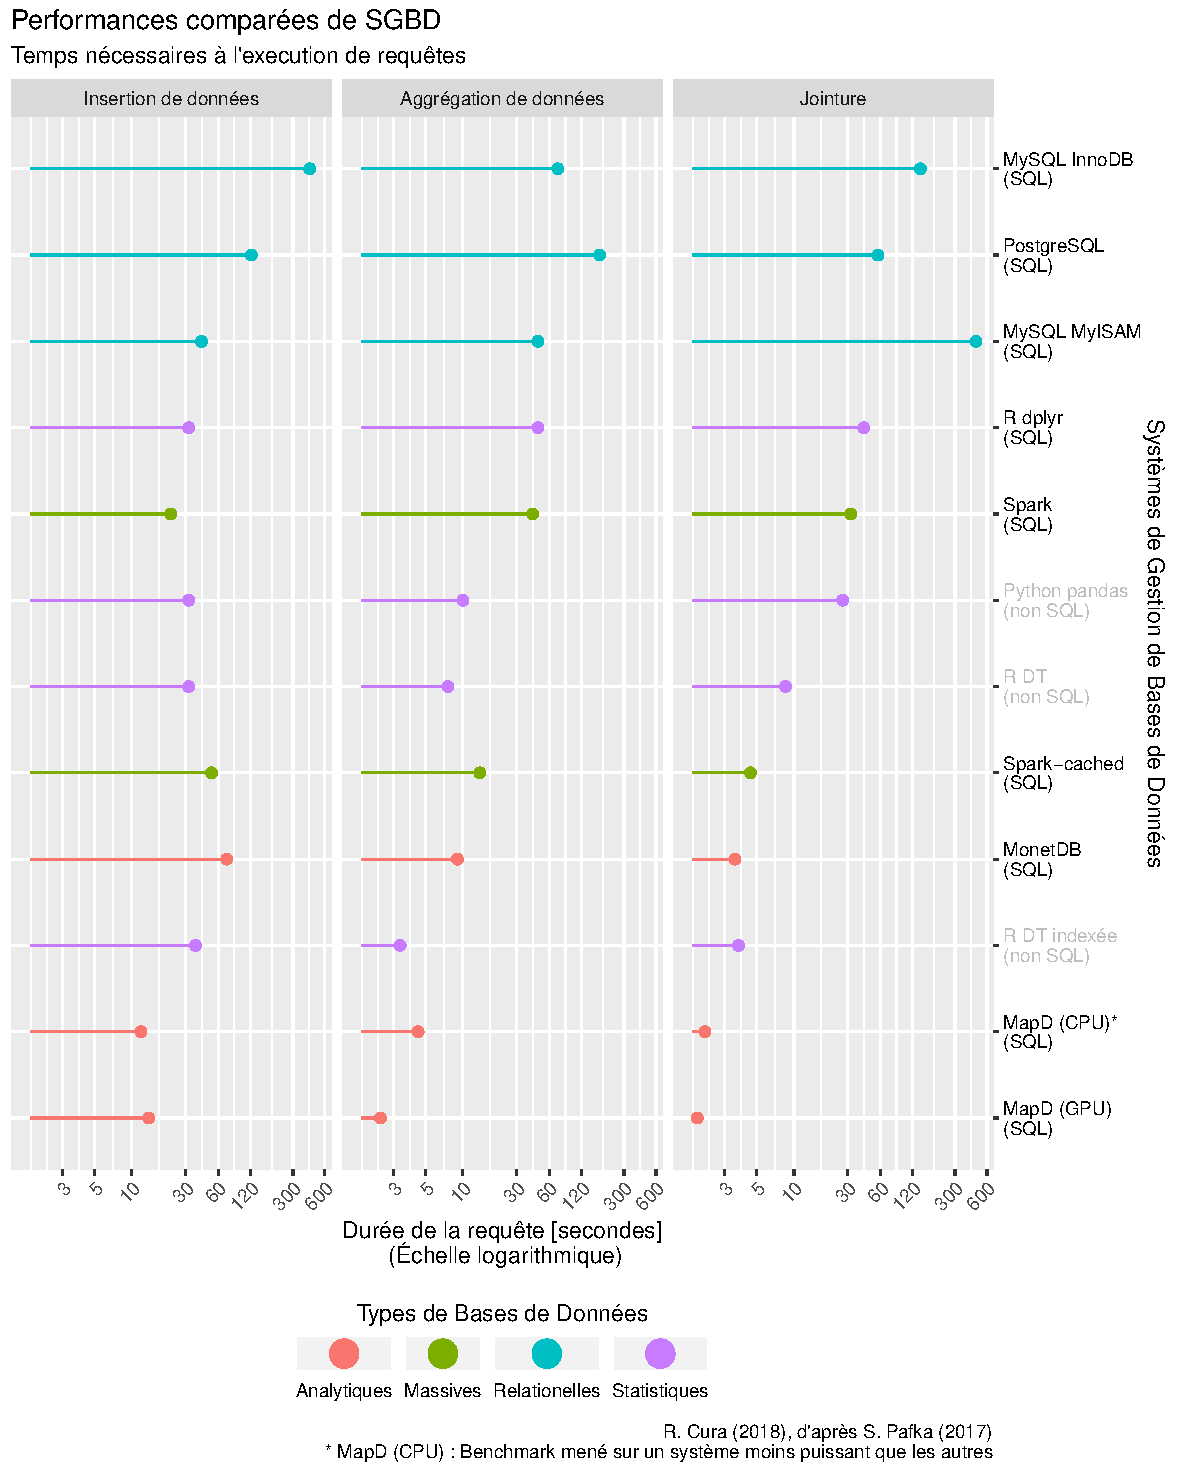
\includegraphics[width=\linewidth]{img/benchmark_results.pdf}
	\captionsetup{width=.95\linewidth}
	\caption[Comparaison de la performance de différents SGBD sur un jeu de données test de 100 millions de lignes.]{Comparaison de la performance de différents SGBD sur un jeu de données test de 100 millions de lignes. 
		Résultats tirés de \textcite{pafka_benchm-databases_2017} et complétés par l'auteur.\\
		Les \og types de Bases de Données\fg{} correspondent aux usages les plus fréquents des SGBD comparés :\\
		- Analytiques : SGBD optimisés pour les traitements de type agrégation, via une architecture orientée colonne plutôt qu'orientée ligne comme dans les SBGD Relationnels. Ils sont optimisés pour la rapidité d'exécution.\\
		- Massives : SGBD pensés pour la gestion et l'interrogation de données massives (big data), permettant notamment une parallélisation des requêtes. Ils sont optimisés pour la capacité à gérer des volumes gigantesques de données.\\
		- Statistiques : SGBD internes aux environnements de traitement de données statistiques, reposant sur une gestion en mémoire vive.
		Souvent intégrés d'office dans les environnements décrits (R, Python), ce sont les SGBD les plus simples à mettre en place et à manipuler.
	}
	\label{fig:db-benchmarks}
\end{figure}

\subparagraph{De l'intérêt de gagner quelques secondes}

La \cref{fig:db-benchmarks} permet d'isoler un sous-ensemble de quatre SGBD ayant, avec le jeu de données testé, des réponses inférieures à une dizaine de secondes : Spark avec cache, MonetDB et MapD sur CPU ou GPU.
On pourrait se contenter de choisir le SGBD le plus complet parmi ces quatre solutions.

Pourtant, un autre domaine d'étude appuie l'importance relative des écarts, mêmes faibles, dans les durées de requête.
Ce domaine est celui des sites internet, où les requêtes servent à générer le contenu de différentes pages en interrogeant des base de données de contenu.
La consultation d'un site internet consiste à charger plusieurs pages, pour l'utilisateur.
Du point de vue du serveur, chacune des pages demandées par l'utilisateur requiert différentes requêtes à des bases de données.
La navigation dans un site est donc assez comparable à l'utilisation d'une application d'exploration de données : des requêtes hétérogènes, plus ou moins lourdes, s'y succèdent et visent à filtrer et mettre en forme, de manière explicite, des extraits d'informations stockées dans des bases de données.
Plusieurs études ont montré que la durée d'affichage d'une page web jouait de manière considérable sur l'usage d'un site, composé de plusieurs de ces pages.
L'étude la plus parlante est décrite par \citeauteur{patel_speed_2011} qui relate une expérience vécue au sein du moteur de recherche Google  :\vspace{-0.5cm}

\begin{quotation}
	\og
Google did an interesting experiment with regard to load times. Google Vice President Marissa Mayer asked web surfers – would you rather see 10 or 30 results for your Google search? The users agreed that 30 results per page sounded like a good idea. So Google implemented it on some results pages.
Then the shock came.\\
Pages that displayed 30 results each had traffic to them drop an astounding 20\%. Google tested the loading difference between the 10 and 30 results pages and found that it was just \textbf{half of a second}. If half of a second made that much of a difference in how long users were willing to wait, how much of a difference could it make to your site if you carved a second or two off of load time?
	\fg{}\\
	\mbox{}~ \hfill  \autocite{patel_speed_2011}
\end{quotation}\vspace{-0.5cm}

Si l'environnement et les conditions décrites ne sont pas directement comparables avec celles de SimEDB, il demeure qu'une différence même faible dans un temps de chargement, ou, pour SimEDB, dans un temps d'affichage d'un indicateur de sortie, pourrait avoir des conséquences négatives pour l'utilisation de la plate-forme.

Un autre exemple appuie ce raisonnement et répond à la dernière interrogation de \citeauthor{patel_speed_2011}, dans un cadre un peu plus proche de SimEDB.
\citeauteur{elliott_how_2017}, employée d'une société qui propose des solutions d'accélération de sites web, a réalisé un rapport sur les perte d'audience des sites webs en fonction du temps de chargement des pages \autocite{elliott_how_2017}.
Les résultats de son étude sont présentés dans la \cref{fig:page-abandon}, et permettent de quantifier un effet bien connu, qui veut que l'utilisateur quitte plus rapidement un site (et en visite donc moins de pages) quand les pages sont plus longues à charger.

\begin{figure}[H]
	\centering
	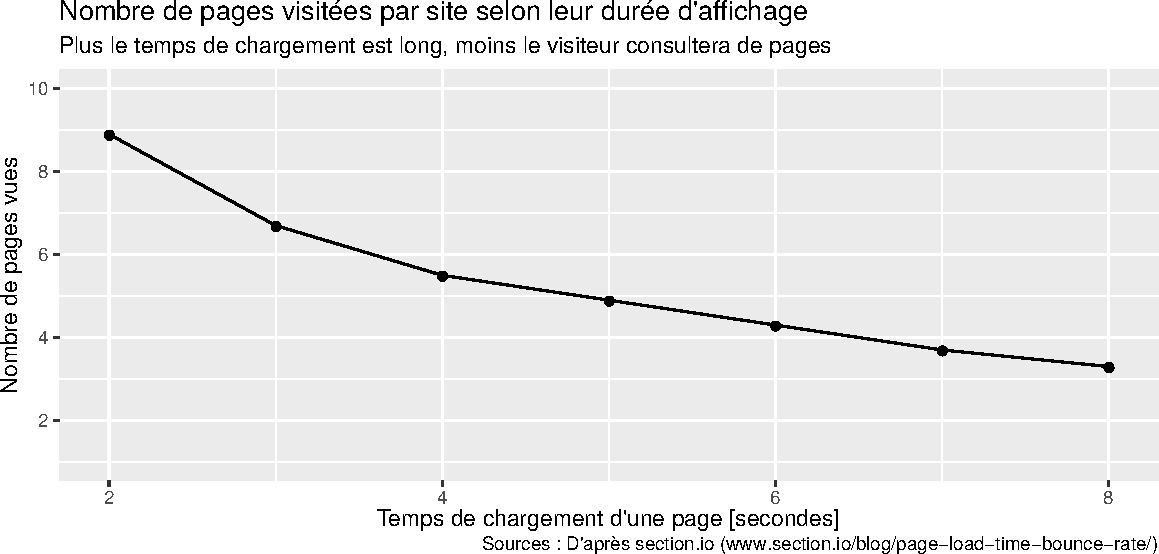
\includegraphics[width=.9\linewidth]{img/abandon_pages.pdf}
	\caption{Impact du temps de chargement d'un site web sur sa consultation. D'après \textcite{elliott_how_2017}.}
	\label{fig:page-abandon}
\end{figure}

Cet exemple est plus directement comparables aux contraintes de SimEDB.
Chaque consultation d'un indicateur de sortie correspond ainsi à la vue d'une page dans cet exemple.
Ces chiffres renforcent l'importance à accorder au temps de chargement des indicateurs, et donc à la durée de l'exécution des requêtes qui les génèrent.
Quelques secondes de différence dans le chargement suffisent ainsi à réduire drastiquement le nombre d'indicateurs que l'utilisateur acceptera d'analyser.

On peut toutefois pondérer ces comparaisons et minimiser l'importance d'écarts de l'ordre de grandeur de la seconde.
Dans le cas de SimEDB, contrairement à celui d'un site web ou d'un moteur de recherche, l'utilisateur est \og captif\fg{}.
Cela signifie qu'un thématicien souhaitant explorer les résultats produits par SimFeodal n'aura d'autre choix que de passer par SimEDB.
De même, sachant que la plate-forme présente pour lui un intérêt professionnel, le thématicien sera bien plus patient que face à un quelconque site de courses en lignes.

Dans le cadre d'environnements de type \textit{visual analysis}, il a été montré que les utilisateurs d'environnement d'exploration étaient toutefois fortement affectés par l'accroissement de délais.
Zhicheng Liu et Jeffrey Heer \autocite{liu_effects_2014} montrent ainsi qu'en introduisant une latence supplémentaire de 500 ms dans une application interactive d'exploration de données spatio-temporelles, le nombre d'interactions chute fortement, quand bien certains utilisateurs de cette application ne remarquent même pas la différence de délai.

\paragraph{Choisir un SGBD adapté à SimEDB} L'ensemble de filtres successifs a permis de réduire progressivement la quantité de solutions logicielles appropriées à l'organisation et à l'interrogation des données issues de SimFeodal.
Depuis les centaines de solutions disponibles, on parvient ainsi dans un premier temps à isoler les grands types de SGBD correspondant aux besoins identifier : les SGBD relationnels, basés sur une interrogation standardisée en SQL.
Ces outils sont ensuite départagés au prisme de leur robustesse, intrinsèque (stabilité) et sur la base de leur niveau d'adoption (pérennité).
Un \textit{benchmark} finit de restreindre la liste des possibles à quelques solutions envisageables en fonction des besoins soulevés par SimEDB.

Au regard des performances de chacun des SGBD, MapD \autocite{root_mapd_2016} présente l'avantage indéniable de la vitesse de traitement des requêtes, tout en étant compatible avec les standards de l'interrogation de données (langage de requête SQL, interfaçable via \textsf{JDBC}).
Même exécuté sur un infrastructure informatique n'est pas optimisée pour cette solution\footnote{
	MapD est ainsi un SGBD optimisé pour l'analyse sur processeurs graphiques (les GPU), présents dans les cartes graphiques modernes, contrairement aux SGBD classiques qui s'appuient sur les processeurs (CPU) pour effectuer leurs calculs.
	Dans le cadre de cette thèse, nous n'avions pas accès à un serveur doté de GPU, et MapD est donc installé sur une infrastructure à base de CPU, bien moins performante.
}, MapD est incontestablement plus performant que les autres SGBD.

On notera toutefois que le SGBD MonetDB \autocite{vermeij_monetdb_2008}, dans son implémentation intégrée MonetDBLite \autocite{raasveldt_monetdblite_2018}, affiche aussi des performances très compétitives, et aurait pu être choisi pour SimEDB, présentant notamment l'avantage d'être plus utilisé et ancien\footnote{
	Dans les faits, MonetDBLite a été le SGBD utilisé pendant une large partie de la conception de SimEDB.
	Il s'est toutefois révélé assez instable dans notre cas, faisant preuves à plusieurs reprises de corruptions de données ayant entraîné l'obligation de recréer entièrement les bases de données depuis les fichiers bruts produits par SimFeodal.
}.
Un des ouvrages de référence en \textit{visual analytics} s'interrogeait d'ailleurs sur les nouvelles possibilités et l'adéquation offertes par ce SGBD (\cite[105]{fekete_infrastructure_2010} in \cite{keim_mastering_2010}).

Nous avons au final préféré MapD, en particulier parce que les données issues de SimFeodal sont amenées à augmenter, renforçant donc petit à petit l'écart de performance entre MapD et MonetDB.
Par ailleurs, par une heureuse coïncidence, MapD a été placé sous licence libre peu avant que nous n'ayons à nous pencher réellement sur les problèmes de performances et de robustesse qui apparaissaient suite à l'augmentation du nombre de simulations effectuées.


\subsection{Structuration des données de SimFeodal}

Le choix d'un SGBD est une étape indispensable à la mise en place d'une base de données, mais il ne concerne que le domaine technique, voire méthodologique, mais aucunement le domaine conceptuel.
Un SGBD est un support logiciel qui permet le stockage et l'organisation de données.
Il n'est utile qu'une fois que le mode d'organisation des données a été décidé.
L'organisation a proprement parler des données est explicitée dans un modèle conceptuel, nommé Modèle Conceptuel de Données (MCD).
Un MCD est propre à un ensemble de données d'une part\footnote{
	Le MCD décrit la manière dont les données sont stockées, organisées et mises en relations.
	Il ne peut donc être générique, et doit être modifié quand la structure des données évolue.
}, et un ensemble de problématiques d'autres part\footnote{
	Il y a une infinité de possibilité d'organisation d'un même jeu de données.
	Le MCD permet d'organiser ces données en vue de répondre à des questions, exprimées sous formes de requêtes particulières.
	Appliquées au même jeu de données, différents MCD permettront de répondre plus ou moins facilement (et de manière plus ou moins performante) à certaines questions.
}.
Ce MCD décrit donc les \og tables\fg{}, leur composition (attributs) et les liens entre tables qui permettent de mener des interrogations croisées.
Par exemple, on peut avoir une table élèves, contenant les informations relatives aux élèves d'un établissement, une table enseignants, et une table classe qui permet de faire le lien entre les élèves d'un enseignant, ou au contraire entre un élève et tous ses enseignants.

Les choix de conception d'un MCD sont fortement lié aux types de SGBD dans lesquelles ils doivent être implémentés.
On ne peut que difficilement implémenter un MCD très relationnel dans un SGBD pensé collection (NoSQL par exemple).
À l'inverse, le stockage d'informations très hétérogènes sur un ensemble d'individus sera complexe à implémenter au sein d'un SGBD relationnel.

Pour décider de la manière la plus efficace d'implémenter les données issues de SimFeodal dans un SGBD, et donc du MCD à suivre, il convient de revenir aux spécificités des données produites par le modèle d'une part, et d'autre part de réfléchir aux modes d'interrogations privilégiés, lesquels orienteront la conception du MCD.


\paragraph*{Pré-traitement des données}
Les données produites par un modèle de simulation sont des données \og brutes\fg{}, c'est-à-dire qu'elles ne sont pas organisées de manière rationnelle, contiennent une quantité non négligeable d'informations incomplètes, superflues ou erronées.
\begin{itemize}
	\item Par exemple, quand une simulation est arrêtée en cours, soit volontairement, soit en raison d'un \textit{bug}, les données générées par le modèle sont \textbf{incomplètes} : elles ne concernent qu'une partie des pas de temps attendus.
	Elles sont pourtant exportées dans les fichiers bruts, rendant ceux-ci hétérogènes en matière de complétion des informations enregistrées.
	Pour pouvoir analyser une expérience, il faudra supprimer ces données incomplètes pour qu'elles n'influence pas l'étude des simulations complétées et donc comparables.
	\item De la même manière, il arrive qu'on exécute, par erreur, plusieurs fois les mêmes simulations.
	Dans ce cas, le nombre de réplications de chacune des expériences ne sera pas systématiquement le même.
	Cela pose un problème de comparabilité dû à tailles d'échantillonnage différentes.
	On fait donc face à un problème de données \textbf{superflues} : il faudra supprimer une partie de ces simulations des données avant de pouvoir les traiter.
	\item On peut enfin voir subvenir des erreurs d'exécution du modèle au niveau des agents, par exemple quand, en raison d'un \textit{bug}, un agent en interroge un autre qui a disparu depuis.
	Il arrive ainsi fréquemment que des foyers paysans déclarent une appartenance à un agrégat qui a disparu depuis, faute à une mise à jour échouée dans le modèle.
	Dans ces cas, les données seront aussi inscrites dans les sorties de SimFeodal, quand bien même elles sont \textbf{erronées}.
\end{itemize}

Les données brutes doivent donc nécessairement être vérifiées, filtrées, nettoyées et retravaillées avant de pouvoir les exploiter en vue de générer les indicateurs de sortie.

\paragraph*{Organisation des données}
Même pré-traitées, les données brutes conservent une structure tabulaire assez peu adaptées à un traitement.
les attributs de chacun des types d'agent sont enregistré dans des fichier spécifiques.
Que ces fichiers aient été nettoyés ou non, ils demeurent fondamentalement isolés les uns des autres.
Une partie des indicateurs repose sur des analyses croisant différents types d'agents (dans quels pôles les agrégats s'inscrivent-ils par exemple ?), et il est donc nécessaire de permettre -- et de fluidifier -- ces requêtes croisées.
On a mentionné le choix de SGBD relationnels, il convient donc de concevoir et d'implémenter, dans le SGBD choisi, les relations entre les différentes tables individuelles qui proviennent des sorties brutes d'un modèle.



\subsubsection{Quel modèle de données ?}

Les MCD sont propres à chaque ensemble de données et questionnement associés.
Il y a toutefois des grandes tendances dans l'organisation des données.
Le MCD peut ainsi être catégorisé, selon sa forme, dans des familles de modèles de données.
On nomme ces catégories \og modèles logiques\fg{} ou \og schémas\fg{} (\textit{logical schema} en anglais).
Ceux-ci décrivent la manière dont les données sont structurées et surtout reliées les unes aux autres, d'une manière générique contrairement aux MCD.

\paragraph*{Un modèle \og en étoile\fg{}}

Les bases de données relationnelles peuvent s'appuyer sur de nombreux schémas différents.
Sans entrer dans le détail, notons que chacun des schémas existant présente des avantages et des inconvénients liés aux types de requêtes qui lui seront adressés.
Par exemple, un schéma \og en étoile\fg{} \autocite{noauthor_star_2018} privilégie l'efficacité de requêtes d'agrégations et de jointures, au détriment de la robustesse des données et de la \og liberté\fg{} des requêtes.
Certains types de requêtes, complexes, seront ainsi difficiles, voire impossibles, à exprimer dans ce type de schéma.

Au contraire, un schéma \og en flocons\fg{} \autocite{noauthor_snowflake_2018} peut se révéler plus permissif en terme de capacités de requêtes.
L'inconvénient est une plus forte complexité des requêtes de bases (exprimées de manière plus verbeuses et tortueuses) et donc d'une expressivité moindre.

Pour choisir un schéma, et donc une manière d'organiser la base de données, il convient donc de savoir -- ou de prévoir -- le type de requêtes qui lui seront adressées.
Dans le cas des données de SimFeodal, les indicateurs avaient été définis avant que le besoin d'une interrogation performante et structurée n'apparaisse.
On connaissait déjà les indicateurs nécessaires et le type de requêtes associés.
Nous savions ainsi qu'une majorité des requêtes seraient des tâches d'agrégations simples (nombre d'agrégats au cours du temps, taux de foyers paysans dispersés au cours du temps etc.), pour lesquelles il fallait minimiser la complexité des requêtes et calculs.

Il a été choisi de partir d'un schéma en étoile, puisque celui-ci se montre extrêmement efficace pour réduire les besoins en jointures -- chronophages -- et pour des tâches d'agrégations lourdes.

\clearpage
\begin{figure}[H]
	\centering
	\captionsetup{width=\linewidth}
	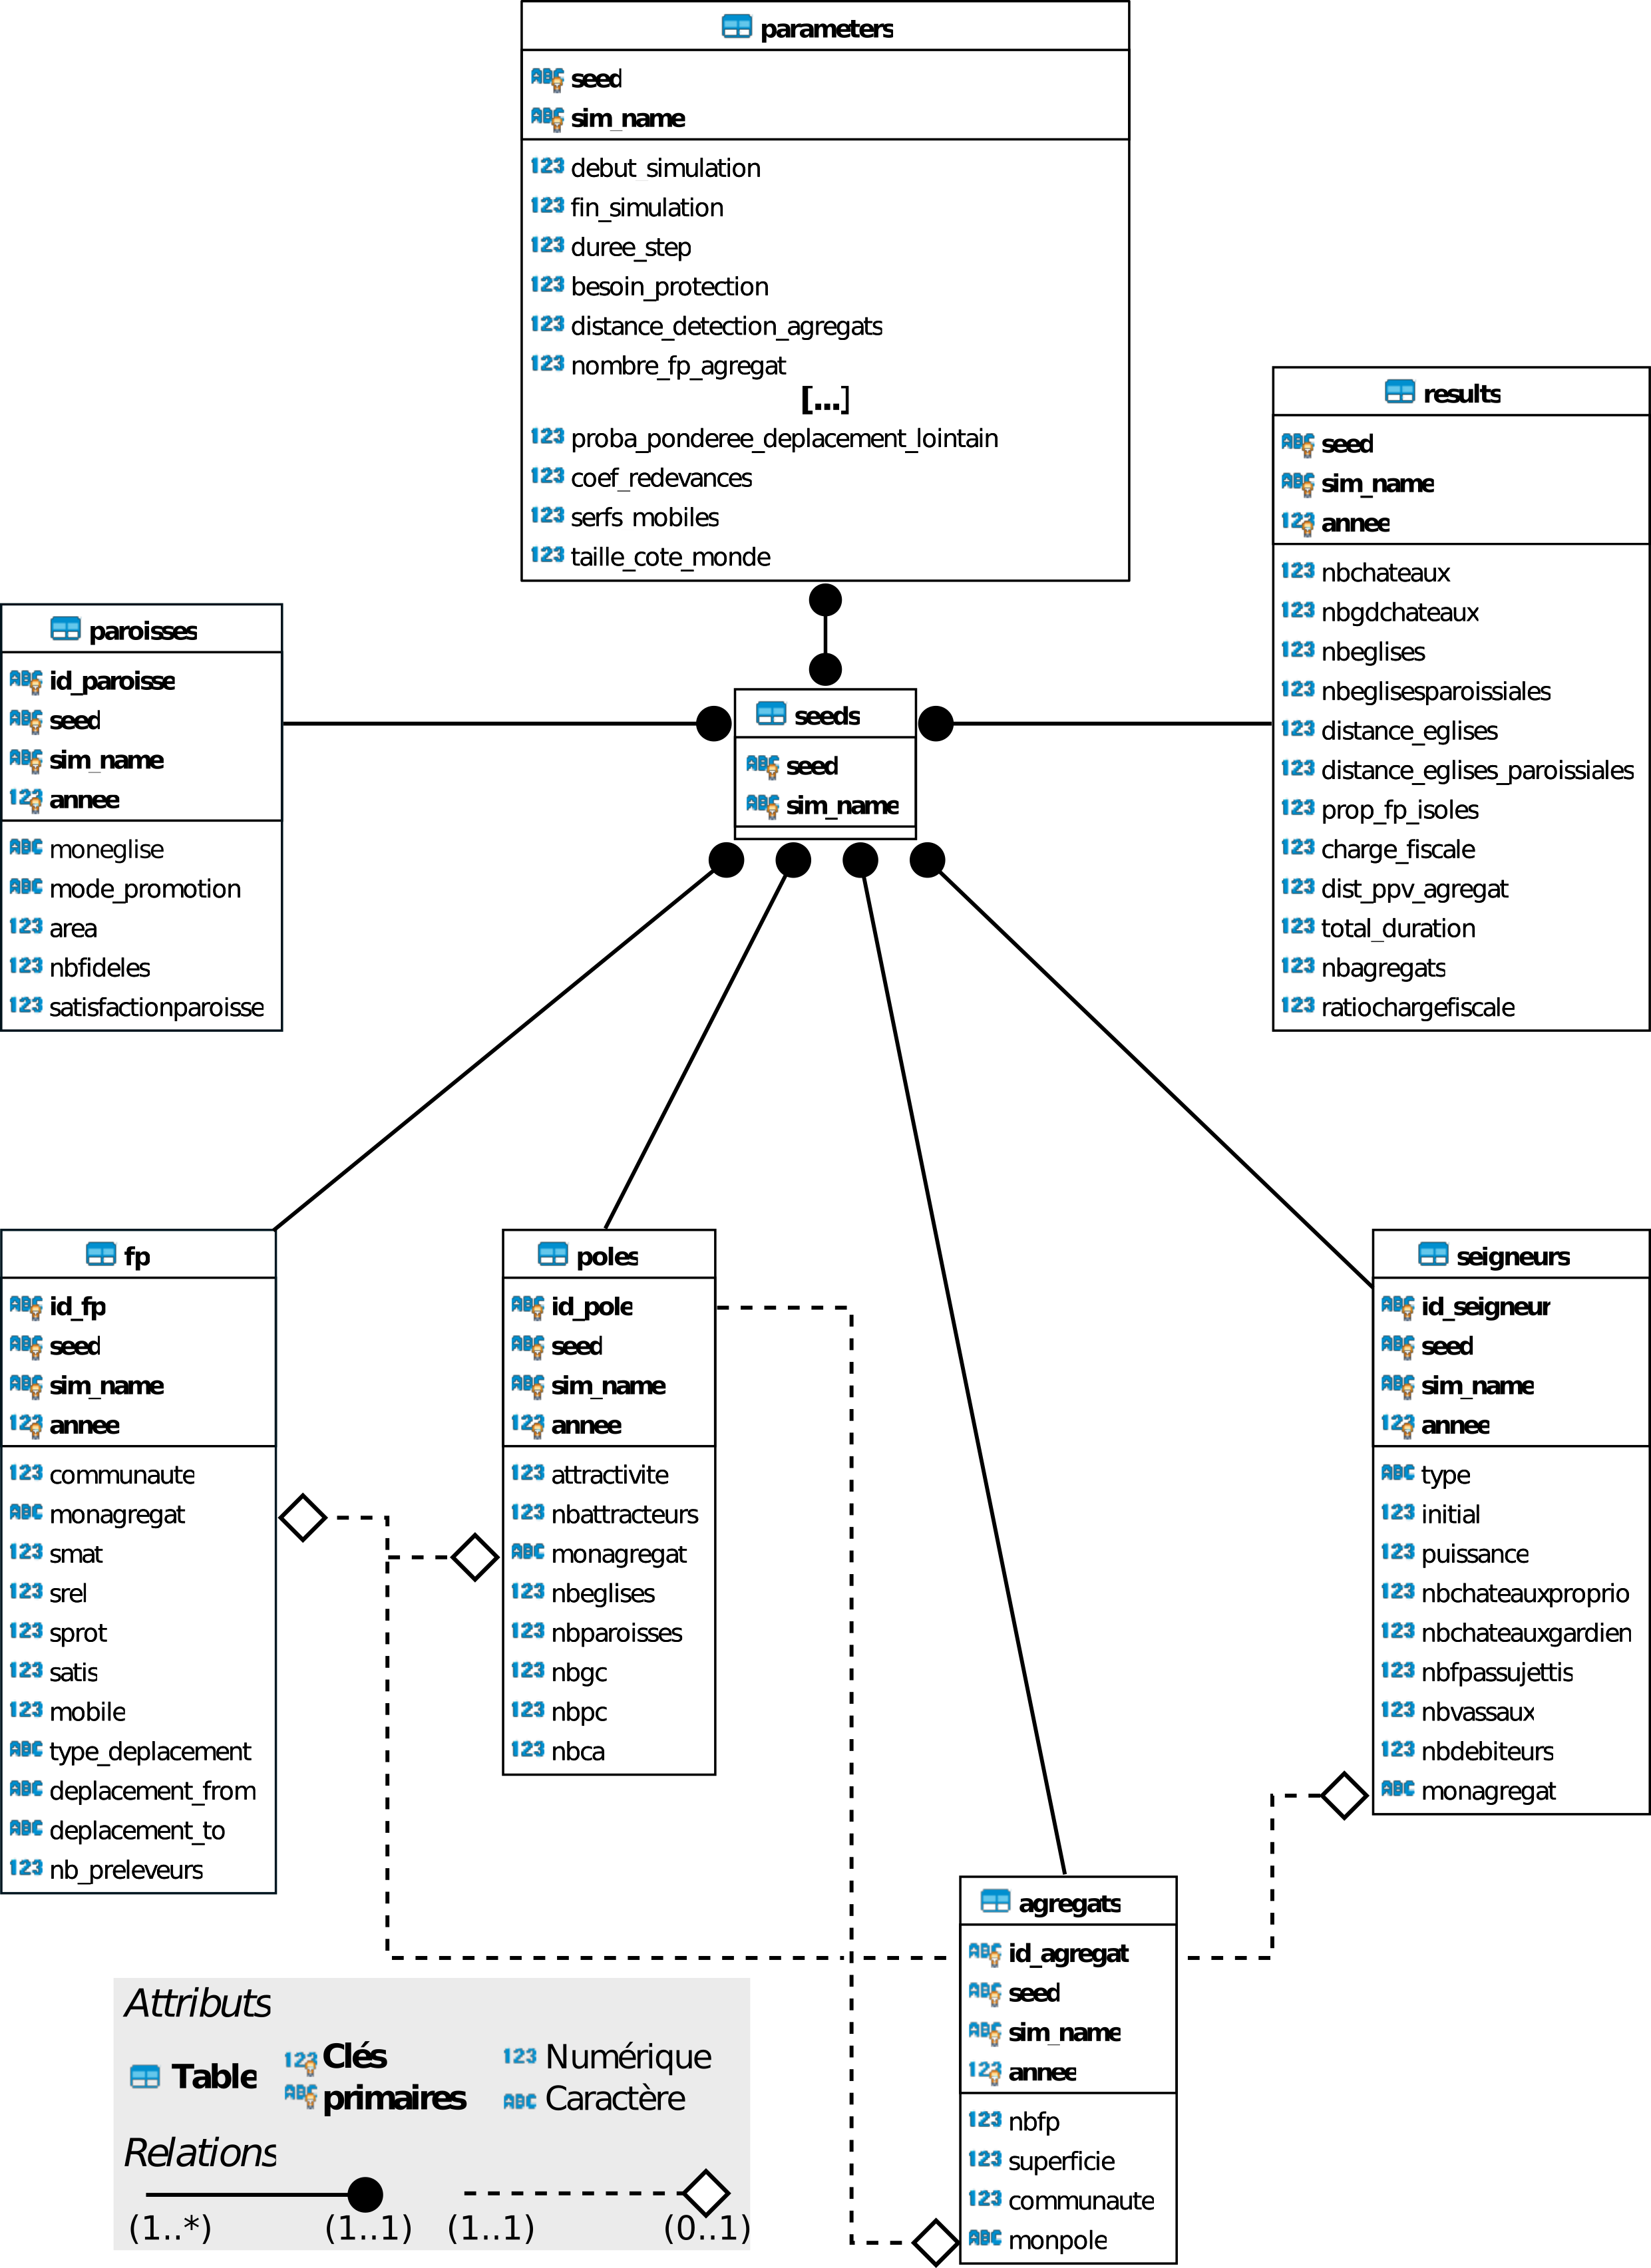
\includegraphics[width=\linewidth]{img/MCD_SimEDB_repris.png}
	\caption{Modèle Conceptuel de Données (MCD) des données en sortie de simulation de SimFeodal telles qu'implémentées dans SimEDB.}
	\label{fig:MCD_SimEDB}
\end{figure}

Au centre de cette étoile (voir \cref{fig:MCD_SimEDB}), il était donc évident de disposer une table simple, contenant les informations sur lesquelles une majorité des agrégations seraient effectuées : les simulations, identifiées par leur nom (\texttt{sim\_name}, qui permet de savoir de quelle expérience ces simulations dépendent) et leur identifiant unique, la graine aléatoire utilisée (\texttt{seed})\footnote{
	La graine aléatoire ne constitue en tant que tel pas un identifiant unique : comme son nom l'indique, elle est aléatoire et présente donc un risque de répétition.
	Dans Gama, cette graine aléatoire est une valeur qui varie de 0 à 1 et est composé de 19 décimales.
	Il y a donc potentiellement $10^{19}$ graines aléatoires uniques, ce qui est en soi une quasi garantie d'unicité.
	Notons de plus que dans le MCD de SimEDB, la graine aléatoire est systématiquement associée au nom de l'expérience.
	Même en menant un million de réplications, la probabilité que deux simulations partagent la même graine aléatoire serait largement inférieure à 1\%.
	La graine aléatoire constitue donc un identifiant unique robuste dans notre cas.
}.

\paragraph*{Relier les tables}

Toutes les tables contenant les enregistrements individuels des agents (\texttt{fp} pour les foyers paysans, \texttt{paroisses} pour les églises paroissiales, etc.) sont donc liées directement à cette table centrale (intitulée \texttt{seeds} ici).

En dehors de ces tables liées aux agents, deux autres tables \og globales\fg{} sont présentes : une table \og \texttt{results}\fg{}, qui contient des informations agrégées sur l'état de chaque simulation à chaque pas de temps.
Ces informations, par exemple le taux de foyers paysans isolés (champ \og \texttt{prop\_fp\_isoles}\fg{}), sont redondantes : elles pourraient être calculées directement depuis la table renseignant les foyers paysans, en faisant un ratio entre le nombre de foyers paysans sans agrégat et leur nombre total.
Pourtant, pour des raisons d'efficacité autant que de clarté, il a été choisi de dupliquer, en les pré-calculant, ces informations qui sont interrogées extrêmement souvent pour calculer les indicateurs de SimFeodal.

Autre table ne répondant pas au schéma classique, la table \og \texttt{parameters}\fg{} fournit toutes les méta-données sur les simulations.
 On y retrouve par exemple les valeurs de paramètres de chacune des simulations, identifiées toujours par le couple \texttt{sim\_name} et \texttt{seed}.
Cette table est la seule à être reliée de manière bi-directionnelle à la table centrale (\texttt{seeds}), en particulier en raison de l'usage qui en est fait interactivement (voir l'\cref{enc:usage-MCD-SimEDB}).

Notons tout de même que l'on s'éloigne légèrement du classique schéma en étoile en raison des relations que nous avons choisi d'insérer entre les tables des différents agents (relations notées en pointillées dans la \cref{fig:MCD_SimEDB}).
Intégrer ces relations dans la table centrale aurait considérablement complexifié cette dernière, mais pour autant, elles étaient nécessaires : SimFeodal est un modèle complexe, dans lequel des interactions sont présentes à plusieurs niveaux entre différents types d'agents.
La base de données résultant de ce modèle complexe l'est donc nécessairement aussi : on doit implémenter, dans la base de données, des relations entre les  tables pour chacune des interactions entre les agents du modèle.
Ici, ces relations permettent par exemple d'étudier la composition des pôles autour de chaque agrégat, et ainsi d'étudier le lien entre poids du pôle (en nombre d'attracteurs) et poids de l'agrégat (en nombre de foyers paysans).

Ces indicateurs, situés à l'intersection de différents types d'agents, sont toutefois moins utilisé que les indicateurs plus directs (\hl{ref à chapitre 3, indicateurs}).
Les requêtes correspondantes, moins fréquentes, ne perturbent pas les logiques et performances d'ensemble de SimEDB : elles auraient plus facilement exprimées dans un schéma \og en flocons\fg{}, mais leur relative rareté ne remet aucunement en cause l'organisation générale du MCD.


\subsubsection{Un modèle de données pour favoriser l'interrogation et le filtrage conjoint}

Le schéma choisi et le Modèle Conceptuel de Données (MCD) associé, permettent  une interrogation rapide des données en simplifiant les tâches d'agrégation et en minimisant la quantité de jointures nécessaires à la génération des indicateurs de sortie.
Le choix de s'écarter légèrement du schéma en étoile présente un autre avantage, extrêmement utile, dans le cadre d'une exploration interactive des indicateurs de SimFeodal.
En effet, comme on l'a vu auparavant (\cref{subsec:explorer-simedb}), dans SimEDB, on compare les simulations en les isolant à partir des valeurs de paramètres qui leur correspondent, via un acte de \textit{brushing} des valeurs de paramètres présentées dans un graphique en coordonnées parallèles interactif.
Du côté du MCD, la table correspondante est la table \texttt{parameters}.
Quand l'utilisateur sélectionne un sous-ensemble de valeurs de paramètres, la table est filtrée, et ne renvoie donc que les simulations correspondantes.

C'est ici que l'intérêt de la table \texttt{seeds} et de son lien bidirectionnel avec la table \texttt{parameters} apparaît : une fois \texttt{parameters} filtrée, cette sélection est renvoyée à la table \texttt{seeds}, et se répercute donc directement à toutes les autres tables.
Avec une unique requête, qui plus est sur une table de faible dimension (\texttt{seeds} ne comporte que deux champs), le filtrage est donc extrêmement véloce, accélérant d'autant le filtrage des autres tables et donc la génération des indicateurs de sortie.
Ces étapes de filtrage successifs, optimisées par l'architecture choisie pour les données de SimFeodal, sont présenté dans l'\cref{enc:usage-MCD-SimEDB}.

\clearpage

\begin{encadre}{Un exemple d'interrogation de la base de données de SimEDB.}{usage-MCD-SimEDB}
	
	La \cref{fig:MCD_SimEDB_etapes} présente l'ensemble des étapes qui permettent de générer un indicateur de sortie.
	Cette planche montre un exemple de sélection faite dans l'application SimEDB, et décrit la manière dont cette sélection est répercutée à travers le MCD de SimFeodal (\cref{fig:MCD_SimEDB}).
	La démarche aboutit par la sélection d'un ensemble de données, qui répondent à un critère sur deux paramètres du modèle.
	Cette sélection est ensuite utilisée pour générer un indicateur de sortie, ici, l'évolution du nombre d'agrégats au cours du temps.

\begin{figure}[H]
	\centering
	\captionsetup{width=\linewidth}
	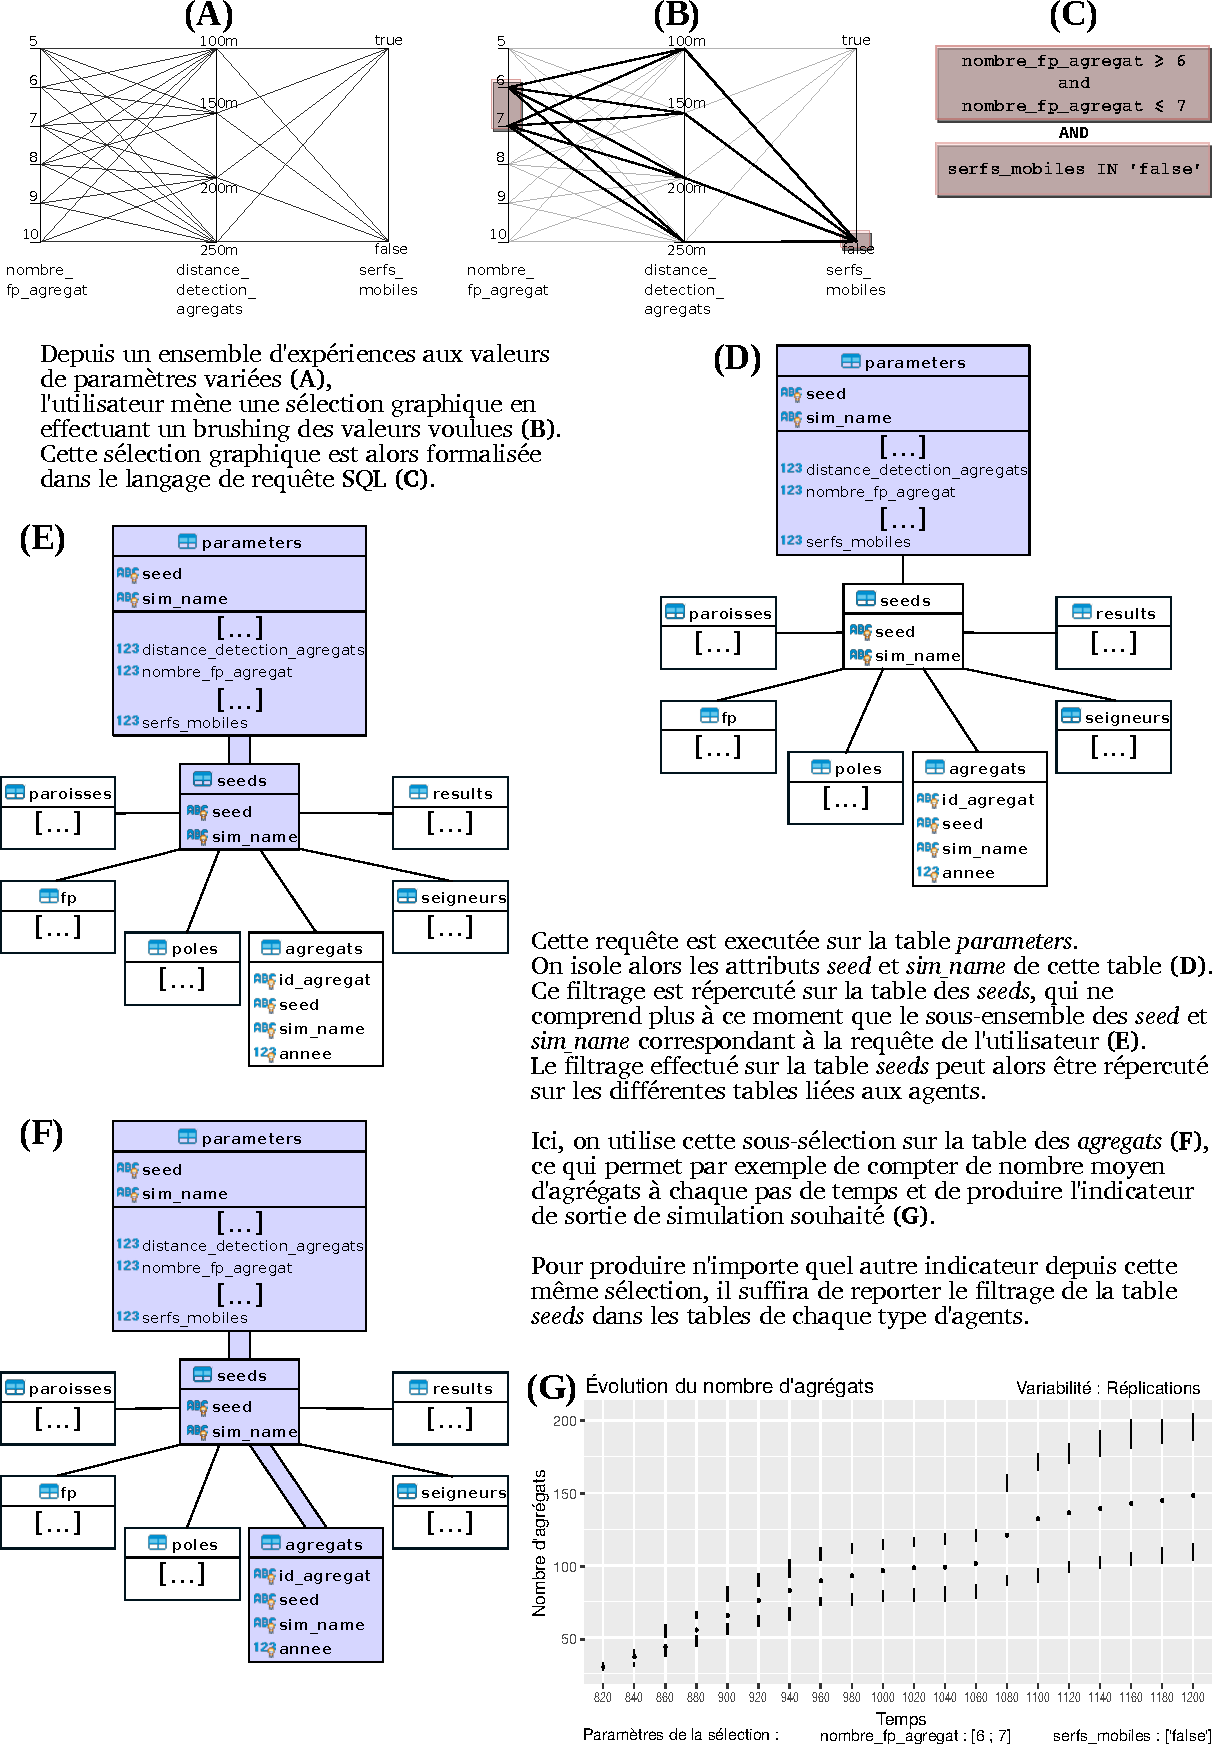
\includegraphics[width=\linewidth]{img/MCD_exemple_requetes.pdf}
	\caption{De la sélection interactive à l'indicateur de sortie.}
	\label{fig:MCD_SimEDB_etapes}
\end{figure}
\smallskip
\end{encadre}

\subsection*{Une organisation dédiée à l'exploration interactive}
La présentation des choix d'organisation de données témoigne d'une visée résolument applicative, c'est-à-dire visant à penser l'organisation, la structuration et les SGBD d'implémentation, comme au service de la plate-forme d'exploration SimEDB.
Le SGBD choisi, MapD, est ainsi un logiciel particulièrement adapté aux besoins identifiés, c'est-à-dire à une efficacité et une robustesse d'interrogation des données générées par SimFeodal.
MapD est interrogeable de manière universelle, via des protocoles de connexion standards, au moyen d'un langage qui fait office de \textit{lingua franca} de l'interrogation de données, le SQL.
Au sein du SGBD, la structure des données, révélée dans le MCD qui adopte une structure \og en étoile\fg{}, vise aussi à faciliter et à optimiser la vitesse des requêtes visant à générer les indicateurs de sortie de SimFeodal.
Cette structure de données est enfin pensée, en amont, pour minimiser le nombre de requêtes nécessaires à l'affichage des indicateurs, dans un cadre interactif, correspondant à des sous-ensembles des nombreuses simulations effectuées au cours de la construction, du paramétrage et de la calibration de SimFeodal.

Il est important de noter qu'en l'absence de ces choix de conception de base de données, de la modélisation conceptuelle jusqu'à l'implémentation technique, la plate-forme d'exploration des données SimEDB, que nous allons maintenant présenter plus en détail, n'aurait pu être conçue, élaborée et bâtie de manière convaincante.

%\setcounter{section}{3}
%\clearpage
\section[Une plate-forme d'exploration de données de simulations : SimEDB]{Une plate-forme d'exploration de données de simulations : SimEDB%
\sectionmark{SimEDB}}\label{sec:SimEDB}

La \cref{sec:explorer-sorties-simfeodal} (\cnameref{sec:explorer-sorties-simfeodal}) a décrit les étapes successives d'avancement dans l'exploration des données en sortie de SimFeodal, depuis l'observation en direct des simulations (\og pré-filtrage\fg{}) jusqu'au besoin d'une plate-forme permettant l'exploration et la comparaison interactive des sorties de simulation.
La plate-forme proposée en réponse à ce besoin, SimEDB\footnote{
\textbf{Sim}Feodal \textbf{E}xploration \textbf{D}ash\textbf{B}oard, voir la note de bas de page \ref{ftn:origine-simedb}, \cpageref{par:introduction-nom-simedb}.
}, dans un objectif de généricité et d'adéquation, se devait aussi de répondre à de nombreuses contraintes, aussi bien liées aux possibilités offertes qu'à l'usage qui en serait fait.
Dans cette partie, nous nous attacherons donc à présenter les contraintes qui ont guidé la conception de SimEDB, ainsi que les choix, méthodologiques et techniques, qui en ont résulté.\vspace{-0.5cm}

\subsection{Contraintes}

\subsubsection{Adapter la complexité aux utilisateurs}

Dans le domaine de l'Interface Homme-Machine (IHM), il est courant de considérer qu'un outil d'analyse et de représentation doit être adapté à un public.
La \cref{fig:cartography3}, emblématique de la conception de géovisualisations par Alan \textsc{MacEachren}, replace ainsi les types d'usage d'une plate-forme d'exploration selon trois axes : le niveau d'expertise des utilisateurs visés (\textit{users}), le niveau d'interaction souhaité (\textit{interaction}) et l'objectif poursuivi par la (géo)visu\-alisation (\textit{task}).
D'après l'auteur, à un niveau d'expertise de l'utilisateur correspond un unique degré d'interaction et un unique objectif : dans le cube, seule une \og droite\fg{} des usages possibles est présente.
L'auteur décompose ces usages en quatre types :
\begin{itemize}
	\item Pour le grand public (\textit{users} de type \textit{public}), l'objectif est de transmettre une information simple (\textit{info sharing}). Le niveau d'interaction avec la géovisualisation doit donc être faible. Il s'agit d'une tâche de présentation (\textit{present}).
	\item Pour un public légèrement plus connaisseur, on peut augmenter le niveau d'interaction. On entre alors dans un but de synthèse (\textit{synthesize}).
	\item En ciblant un niveau encore supérieur d'expertise chez l'utilisateur, et en visant à de la construction de connaissance plus qu'à une transmission de connaissance, on augmente encore le niveau d'interaction.
	La géovisualisation a alors pour but l'analyse (\textit{analyze}).
	\item Au plus haut niveau d'interaction, d'expertise et de recherche, la géovisualisation peut servir d'outil d'exploration (\textit{explore}).
\end{itemize}

%\begin{figure}[H]
%\hspace*{\fill}%
%\begin{minipage}[t]{.46\linewidth}
%\centering
%\captionsetup{width=.9\linewidth}
%\vspace{0pt}
%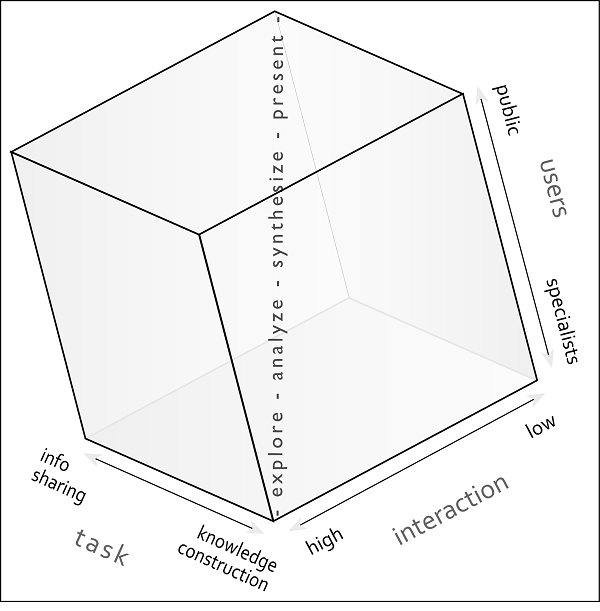
\includegraphics[width=\linewidth]{img/CV35-Fig2a-600.png}
%\caption{\og \textit{An update to Cartography³, 10 years after its conception}\fg{}, par \cite{coltekin_geovisualization_2018}, d'après \cite[10]{maceachren_geovisualization_2004}.}
%\label{fig:cartography3}
%\end{minipage} \hfill
%\begin{minipage}[t]{.46\linewidth}
%\centering
%\captionsetup{width=.9\linewidth}
%\vspace{0pt}
%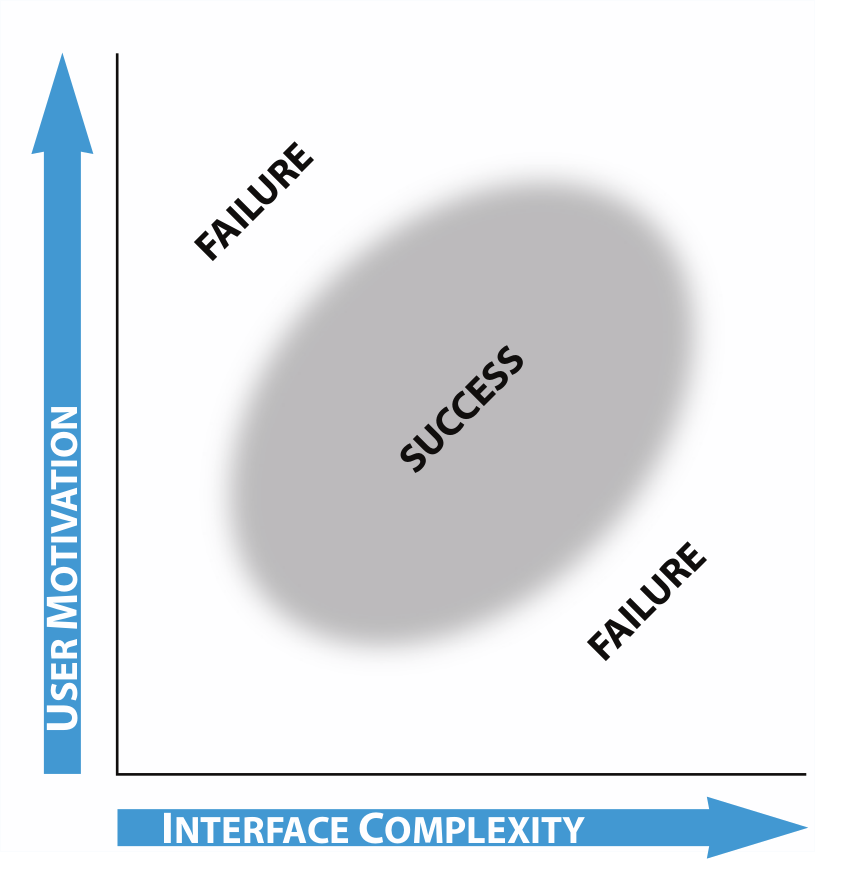
\includegraphics[width=\linewidth]{img/Roth_Interface_Complexity.png}
%\caption{\og \textit{Interface complexity versus user motivation. }\fg{}, \cite[79]{roth_interactive_2013}.}
%\label{fig:interface-complexity}
%\end{minipage}
%\medskip
%\end{figure}

\begin{figure}[H]
\centering
\vspace{0pt}
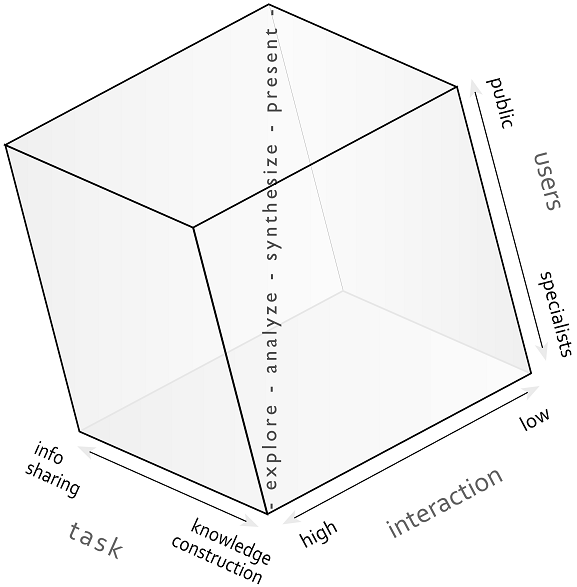
\includegraphics[width=.7\linewidth]{img/cartography3.png}
\captionsetup{width=.7\linewidth}
\caption{\og \textit{An update to Cartography³, 10 years after its conception}\fg{}, par \cite{coltekin_geovisualization_2018}, d'après \cite[10]{maceachren_geovisualization_2004}.}
\label{fig:cartography3}
\end{figure}

\textcite[16]{roth_interactivity_2015} commente cette figure en effectuant une assimilation entre niveau d'interaction et complexité de l'interface de l'outil de géovisualisation : \og All participants agreed that user expertise requires increased interface complexity, as suggested by the Cartography³ framework\fg{}.

La plateforme SimEDB est conçue pour être utilisée par des experts thématiques (l'équipe de modélisation de SimFeodal), avec un objectif clairement inscrit dans la construction de connaissance.
A ce titre, et d'après \textsc{MacEachren}, le niveau d'interaction avec l'outil de géovisualisation devrait être élevé (forte complexité de l'interface pour \textsc{Roth}) et ancrer l'usage dans une dimension exploratoire.



\paragraph*{Des utilisateurs hétérogènes mais captifs}

SimEDB est pourtant pensé à un niveau intermédiaire, entre l'analyse et la synthèse, dans le cube de la \cref{fig:cartography3}.
Il ne s'agit ainsi pas d'explorer des données, au sens de MacEachren, qui sous-entend par cette exploration (\textit{explore}) la recherche d'informations dans un jeu de données inconnu de l'utilisateur.
Le besoin identifié consiste à permettre aux utilisateurs d'explorer des sorties de simulation à travers des indicateurs déjà pensés et constitués.
Il ne s'agit pas de proposer un outil d'exploration de données brutes, permettant de créer à la volée des nouveaux indicateurs, via une approche d'exploration \og naïve\fg{}.
Au contraire, l'exploration est guidée par les indicateurs, et la tâche s'apparente plus à de l'analyse de résultats de simulations, voire à de la synthèse des spécificités des résultats issus d'expériences différentes.
L'objectif de SimEDB s'écarte donc du \og modèle\fg{} de \textsc{MacEachren}, puisqu'il ne se situe pas sur la \og droite\fg{} des usages (voir la \cref{fig:cartography3-simedb}).

\begin{figure}[H]
\hspace*{\fill}%
\begin{minipage}[t]{.46\linewidth}
\centering
\captionsetup{width=.9\linewidth}
\vspace{0pt}
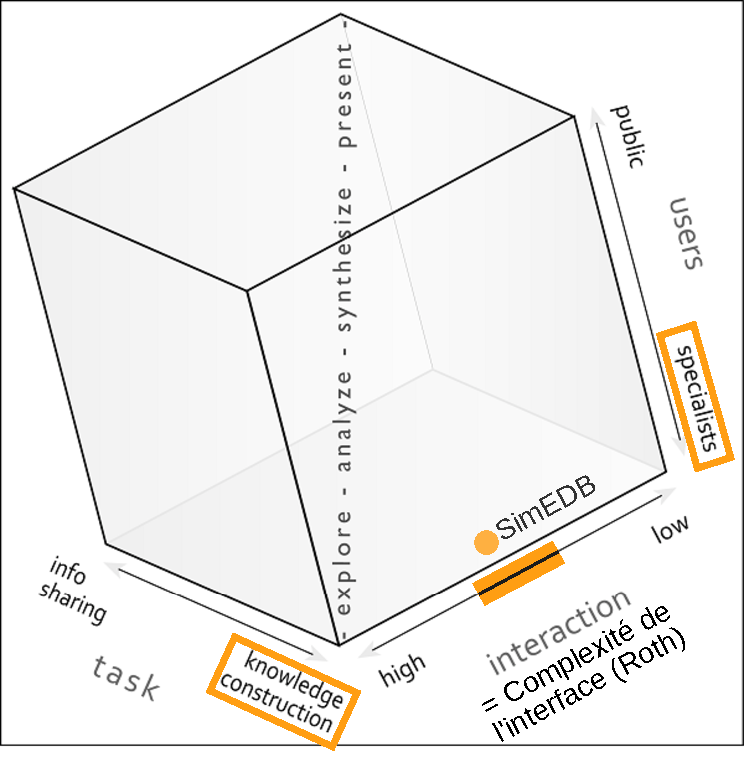
\includegraphics[width=\linewidth]{img/Cartography3_SimEDB.pdf}
\caption{Positionnement de SimEDB dans le cube \textit{Cartography³} de \textsc{MacEachren}.}
\label{fig:cartography3-simedb}
\end{minipage} \hfill
\begin{minipage}[t]{.46\linewidth}
\centering
\captionsetup{width=.9\linewidth}
\vspace{0pt}
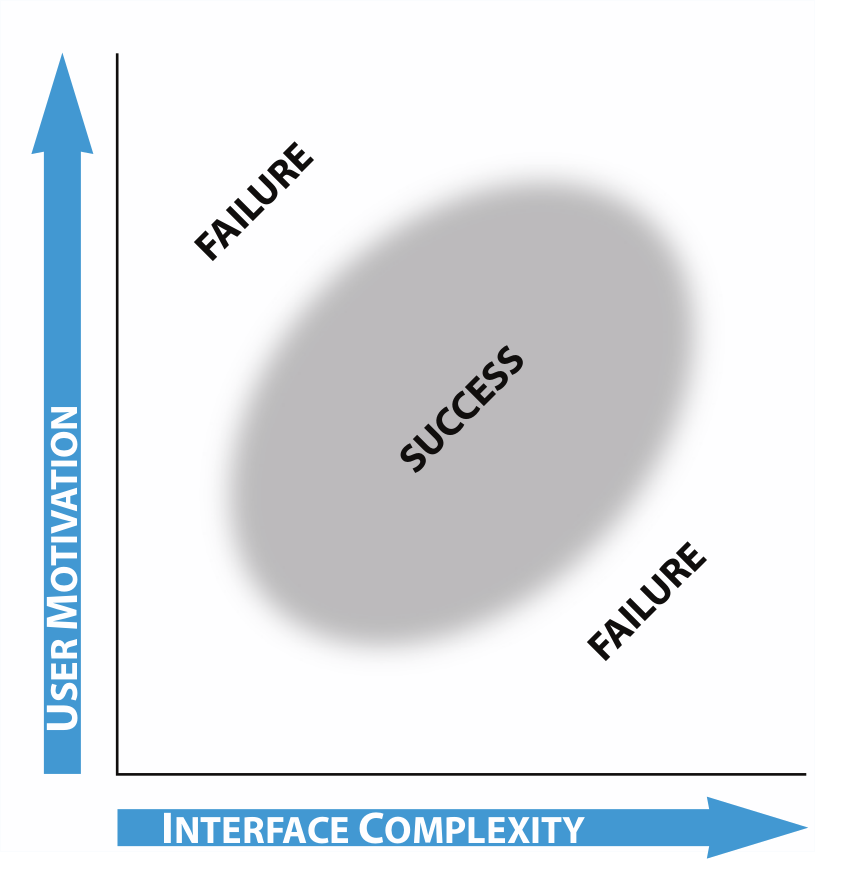
\includegraphics[width=\linewidth]{img/Roth_Interface_Complexity.png}
\caption{\og \textit{Interface complexity versus user motivation. }\fg{}, \cite[79]{roth_interactive_2013}.}
\label{fig:interface-complexity}
\end{minipage}
\medskip
\end{figure}

Cet écart au modèle conceptuel de MacEachren s'explique notamment par la diversité des utilisateurs de SimEDB.
Il serait absurde de qualifier un niveau d'expertise général des utilisateurs tant les spécificités de cette expertise sont nombreuses.
Entre des profils de spécialiste thématiciens, de modélisateurs ou encore de géomaticiens, l'expertise est présente, mais concernant des champs différents, toutefois tous intéressés par l'exploration des sorties de SimFeodal.

Il est dès lors peu évident de se fixer sur un degré de complexité à atteindre dans la plate-forme d'exploration : un niveau faible serait frustrant pour les utilisateurs avancés, et un niveau avancé serait source de confusion et donc de perte de motivation pour les utilisateurs moins expérimentés (\cref{fig:interface-complexity}).

Une spécificité du cas d'usage de SimEDB permet toutefois de miser sur une bonne motivation générale des utilisateurs, et donc sur la possibilité de créer un outil à l'interaction plus complexe qu'un simple présentoir de données.
Contrairement à une utilisation grand public, qui ne présente aucun engagement vis-à-vis d'une interface d'exploration de données, ou à l'inverse contrairement à des domaines experts où chaque utilisateur dispose de ses propres outils et méthodes pour explorer un jeu de données, le public cible de SimEDB est \og captif\fg{}.
On entend par là que les utilisateurs concernés par SimEDB ne disposent pas d'autre solution que de passer par cette plate-forme pour explorer les données issues de sortie de simulation, en particulier en raison des contraintes liées aux caractéristiques de ces données (leur masse par exemple, voir la \cref{subsec:donnees-indicateurs}, \cnameref{subsec:donnees-indicateurs}).
On peut dès lors se permettre de développer une interface plus complexe que si l'on visait un plus large public.

\paragraph*{Intuititivé de l'usage au regard des applications traditionnelles}

En dépit de cette motivation, les utilisateurs de SimEDB demeurent majoritairement des experts thématiciens, potentiellement peu familiarisés à l'exploration de données interactives.
Afin que le temps d'exploration des données issues de SimFeodal soit dévoué à la compréhension et à la synthèse de ces données plutôt qu'à un apprentissage ou amélioration en exploration de données, il a été choisi de créer une application aussi simple que possible au regard des fonctionnalités principales qu'elle devait permettre : observer les indicateurs de sortie de simulation pour des expériences données, et les comparer entre elles aussi efficacement que possible.

Il n'était donc pas question de construire un nouveau \og logiciel expert \fg{}, doté de dizaines de fonctionnalités avancées, mais au contraire, de simplifier au maximum l'interface pour ne pas encombrer et complexifier l'utilisation de ces fonctionnalités principales.

On souhaitait une plate-forme aussi épurée que possible, plutôt que de partir, par exemple, sur la personnalisation et l'adaptation de l'un des outils d'exploration existants et dédiés à offrir une forte possibilité de manipulation\footnote{
\colorbox{Cyan}{Lena : \og Éventuellement dire pourquoi recherche de généricité dans un créneau bien spécifique ?}
}.


\subsubsection{Efficacité}

Dans la description du choix du SGBD, on a mentionné une première fois l'intérêt de disposer d'une solution d'interrogation de données qui garantisse une certaine rapidité dans l'exécution des requêtes.
Sans entrer dans le détail des recherches en IHM, on peut compléter ce besoin de rapidité par deux aspects complémentaires.
Une solution interactive qui minimise les latences permet (1) de motiver l'utilisateur, c'est-à-dire de ne pas le décourager d'utiliser l'application, et (2) de lui faire conserver sa concentration\footnote{
Avant de spécifier ce sujet, notons que quand le délai entre une interaction avec un outil informatique et le retour qu'il doit produire (affichage de graphique par exemple) est important, l'utilisateur perd en capacité d'association entre son action et le retour observé.
Typiquement, dans un processus d'exploration de données, plus ce délai est faible, plus l'utilisateur peut mobiliser son intuition pour évaluer, par exemple, les relations entre des variables ou des individus.
} (\textit{focus}).

Le premier point a été abordé plus haut (\cref{subsubsec:interroger-robuste-efficace}), et surtout, en raison de la \og captivité\fg{} de l'utilisateur évoquée ci-dessus, ne s'applique que marginalement à notre cas d'étude.
Des délais trop importants pourraient décourager l'utilisateur, mais en l'absence d'alternative pour explorer les sorties de simulation, cela n'a pas un impact trop important.

\paragraph*{Conserver la concentration}

Le problème de la concentration de l'utilisateur demeure, lui, critique.
Des études ont montré, depuis longtemps \autocite{mackenzie_lag_1993}, qu'il y avait un lien fort entre la performance d'une interrogation visuelle et le délai nécessaire à son obtention.
\cite[8]{liu_effects_2014} montrent ainsi qu'avec un simple délai de 500 millisecondes (ms), la qualité des observations, des généralisations qui peuvent être tirées des données, et des hypothèses émises, décroît nettement chez l'utilisateur.
Les auteurs indiquent d'ailleurs que cette diminution est plus importante encore quand l'exploration est effectuée par des actions de \textit{brushing} et de sélections croisées (\textit{linking}), deux méthodes qui sont au cœur de SimEDB : \og For example, more aggressive caching or prefetching methods may be employed for operations sensitive to small variations in latency, such as brushing and linking \fg{} \autocite[9]{liu_effects_2014}.

\cite{forch_are_2017}, pour leur part, étudient la perception du délai de réponse lors d'interactions menées avec une souris d'ordinateur.
Ils concluent ainsi que les utilisateurs perçoivent des délais d'attente inférieurs à 100 ms, mais notent que les utilisateurs n'en sont pas pour autant perturbés, en particulier ceux qui ont le moins l'habitude de réactions rapides\footnote{
Ils remarquent ainsi que les utilisateurs plus habitués à des jeux vidéos rapides (\og highly dynamic computer games, such as action games, racing games, or first person shooter games [...]\fg{}, \cite[51]{forch_are_2017}) sont plus vite affectés par le délai de réponse que les autres.
}.

Concernant le champ, plus spécifique, des \textit{visual analytics}, nous n'avons pas trouvé d'articles de référence permettant d'établir une comparaison de l'efficacité des résultats trouvés selon la latence de la réponse.
Les auteurs de ce champ recommandent de prêter attention à la rapidité de rendu et à son optimisation, mais sans que ne trouvions de résultats plus précis :
\begin{quotation}
\noindent \og
When simple pattern finding is needed, the importance of having a fast, highly interactive interface cannot be emphasized	enough.
If a navigation technique is slow, then the cognitive costs can be much greater than just the amount of time lost, because an entire train of thought can become disrupted by the loss of the contents of both visual and nonvisual working memories.
\fg{}\\
\mbox{}~ \hfill  \cite{ware_information_2012}, tiré de \cite[12]{amirpour_amraii_human-data_2018}.
\end{quotation}

Tout au plus pouvons-nous émettre l'idée qu'il serait évident que la latence acceptée dans un environnement graphique de ce type soit largement supérieure à celle des environnements virtuels (réalité augmentée, visualisations immersives\ldots), sans pour autant que nous ne puissions quantifier cet écart.
On peut tout de même s'appuyer sur une estimation du temps de concentration, lié à la mémoire à court terme, décrit par \citeauteur{shneiderman_designing_2004} :
\begin{quotation}
 	\noindent\og
 	A central issue is the limitation of short-term memory capacity, as outlined in George Miller's (1956) classic paper, ``The magical number seven, plus or minus two.''
 	Miller identified the limited capacities people have for absorbing information.
 	People can rapidly recognize approximately 7 (this value was contested by later researchers, but it serves as a good estimate) chunks of information at a time and can hold those chunks in short-term memory for 15 to 30 seconds.
 	The size of a chunk of information depends on the person's familiarity with the material.
	\fg{}\\
	\mbox{}~ \hfill  \cite[459]{shneiderman_designing_2004}.
\end{quotation}

Si l'on considère qu'un indicateur contient à peu près ces sept \og morceaux d'information\fg{}\footnote{
Par exemple, pour un indicateur simple tel que l'évolution du nombre de foyers paysans isolés au cours du temps, il faut retenir le niveau initial, le niveau final, la tendance de sa courbe et éventuellement les dates des deux ou trois inflexions ou décrochages que l'on peut y constater.
} et que l'on se place dans une phase de comparaison entre les résultats de sortie de simulation de deux expériences différentes, il faut alors que le temps de sélection graphique de la seconde expérience et d'affichage de l'indicateur correspondant soit inférieur à quinze secondes.
En prenant en compte le temps de sélection graphique, qui peut demander une manipulation de l'interface de l'application (voir \cref{par:simedb-resize-parcoords} et \cref{fig:resizing}, p.~\pageref{fig:resizing}), cela implique qu'un indicateur doit être généré en un maximum de 5 secondes\footnote{
	En comptant 10 secondes pour la sélection de l'expérience.
	On prend ici le cas extrême (faible durée de concentration et manipulation longue), afin de garantir une expérience utilisateur satisfaisante quelque soit l'état de concentration de l'utilisateur.
}.

Selon ces différentes considérations, dans le cadre de SimEDB, on doit donc viser à développer une plate-forme aussi rapide que possible.
Celle-ci doit donc viser des temps de latence maximale de l'ordre de quelques secondes maximum, tout en sachant, dès le départ, qu'il sera impossible d'arriver aux délais de 100 ms ou 500 ms évoqués précédemment, ne serait-ce que parce que le temps de requête des données -- sans compter le temps de rendu graphique -- est déjà supérieur d'un ordre de grandeur.

\subsubsection{Interopérabilité et évolutivité}

Une autre contrainte forte tient cette fois au choix de l'environnement informatique qui accueillera la plate-forme d'exploration.
On peut résumer ce choix à deux alternatives : un environnement local, en installant l'application sur l'ordinateur de chaque utilisateur, ou un environnement distant, où l'application serait donc accessible à distance, par exemple via une interface web\footnote{
Cette question était également posé pour le choix du SGBD en \cref{par:stockage-centralise}.
L'outil d'exploration et l'architecture de données sont cependant indépendants, et le choix d'un stockage des données sur un serveur distant n'implique aucunement que l'application suive la même logique.
On peut ainsi avoir un SGBD distant qui serait interrogé par une application locale.
}.
Ce choix a des nombreuses répercussions, aussi bien en matière de possibilité d'accès que de facilité à faire évoluer la plate-forme.

Le choix le plus classique est de développer une application installable sur un ordinateur : cela permet de garantir une utilisation à tout moment, sans contrainte d'accès au réseau internet.
Cela permet aussi d'obtenir de meilleurs performances, puisque la rapidité de l'application dépend à ce moment uniquement de la puissance de l'ordinateur, plutôt que de devoir souffrir du passage par l'intermédiaire d'un serveur.

Comme pour le choix du type de SGBD, nous avons cependant préféré nous orienter sur une solution de type distante, pour des raisons d'interopérabilité et d'évolutivité que nous allons décrivons ici.


\paragraph*{Différents supports d'interrogation}
La performance d'une application locale, par rapport à une application distante, est un atout extrêmement intéressant, comme on vient de le montrer plus haut.
Pourtant, cela implique une énorme contrainte : l'application doit être interopérable entre les différents systèmes d'exploitations (\textit{Operating System}, OS) et versions de ceux-ci.
Les utilisateurs potentiels de SimEDB, représentation fidèle des acteurs de la recherche, se partagent ainsi entre les trois systèmes d'exploitations majoritaires (Windows, MacOs, Linux).

Pour permettre à chacun d'utiliser SimEDB, il faudrait donc que le développement de cette plate-forme soit compatible avec ces différents OS, ce qui est une contrainte considérable en développement logiciel.

Ne mentionnons même pas les nouveaux OS, centrés autour d'usages tactiles, tels qu'on les retrouve sur les tablettes et autres \textit{smartphones}, qui demandent, eux aussi, de nombreuses spécificités de développement.

En somme, disposer d'une application locale universelle, c'est-à-dire utilisable quelque soit le support informatique, est une quasi-impossibilité technique, et un objectif en soit, que notre travail de recherche ne cherche aucunement à résoudre.
Pour garantir la faisabilité d'une plate-forme d'exploration de données locale dédiée aux données de simulation de SimFeodal, il faudrait donc commencer par restreindre son champ d'application à un ou deux supports officiels, par exemple l'OS Windows, abandonnant de fait les utilisateurs potentiels ne disposant pas de cette architecture logicielle.

\paragraph*{Gérer les mises à jours et modifications}

Comme pour les bases de données (\og \cnameref{par:stockage-centralise}\fg{}, \cpageref{par:stockage-centralise}), la question de l'application locale ou distante pose un contrainte supplémentaire en matière de maintenabilité et d'évolutivité de la plate-forme choisie.
Dans le cadre d'une application locale (correspondant au distribué en SGBD), la distribution des différentes mises à jour de l'application entraînent nécessairement l'installation locale, à chaque fois.
Le risque est alors que tous les utilisateurs ne disposent pas d'une même version, ce qui peut entraîner, par exemple, des contradictions dans l'évaluation d'expériences, certains utilisateurs ayant accès à une version proposant des différences dans la manière de calculer ou d'afficher les indicateurs.

Sans aller jusqu'à ces extrêmes, notons qu'avec une application locale, le temps de répercussion d'une modification du code de la plate-forme est plus important : il faut en effet réinstaller sur chaque poste le logiciel ainsi modifié.
Cela disqualifie de fait des modifications \og en direct\fg{}, par exemple lors d'une session collective d'exploration des résultats où les utilisateurs auraient des propositions de modifications à faire, ne serait-ce que pour des changements aussi infimes que des titres de graphiques ou d'axes.

\paragraph*{Le choix d'une application web}

Au contraire, avec une application distante, donc basée sur l'accès, par un navigateur internet, à une application centralisée, ces problèmes ne se posent pas : des navigateurs sont disponibles pour tous les OS existants (OS dédiés aux ordinateurs ou aux usages mobiles), et interprètent de la même manière une page web, indépendamment de leur support de consultation.
De plus, comme pour les SGBD, l'usage d'une plate-forme distante permet une répercussion instantanée des mises à jour et corrections : un utilisateur n'a qu'à rafraichir sa page pour que la dernière version de l'application s'affiche.
De la même manière, si un utilisateur souhaite étudier un nouvel indicateur, non prévu auparavant, le temps de déploiement peut être suffisamment court pour que cela soit possible au cours d'une même session d'exploration de données.

Il y a toutefois un désavantage vis-à-vis de solutions entièrement locales, puisque les données permettant l'affichage des indicateurs doivent transiter sur le réseau internet.
En cas de connexion lente, l'usage de l'application sera particulièrement difficile, et même impossible en l'absence d'une connexion.

Cette lenteur relative est toutefois compensée par un avantage de la centralisation de l'application : les calculs, parfois lourds, ne reposent pas sur les capacités individuelles des ordinateurs clients.
En installant l'application sur un serveur dédié, il suffit donc d'augmenter les caractéristiques de celui-ci pour que les performances soient améliorées pour chacun des utilisateurs de l'application.

Dans le cas de SimEDB, nous disposons de ressources informatiques largement suffisantes\footnote{
En nous appuyant dans un premier temps sur un serveur de calcul interne à l'UMR Géographie-cités, puis sur un serveur de calcul partagé mis à disposition par la \href{https://www.huma-num.fr/}{\og Très Grande Infrastructure de Recherche\fg{} Huma-Num} ensuite.
} pour assurer une rapidité de traitement des données et ainsi permettre à l'application SimEDB de se dégager de ce \og goulot d'étranglement\fg{} technique qu'aurait sinon éprouvée la plate-forme.

\subsubsection{Généricité de l'interrogation et indépendance aux données}

La dernière contrainte, plus technique, tient au besoin de généricité d'une plate-forme d'exploration de données vis-à-vis des données qu'elle interroge.
On a résumé les possibilités et choix effectués en matière de SGBD (\cref{subsec:capacite-interrogation} :  \og \cnameref{subsec:capacite-interrogation}\fg{}), et décidé de ne retenir que des SGBD permettant une interrogation standardisée via des connecteurs génériques et un langage universel (le SQL).

L'infrastructure de stockage et d'organisation des données a ainsi été conçue pour être aussi générique que possible.
Encore faut-il que la plate-forme d'exploration de données soit elle aussi aussi générique que possible, et donc en mesure de profiter de l'universalité du SGBD choisi.

\paragraph*{Indépendance au support de données}
Une contrainte forte est donc constituée par la capacité de la plate-forme a être indépendante de la source des données : quelque soit le SGBD choisi, les requêtes émises par la plate-forme doivent être les mêmes, sans requérir d'adaptations spécifiques en dehors de la désignation du lieu de stockage des données	et des pilotes du SGBD.

Dans les faits, lors de la construction de SimEDB (cf. \cref{sec:explorer-sorties-simfeodal} : \og \cnameref{sec:explorer-sorties-simfeodal}\fg{}), plusieurs solutions de stockage de données ont été employées successivement, au fur et à mesure des limites rencontrées chez chacune.
Depuis les premières implémentations des rapports automatiques jusqu'à l'utilisation de SimEDB dans son état actuellement discuté, les données de sorties de simulation ont ainsi été tour à tour interrogées depuis de simples fichiers CSV au départ jusqu'au SGBD ultra-performant MapD, en passant par des solutions intermédiaires plus classiques (SQLite et MonetDB notamment).

Il n'était donc aucunement question d'avoir à adapter le code source des programmes permettant de générer les indicateurs depuis les données, mais au contraire, de s'assurer d'utiliser des bibliothèques logicielles indépendantes des données, c'est-à-dire capables d'exécuter les mêmes chaînes de traitements quelle que soit la provenance des données.

On peut expliciter ce propos à l'aide de l'exemple caricatural des logiciels de type tableurs.
Dans ce type d'application, on peut écrire des programmes (les \og macros\fg{}) qui permettront l'ouverture d'un fichier CSV et effectueront des calculs dessus pour en tirer par exemple des résumés.
Dans ce même tableur, on peut aussi faire appel à des sources de données différentes (bases de données Access ou SQL par exemple), mais les programmes (macros) seront alors à ré-écrire en quasi-totalité pour les adapter aux différences de sources de données.

Dans notre cas, les sources de données ayant très largement évolué au cours du temps, on ne pouvait faire reposer notre application sur une plateforme qui demande une adaptation forte à la provenance des données, comme c'est le cas des tableurs.
Il était donc nécessaire de s'appuyer sur des environnements logiciels (les bibliothèques logicielles) permettant une forte généricité vis-à-vis des sources de données.

\paragraph*{Indépendance aux requêtes et modularité de l'implémentation \label{par:DSL}}

Pour garantir cette généricité, il est donc nécessaire de s'assurer que le mode de communication de la plate-forme vers les données soit bien basé sur un langage universel : le SQL.
Il convient donc de choisir un ensemble de technologies permettant de générer des requêtes SQL, quand bien même l'expression de ces requêtes elles-mêmes serait conçue dans un autre langage.
Pour les requêtes complexes, le SQL tend en effet a être peu lisible, les opérations s'emboîtant les unes dans les autres de manière très linéaires, et donc, souvent verbeuses.
En SQL pur, il est donc peu évident de créer une implémentation modulaire d'une requête, c'est-à-dire permettant une factorisation des commandes et un paramétrage des entrées.

Les indicateurs de sortie de SimFeodal sont, on l'a vu, assez fréquemment basés sur le même type d'opération : on observe par exemple souvent l'évolution du nombre d'agents d'un certain type (agrégats, foyers paysans\ldots)au cours du temps.
Dans le cas de cet exemple, en SQL, pour spécifier une requête permettant de récupérer le nombre de foyers paysans au cours du temps, groupés par année et avec un filtre sur certaines simulations, il ne faut que quelques lignes de code.
Pour que cette requête devienne générique, c'est-à-dire indépendante du type d'agent qui en deviendrait un argument,  il est nécessaire d'y ajouter de nombreuses lignes de code.
Cela revient potentiellement à doubler, pour chacun des indicateurs, la longueur du code-source requis pour l'expression des requêtes, et bien sûr à les rendre plus complexe à modifier et corriger.
De plus, les modes d'expression qui permettent de modulariser du code SQL peuvent varier fortement selon les SGBD choisis, n'étant pas strictement décrits dans les normes SQL.
Par exemple, la déclaration d'une variable, par exemple pour paramétrer le nom de la table contenant les agents, est très différente dans les deux SGBD les plus utilisés (MySQL et PostgreSQL).

Faire appel à un langage intermédiaire, générant du SQL en sortie depuis une entrée sous forme d'un \og \textit{Domain Specific Language}\fg{} (DSL) permet ainsi de bénéficier d'une part de l'universalité du SQL, et d'autre part, d'une syntaxe plus expressive que celle du SQL.
En utilisant un DSL, plus adapté à la manipulation de données qu'à la sélection de sous-ensembles, on gagne donc en modularité d'implémentation , et donc en ré-utilisation de fonctions plus génériques, ce qui permet de disposer d'un code-source plus robuste, ré-utilisable et évolutif.

\subsubsection*{Conclusion : Vers une plate-forme web générique et intuitive}

Dans cette sous-partie, nous avons présenté les principales contraintes qui ont orienté le choix des cadres méthodologiques et techniques utilisables pour concevoir une plateforme telle que SimEDB.

En premier lieu, on fait le choix de se tourner vers une plate-forme implémentée sous forme d'application web, utilisable depuis un simple navigateur -- donc inter-opérable entre les différents supports technologiques --, ce qui exclue de fait quantités d'outils, de logiciels et de bibliothèques logicielles pensées pour l'exploration interactive de données.

On souhaite de plus que la plate-forme utilisée dispose d'une interface aussi épurée que possible, donc nécessairement très adaptée au cas particulier des données issues de simulation que l'on manipule.
Là encore, l'étendue des possibles est restreinte, éliminant l'ensemble de solutions \og clefs-en-main\fg{}, par exemple conçues autour des \og webSIG\fg{} ou de bibliothèques logicielles de visualisations interactives intégrées.

L'utilisation de la plate-forme doit être aussi efficace que possible, en cherchant à minimiser les temps de latence entre sélection interactive et affichage des indicateurs en résultant.
On devra donc privilégier des ensembles technologiques récents et performants, intrinsèquement dédiés à l'interactivité, au détriment de \textit{frameworks} plus génériques.
%, conçus pour une forte diversité d'usage plutôt que pour la tâche très spécifique que constitue la manipulation interactive de données.

Enfin, il faut que cette solution, dans la mesure du possible, soit en mesure de proposer une syntaxes d'interrogation de données modulaire, factorisée, et plus expressive que le SQL sur lequel elle doit toutefois s'appuyer.

Ces contraintes sont des éléments génériques à prendre en compte dans la conception d'un outil d'exploration de données, et elles dépassent largement notre seul cas d'utilisation.
Nous n'avons pour autant pas tenté de brosser un paysage complet des contraintes potentielles, liées aux différents usages possibles, qui peuvent guider les choix techniques et méthodologiques de la conception d'un outil.
La relative spécificité de SimEDB tient à la combinaison des contraintes identifiées et à la combinaison des choix effectuées pour les dépasser, que nous allons maintenant expliciter.

\clearpage
\subsection{Construire une plate-forme interactive pour l'exploration de sorties de simulation}

Dans cette dernière sous-partie, nous allons donc présenter les choix -- techniques, esthétiques et interactifs -- qui ont été adoptés dans la conception et l'implémentation de SimEDB.
Nous les présentons ici de manière linéaire, dans l'ordre quasi-chronologique du développement, mais il est important de garder en considération que ces éléments sont intimement intriqués.
Un choix technique, par exemple, peut conditionner les types d'interactions possibles, parce que l'utilisation de telle méthode d'interaction peut n'être proposée que dans tels et tels environnements logiciels.

Notons enfin que l'application SimEDB présentée ici, aussi bien dans son usage que dans sa conception, représente un instantané de développement, qui correspond à la période de rédaction du présent chapitre :
à l'instar d'un modèle, une plate-forme peut et doit évoluer pour s'adapter aux besoins de ses utilisateurs tant qu'elle est utilisée.
Les technologies et choix esthétiques introduits n'ont pas toujours été présents, et auront sans doute à évoluer dans la suite de la \og durée de vie\fg{} de SimEDB.
Pour les raisons évoquées en termes de facilité de mise à jour d'une solution distante, cela ne pose toutefois aucun problème vis-à-vis de l'utilisation de la plate-forme, largement indépendante, en matière de temporalités, du présent ouvrage.

\subsubsection{Choix des technologies}

Nous présentons ici les technologies mobilisées dans le cadre du développement de SimEDB.
Le but n'est pas d'entrer dans les détails de l'implémentation\footnote{
	Le code source de SimEDB -- et l'historique de son versionnement -- sont, pour cela, disponibles en ligne sous licence libre, sur la plate-forme Github : 
	\faGithub~\href{https://github.com/RCura/SimEDB}{github.com/RCura/SimEDB}
}, mais bien de justifier et présenter les choix relatifs aux technologies employées, en restant à un niveau assez général\footnote{
À ce titre, les quelques lignes de codes présentes par la suite servent un but illustratif et descriptif, et nous semblent remplir ce rôle bien plus efficacement que n'importe quel schéma structurel ne le pourrait.
}.
Il nous paraît important d'entrer dans ces choix qui relèvent plus de la technique que de la méthodologie en ce qu'ils concourent de la volonté de reproductibilité de la thèse, et particulièrement de la reproductibilité de la démarche, conceptuelle et méthodologique, mise en place.
Nous portons la conviction que l'ensemble de technologies assemblées ici dans notre \og chaîne de traitement\fg{} est très largement ré-utilisable, dans le cadre d'adaptations à d'autres cas d'études, mais aussi et surtout, pour une multitude de problématiques requérant une analyse visuelle de données massives (\hl{on y reviendra dans le chap 7}).

\paragraph*{Technologies webs \og natives\fg{}  et adaptativité}

Au cours de la dernière décennie, les interfaces physiques de consultation de médias informatiques se sont largement diversifiées.
Cela a provoqué une hétérogénéisation importante aussi bien des modes d'interaction (dispositifs \og tactiles\fg{}) que des modes d'affichages (les tailles et résolutions des écrans n'ont jamais été aussi diverses et imprévisibles).

En conséquence, les normes de présentations graphiques ont évolué, vers plus d'\og~adaptativité\fg{}, en particulier avec l'avènement du \og responsive web design\fg{} (\og conception de sites web adaptatifs\fg{}) qui permet de prévoir efficacement l'agencement d'une page web quelque soit le support de consultation.

Les technologies qui prédominaient dans la réalisation d'applications web interactives il y a quelques années\footnote{
	Applications en \textsc{Flash},  \textit{applets} Java\ldots
}  ont largement disparu suite à un manque d'adaptation à ces nouveaux support.

Pendant ce temps, de nouveaux standards du développement web (\textsc{HTML5} entre autre) ont émergé et atteint un niveau de maturité suffisant pour remplacer l'ensemble des possibilités (et les étendre) proposées par ces anciens environnements trop monolithiques.

Ces technologies, aujourd'hui indispensables, reposent sur des codes standardisés, verbeux et peu explicites\footnote{
	Il suffit de consulter le code-source d'une page web contenant des visualisation interactives pour le constater.
	Les assemblages de langages SVG, CSS et JavaScript sont ainsi assez largement indéchiffrables pour qui n'en est pas un spécialiste.
}, mais toutefois assez universellement interprétables par les navigateurs.
Pour pallier à leur faible expressivité, on peut faire appel à des \textit{frameworks} graphiques qui en simplifient l'usage : comme les DSL évoqués plus haut, ce sont des ensembles de bibliothèques logicielles qui génèrent à l'aide d'instructions courtes et simples les centaines de lignes de codes nécessaires à l'affichage interopérable, universel et constant d'un site ou d'une application web.


Nous avons donc fait le choix de nous concentrer sur des environnements standardisés, capables de générer du \texttt{HTML} (\og \textit{HyperText Markup Language}\fg{}), lui-même mise en forme à l'aide de styles \texttt{CSS} (\og \textit{Cascading Style Sheets}\fg{}) et rendu interactif par du code \texttt{JavaScript}.

À ce titre, le framework \texttt{Bootstrap}\footnote{\href{http://getbootstrap.com/}{http://getbootstrap.com/}} s'est révélé extrêmement utile dans le \textit{design} de l'interface de SimEDB (et des versions précédentes), tant il simplifie l'expressivité d'une mise en page à l'aide d'une grille graphique et de composants interactifs ré-utilisables.

\paragraph*{Le choix d'environnements de développement intermédiaires}\footnote{
	\hl{Ne pas oublier, dans le positionnement (chap1) de consacrer au moins un paragraphe (ou encadré) au choix \og militant\fg{} de ne se tourner QUE vers des outils libres, sans exception.}
}
Pour construire des applications interactives en lignes, de multiples choix sont possibles, et on peut les catégoriser selon le niveau de développement qu'ils demandent.
Par exemple, il est tout à fait possible de s'appuyer sur des briques logicielles de bas niveau (ce que l'on appelle communément \textit{framework}), et de développer à partir de celles-ci toute l'interface et le fonctionnement d'une application.

Cette approche, majoritaire dans la construction d'applications actuelles (avec des \textit{frameworks} basés sur le langage JavaScript tels que \texttt{ReactJS} ou \texttt{AngularJS}, ou encore sur le langage Python tels  que \texttt{Django} ou \texttt{Flask}), est extrêmement flexible et performante, au prix d'un développement important.
Un \textit{framework} fournit en effet des \og briques\fg{} logicielles de base -- les composants --, très génériques.
Ces composants de bases demandent donc une forte personnalisation et un agencement complexe afin d'arriver au résultat souhaité.
La communication entre ces composants doit être entièrement prévue et implémentée, et on abouti donc nécessairement sur des projets assez importants, qui demandent une réelle expertise en développement et portent le risque d'être trop complexes pour être facilement adaptés et donc rendus génériques.

À l'autre bout du gradient de développement, on peut aussi choisir de bâtir une application à partir d'un ensemble logiciel intégré, comme \texttt{Tableau}, qui permet d'agencer visuellement et graphiquement des composants graphiques et leurs liens.
Ces outils, très usités en informatique décisionnelle, sont extrêmement simples à prendre en main, y compris pour des \og utilisateurs finaux\fg{} -- analystes par exemple --.
En contre-partie, ils sont moins personnalisables et configurables que des solutions plus bas niveau comme les \textit{frameworks}, et ce sont majoritairement des logiciels propriétaires, donc non modifiables.

Entre ces deux extrêmes, quelques \textit{frameworks} intermédiaires, souvent originaires des outils de manipulation de données plus que du monde de l'informatique décisionnelle, mettent à disposition de l'utilisateur des composants de plus haut-niveau que les \og briques élémentaires\fg{}.
L'interaction entre les composants y est déjà pré-conçue, tout en reposant sur une construction \og depuis zéro\fg{}, donc personnalisables et adaptables.

Généralement, chaque \textit{framework} est associé à un langage de programmation : le \textit{framework} \textsf{Shiny}\footnote{\href{https://shiny.rstudio.com/}{https://shiny.rstudio.com/} -- \cite{chang_shiny_2015}} s'appuie sur le langage \textsf{R}, \textsf{Dash}\footnote{\href{https://plot.ly/products/dash/}{https://plot.ly/products/dash/} -- \cite{plotly_introducing_2017}} sur le langage \textsf{Python} et \textsf{Escher}\footnote{\href{http://escher-jl.org/}{http://escher-jl.org/}-- \cite{gowda_escher_2018}, d'après \cite{bezanson_julia_2014}} sur le langage \textsf{Julia}.
Le choix de tel ou tel framework dépend certes de la maturité de chaque projet -- \textsf{Shiny} est à ce titre très en avance --, mais surtout du langage informatique que le concepteur de l'application souhaite utiliser.
Dans le cas de SimEDB, le créateur de la plate-forme est adepte du langage \textsf{R} (voir \cite{commenges_r_2014}) et pratique le \textit{framework} \textsf{Shiny} depuis plusieurs années (voir \cite{cura_creer_2015}) : le choix d'utiliser ce \textit{framework}, au sein d'un environnement logiciel basé sur le langage \textsf{R}, était donc assez évident.	

\paragraph*{Manipuler les données avec \textsf{R} et \textsf{dplyr}}

Les langages de programmation, et en particulier les plus utilisés en analyse de données, reposent souvent sur une architecture logicielle modulaire.
Le langage constitue un cœur, autour duquel des bibliothèques logicielles (des \textit{packages} en \textsf{R}) viennent ajouter des fonctionnalités.
Parmi ces bibliothèques logicielles, en Python comme en R, certaines sont entièrement dédiées à la manipulation de données tabulaires -- on parle alors de \og Data Manipulation Language\fg{} (DML) -- et permettent d'effectuer des traitements avec des approches fonctionnelles, plutôt qu'avec les structures impératives plus fréquemment utilisées en programmation.
En \textsf{R}, ces \textit{packages} constituent de véritables écosystèmes, dotés de leur propre DSL (voir p.~\pageref{par:DSL}) et donc d'une grammaire de manipulation de données propre.

L'un de ces \textit{packages}, \textsf{dplyr} \autocite{wickham_dplyr_2015}, s'inscrit dans un écosystème dénommé \textsf{tidyverse} \autocite{wickham_tidyverse_2017}, et permet ainsi de chaîner des opérations de manipulation de données en une chaîne de traitement complète, plutôt que de faire appel aux habituelles boucles de parcours de matrices propres aux langages de programmation classiques.
Ce faisant, avec des opérations chaînées, qui reposent sur des \og verbes\fg{} permettant d'effectuer des traitements de restructurations, de modification, de filtrage ou d'enrichissement d'une donnée tabulaire\footnote{
	Les fonctions de base sont donc des \og verbes\fg{}, au sens où elles définissent les opérations qui seront effectuées sur les données.
	On peut ainsi isoler des colonnes avec le \og verbe\fg{} \texttt{select}, filtrer les lignes avec \texttt{filter}, modifier une colonne avec \texttt{mutate} etc.
	La \cref{subfig:exemple-dplyr-R} en donne un exemple commenté et concret.
}, on obtient un ensemble d'instructions qui forment une \og phrase\fg{} de manipulation de données, exprimées donc dans la \og grammaire de traitement de données\fg{} fournie par \texttt{dplyr}.

Cette \og grammaire\fg{} s'inspire notamment du SQL, bien que beaucoup plus complète, et peut en particulier être \og convertie\fg{} en SQL (\cref{fig:dml-simedb}), c'est-à-dire qu'une suite d'instructions exprimées via dplyr en R (\cref{subfig:exemple-dplyr-R}) peut être traduite en SQL (\cref{subfig:exemple-dplyr-SQL}), et donc envoyée et exécutée sur un SGBD.

En matière de performance, l'approche de \textsf{dplyr} est intéressante : toutes les opérations sont effectuées par le SGBD directement, et seul le résultat final est renvoyé à R (instruction \texttt{collect()}).
Le traitement de données bénéficie donc de la rapidité d'exécution du SGBD MapD, tout en profitant de la syntaxe expressive de \textsf{dplyr}.
De plus, cela permet de minimiser les transferts de données : en exécutant les calculs dans le SGBD, il n'est besoin que d'en renvoyer le résultat à l'utilisateur.
Et ce résultat est nécessairement moins lourd que les données dont il provient.
On optimise ainsi l'utilisation de bande-passante internet.

\begin{figure}[H]
\centering
\hspace{5pt}
\subfloat[Code source R avec le \textit{package} \textsf{dplyr}]{\label{subfig:exemple-dplyr-R}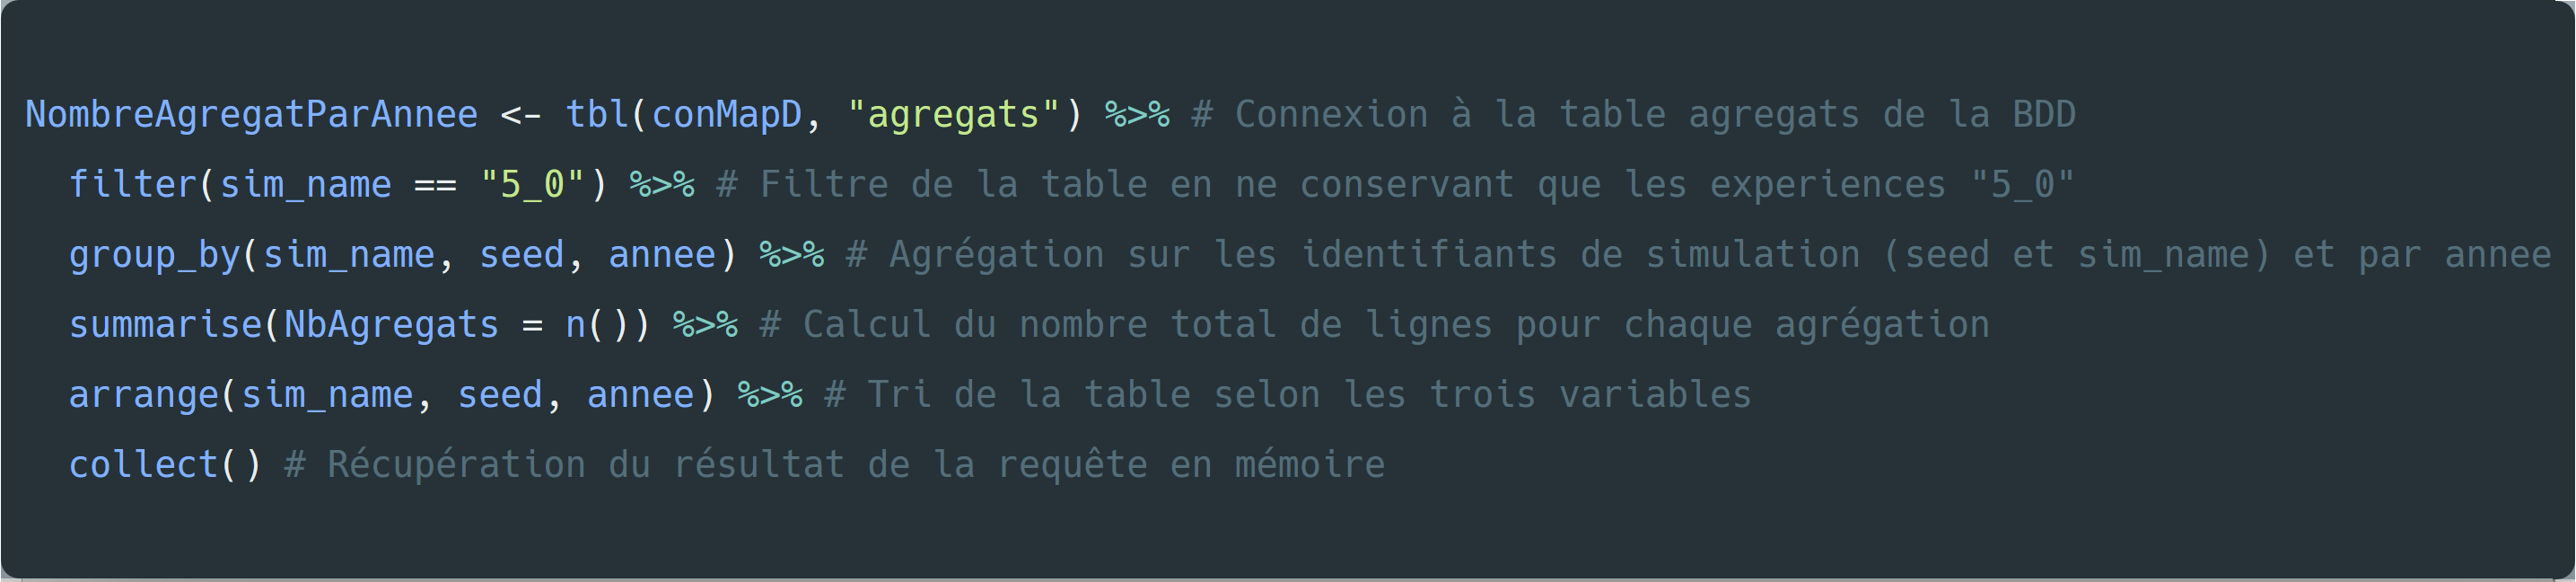
\includegraphics[width=\linewidth]{img/dplyr_cut.png}}
\hspace{5pt}
\subfloat[Traduction du code source \textsf{dplyr} en \textsf{SQL}]{\label{subfig:exemple-dplyr-SQL}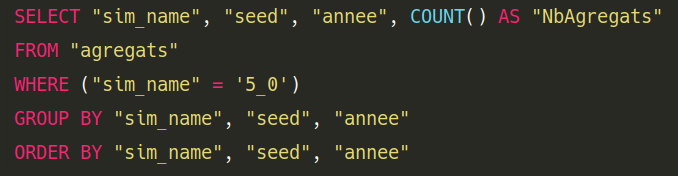
\includegraphics[scale=.35]{img/SQL_Sublime.png}}
\caption{Un exemple de manipulation de données stockées dans un SGBD depuis R. On y interroge la table des agrégats de population pour calculer le nombre moyen d'agrégats par année de simulation.}
\label{fig:dml-simedb}
\end{figure}

\clearpage
\paragraph*{Création de graphiques avec \textsf{ggplot2} et la \og \textit{grammar of graphics}\fg{}}

\paragraph*{}
\begin{wrapfigure}{l}{.42\linewidth}
\centering
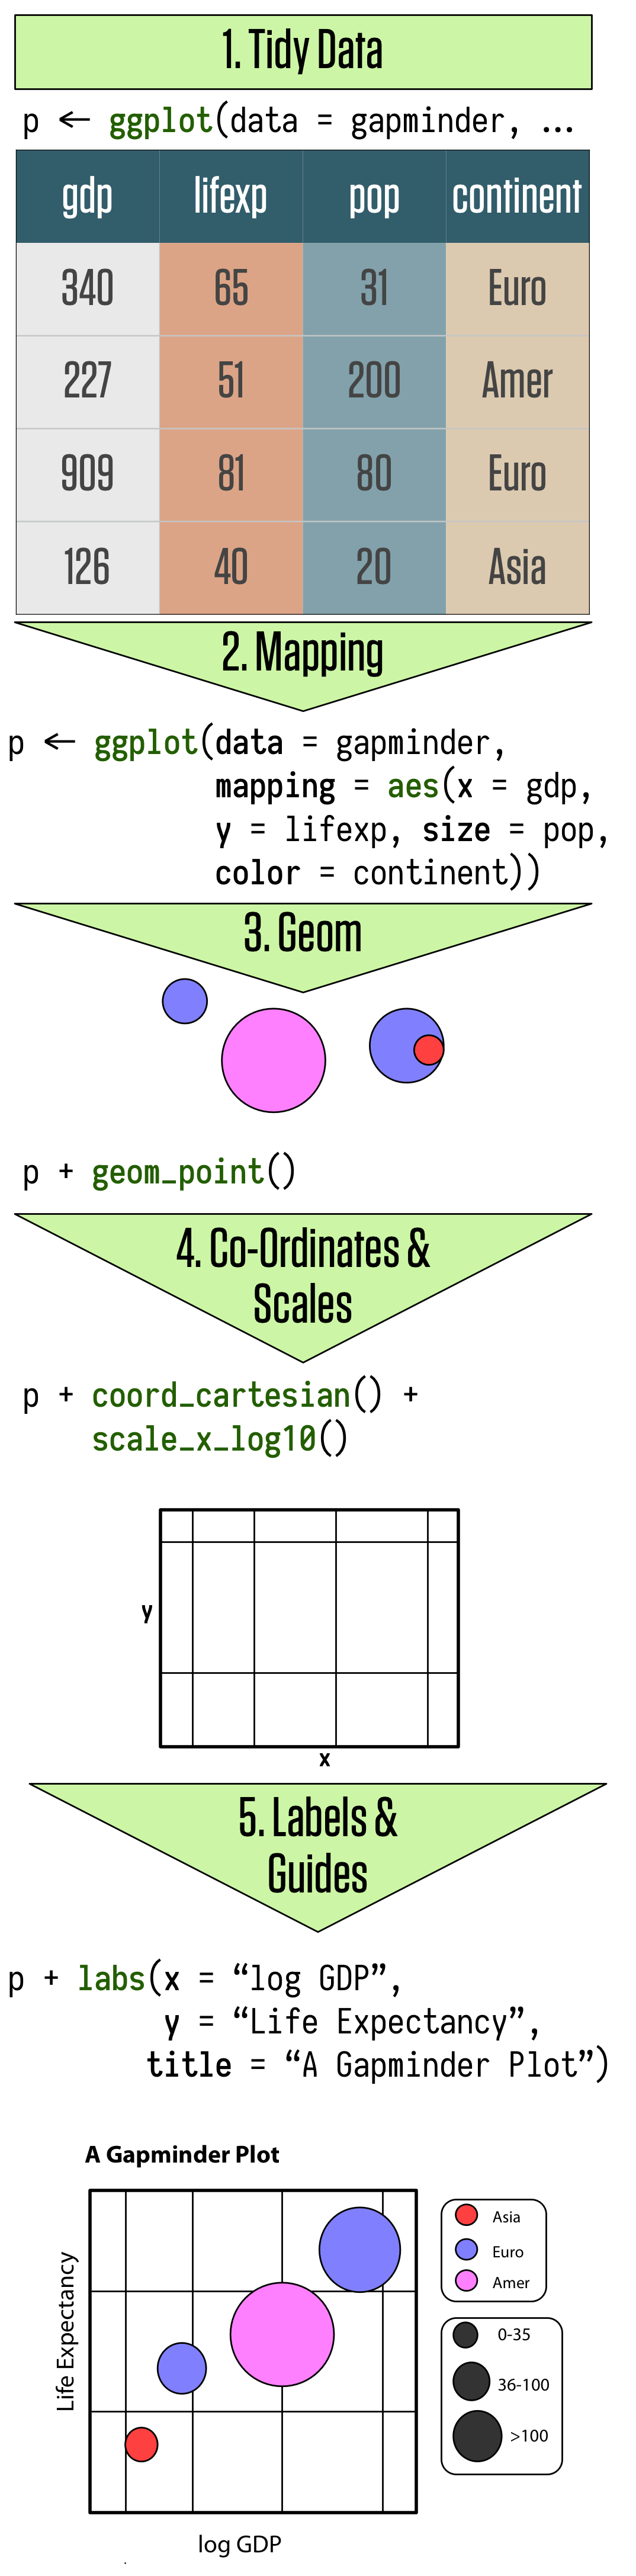
\includegraphics[width=.92\linewidth]{img/ch-03-ggplot-flow-vertical.png}
\caption{Représentation des éléments de grammaire de \textsf{ggplot2}, tiré de \cite{healy_data_2018}.\\
\hl{Ré-organiser proprement le graphique}%
}
\label{fig:socviz-ggplot2}
\end{wrapfigure}
Une fois les données pré-traitées, encore est-il nécessaire de construire les indicateurs graphiques de sortie de simulation.
Pour cela, il existe de nombreux \textit{packages} pour R dédiés à la représentation graphique.

L'un des \textit{packages} les plus utilisés, \textsf{ggplot2} \autocite{wickham_ggplot2_2016}, met en œuvre une syntaxe assez adaptée à nos contraintes : ce \textit{package} est conceptuellement fondé sur la \og \textit{grammar of graphics}\fg{}, c'est-à-dire une vision modulaire et très structurée de la conception graphique, pensée par Leland Wilkison \autocite{wilkinson_grammar_2006}.
La logique, assez familière pour un utilisateur de Systèmes d'Information Géographique (SIG), consiste à penser une représentation graphique comme un ensemble de couches (\textit{layers}), qui se superposent, se complètent, et sont toutes basées sur une source de données.
Les différentes composantes des données (variables par exemple) sont associées à des composantes graphiques de base (abscisse, ordonnée, taille, couleur \ldots), formant ainsi une \og cartographie\fg{} (\textit{mapping}) des données avec les composants graphiques (voir \cref{fig:socviz-ggplot2}).

Pour SimEDB, l'un des intérêts principaux de créer les indicateurs graphiques est justement cette grammaire, extrêmement structurée, qui permet donc de ré-utiliser largement les codes-sources écrits pour un indicateur et de les adapter aisément à d'autres indicateurs.
Par exemple, de nombreux indicateurs de sortie de SimFeodal montrent l'évolution du nombre d'agents au cours des années de simulation (\cref{fig:exemple-ggplot2-simedb}).
Ce type de graphique est rapide à produire avec \textsf{ggplot2} -- il ne requiert que quelques lignes de code (\cref{subfig:exemple-ggplot2-R}) --,
et en changeant le tableau de données en entrée (créé dans \cref{subfig:exemple-dplyr-R}), reproduit exactement le même type de graphique pour, par exemple, un autre type d'agent.
Le \textit{package} \textsf{ggplot2} répond tout à fait aux contraintes de modularité exposées plus haut, et permet de factoriser le code-source, ce qui garanti une maintenance plus rapide et une meilleure robustesse de l'application dans son ensemble.

\clearpage

\begin{figure}[H]
\centering
\hspace{5pt}
\subfloat[Code source R avec le \textit{package} \textsf{ggplot2}]{\label{subfig:exemple-ggplot2-R}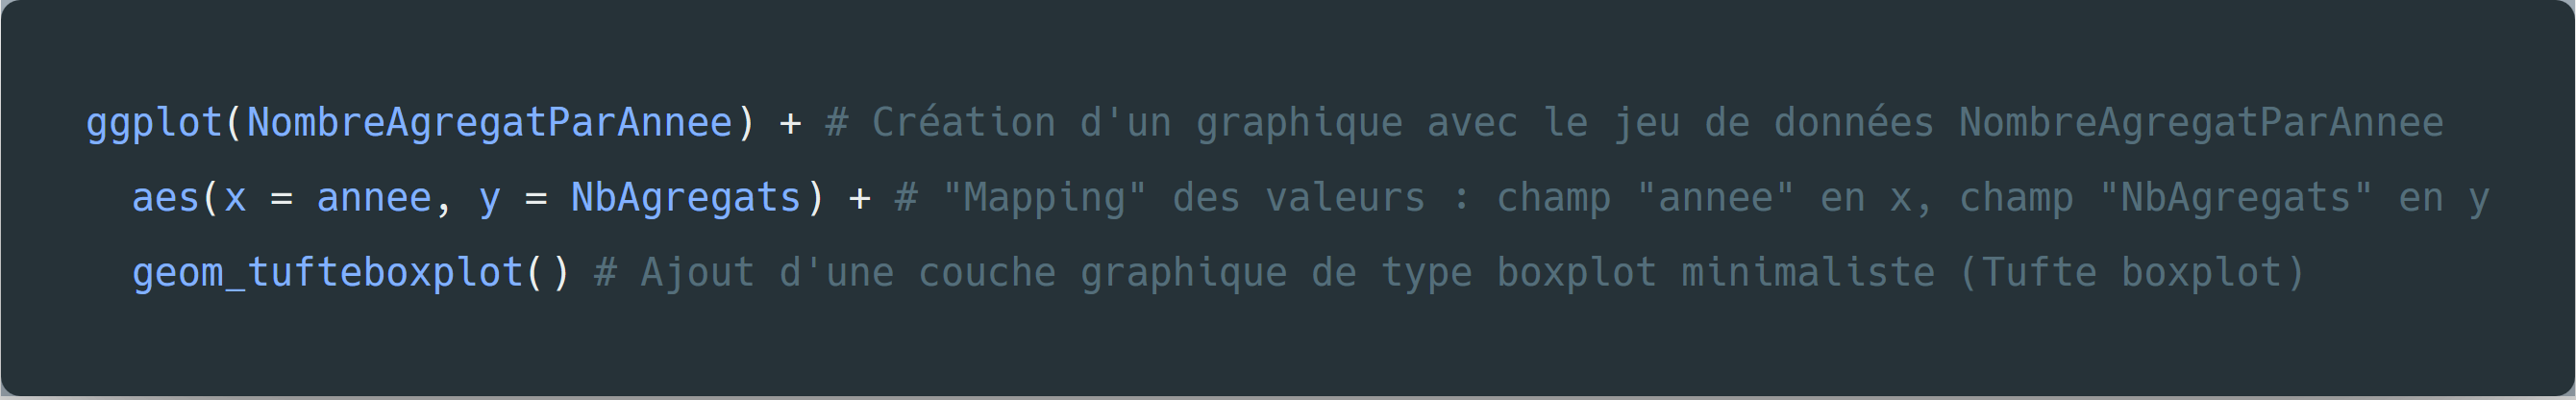
\includegraphics[scale=.15]{img/ggplot2.png}}
\hspace{5pt}
\subfloat[Graphique généré]{\label{subfig:exemple-ggplot2-plot}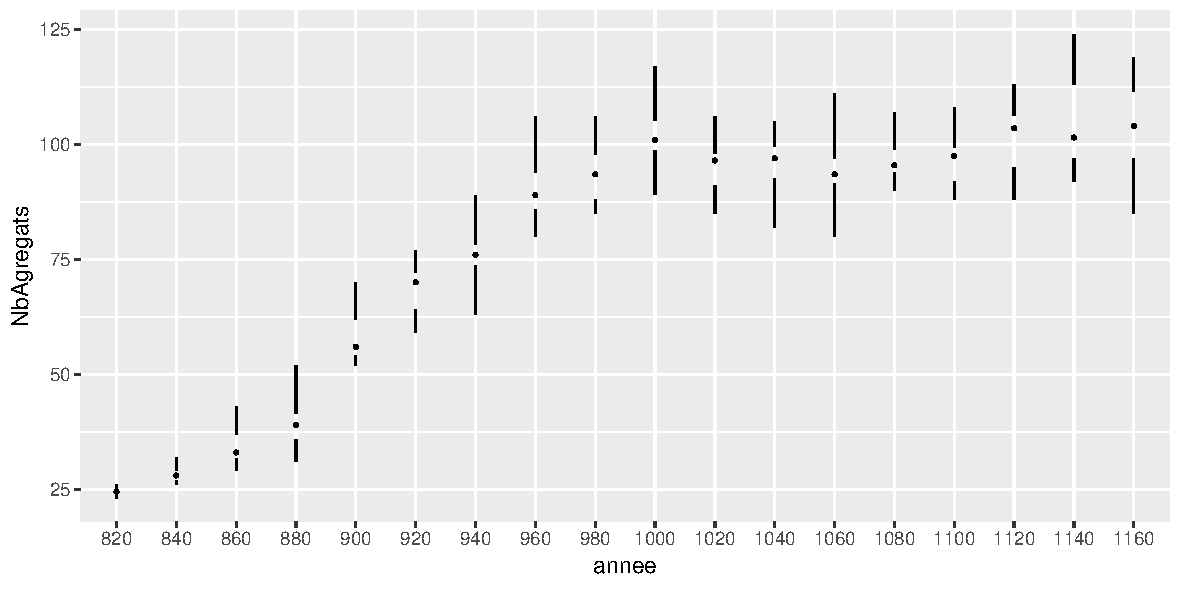
\includegraphics[width=\linewidth]{img/chap5_exemple_indicateur.pdf}}
\caption{Un exemple de manipulation de données stockées dans un SGBD depuis R.}
\label{fig:exemple-ggplot2-simedb}
\end{figure}

\paragraph*{Fluidifier les étapes de rendu : le \og pipeline de visualisation\fg{}}\label{par:visualisation-pipeline}


\Cite{dos_santos_gaining_2004} ont conceptualisé et schématisé l'ensemble des étapes nécessaires à la construction d'une visualisation, depuis les données brutes jusqu'à l'image finale, au sein d'un \og pipeline\fg{} de la visualisation (\cref{subfig:visualisation-pipeline}).

Dans la chaîne de traitement la plus classique, ces étapes s'effectuent au sein de différents logiciels, chacun dédiés à une tâche. Dans le domaine des utilisateurs de SIG, on retrouve par exemple fréquemment une préparation des données dans un tableur, un import dans un logiciel SIG qui va être chargé de la cartographie, puis un export vers un logiciel de dessin vectoriel afin de réaliser la mise en page.
À chaque changement de logiciel, il est nécessaire d'exporter les données produites, puis de les ré-importer dans le logiciel suivant.

A contrario, le propre de l'utilisation d'un langage de programmation plutôt que d'un outil graphique est de pouvoir automatiser et intégrer l'ensemble de ces étapes.
L'utilisation de \textsf{R} comme langage de développement de SimEDB nous permet ainsi de développer une unique chaîne de traitement, qui ne requiert aucun import/export de données, et peut donc être consolidée, vérifiée et surtout ré-employée \textit{ad libitum}.

L'enchaînement des \textit{packages} employées dans SimEDB est présenté dans la \cref{subfig:visualisation-pipeline-simedb}, et le code-source correspondant à l'exemple développé dans cette sous-partie dans la \cref{fig:visualisation-pipeline-exemple}.

\begin{figure}[H]
\centering
\hspace{5pt}
\subfloat[\og \textit{The Visualisation Pipeline}\fg{}, de \cite{keim_mastering_2010}, p.92, d'après \cite{dos_santos_gaining_2004}, p. 314 ]{\label{subfig:visualisation-pipeline}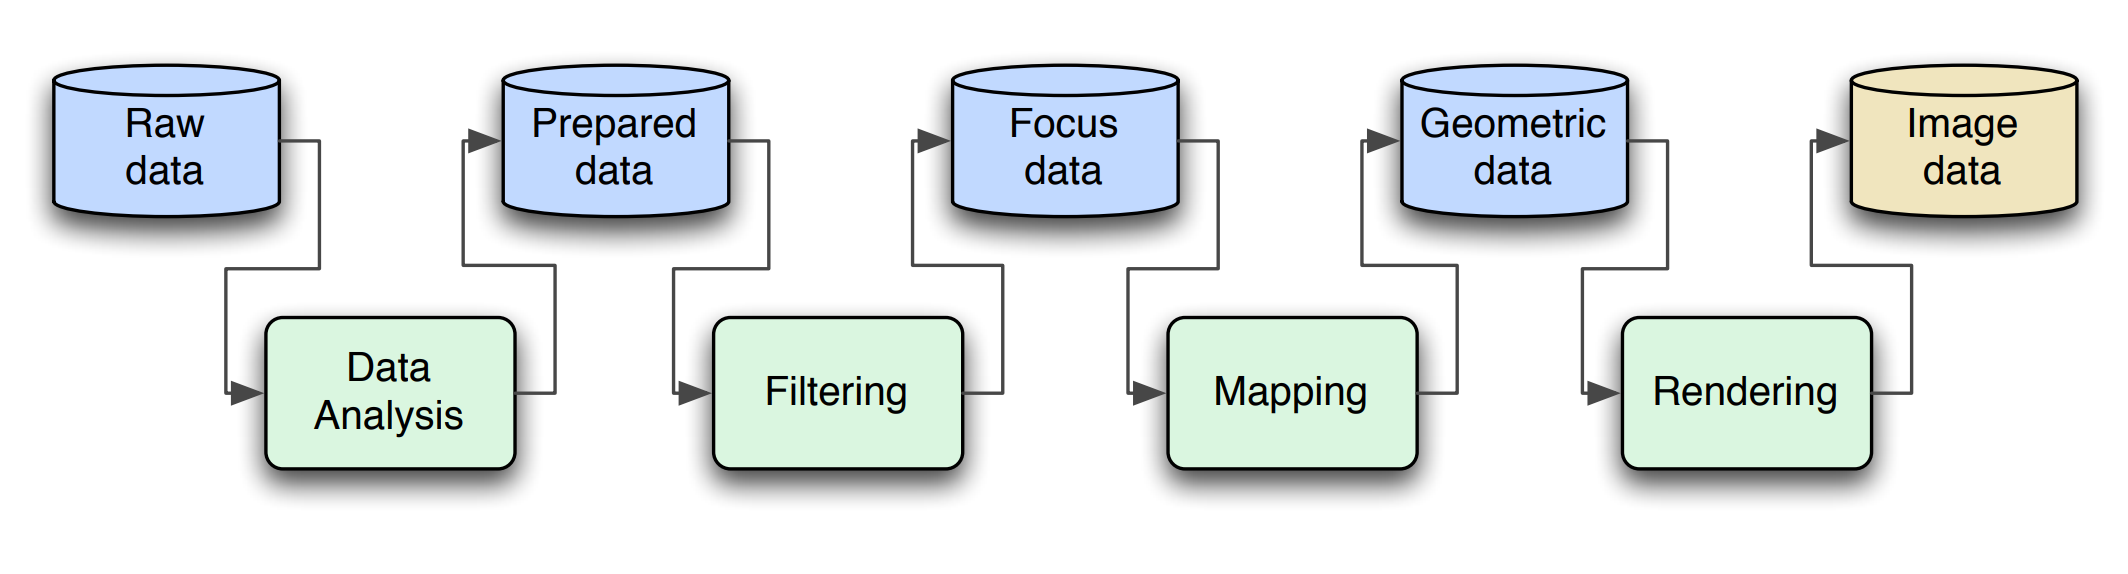
\includegraphics[width=\linewidth]{img/Visualisation_Pipeline_p92.png}}
\hspace{5pt}
\subfloat[Technologies utilisées dans SimEDB.]{\label{subfig:visualisation-pipeline-simedb}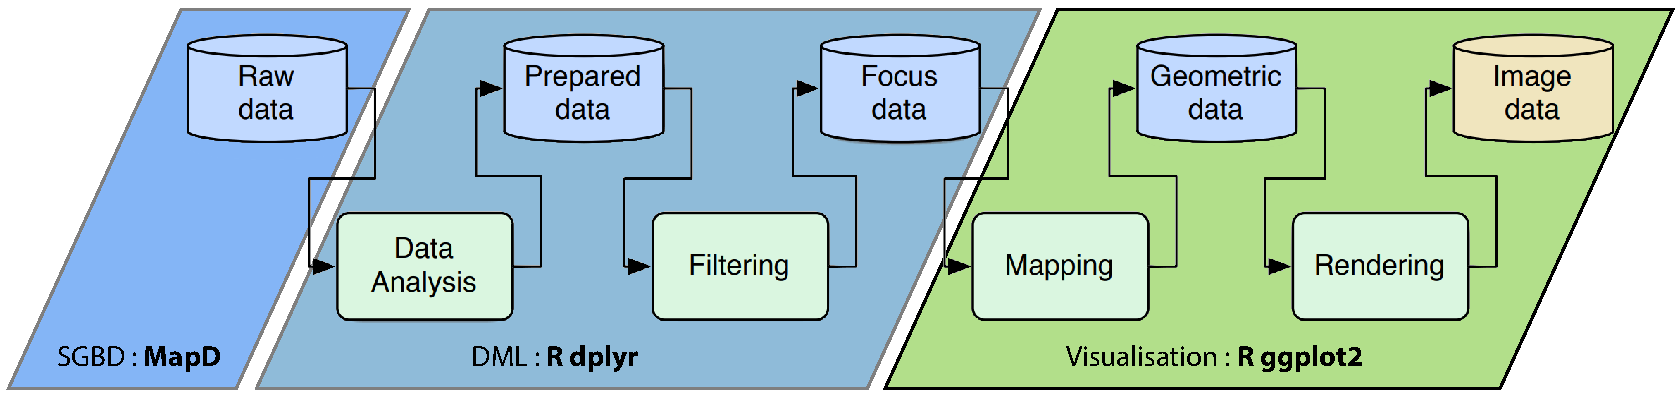
\includegraphics[width=\linewidth]{img/Visualisation_Pipeline_SimEDB.pdf}}
\hspace{5pt}
\subfloat[Une implémentation d'un exemple de pipeline de visualisation pour construire un indicateur dans SimEDB]{\label{subfig:exemple-pipeline-simedb}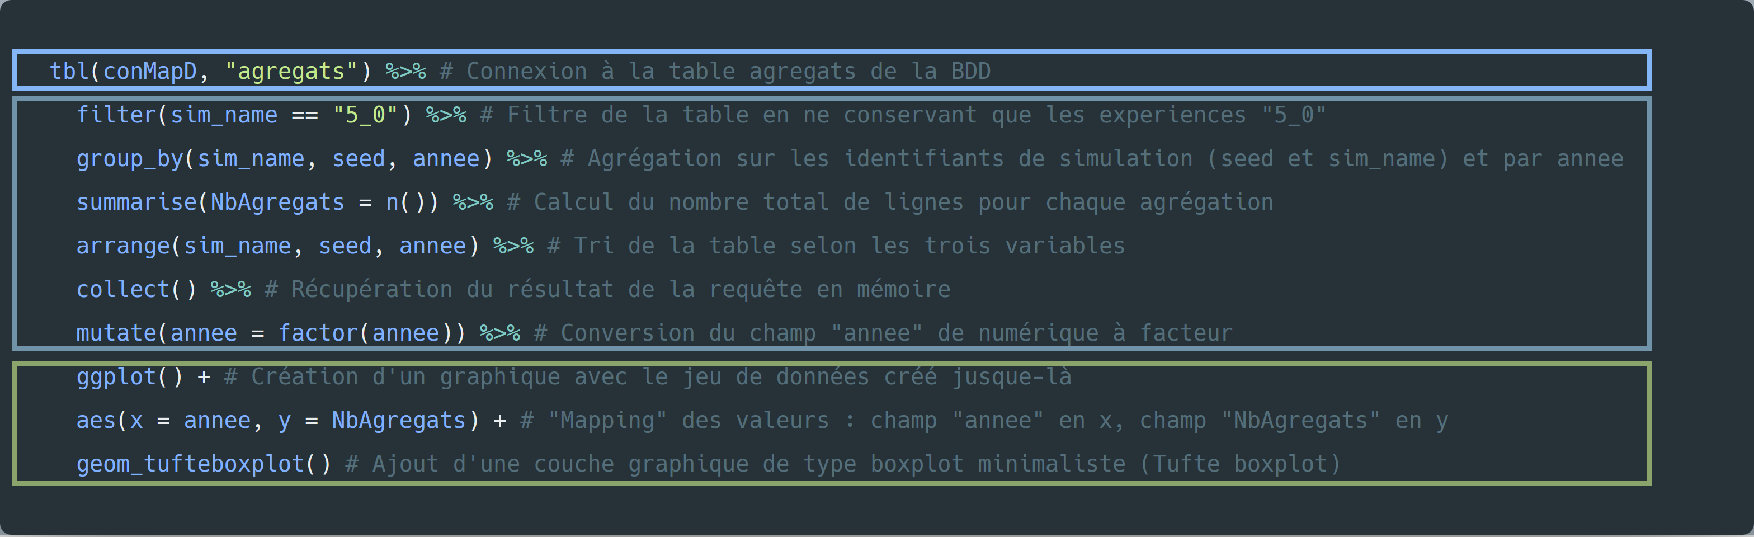
\includegraphics[width=\linewidth]{img/simedb_pipeline_R.pdf}}
\caption{\og \textit{Visualisation Pipeline}\fg{} et son implémentation dans SimEDB, en \og connectant\fg{} les codes des \cref{fig:dml-simedb,fig:exemple-ggplot2-simedb}.}
\label{fig:visualisation-pipeline-exemple}
\end{figure}

\paragraph*{Modulariser les fonctions}

\textsf{Shiny}, en tant qu'outil de création d'interface graphique, bénéficie aussi d'un avantage important en matière de conception d'application web : comme ce \textit{package} est basé sur un langage de programmation modulaire, on peut logiquement créer et ré-utiliser des \og briques d'interfaces\fg{} modulaires.
Par l'utilisation de modules\footnote{\href{https://shiny.rstudio.com/articles/modules.html}{https://shiny.rstudio.com/articles/modules.html}}, il est possible de définir un ensemble d'éléments graphiques adaptatifs et de ré-utiliser tel quel cet ensemble.

Dans l'interface de SimEDB, par exemple, les indicateurs graphiques sont toujours présentés de la même manière, avec l'indicateur à gauche et des outils de téléchargement et de notation de l'indicateur sur la droite.
En termes de code, les deux indicateurs comparés dans la \cref{fig:simedb-modules} sont strictement identiques : seul un paramètre varie dans l'appel aux modules, ici les filtres appliqués sur les données.
Cela permet donc d'une part de minimiser la taille du code, mais surtout, avec la généricité apportée, de faciliter de manière considérable l'ajout ou la modification d'indicateurs.

\begin{figure}[H]
\centering
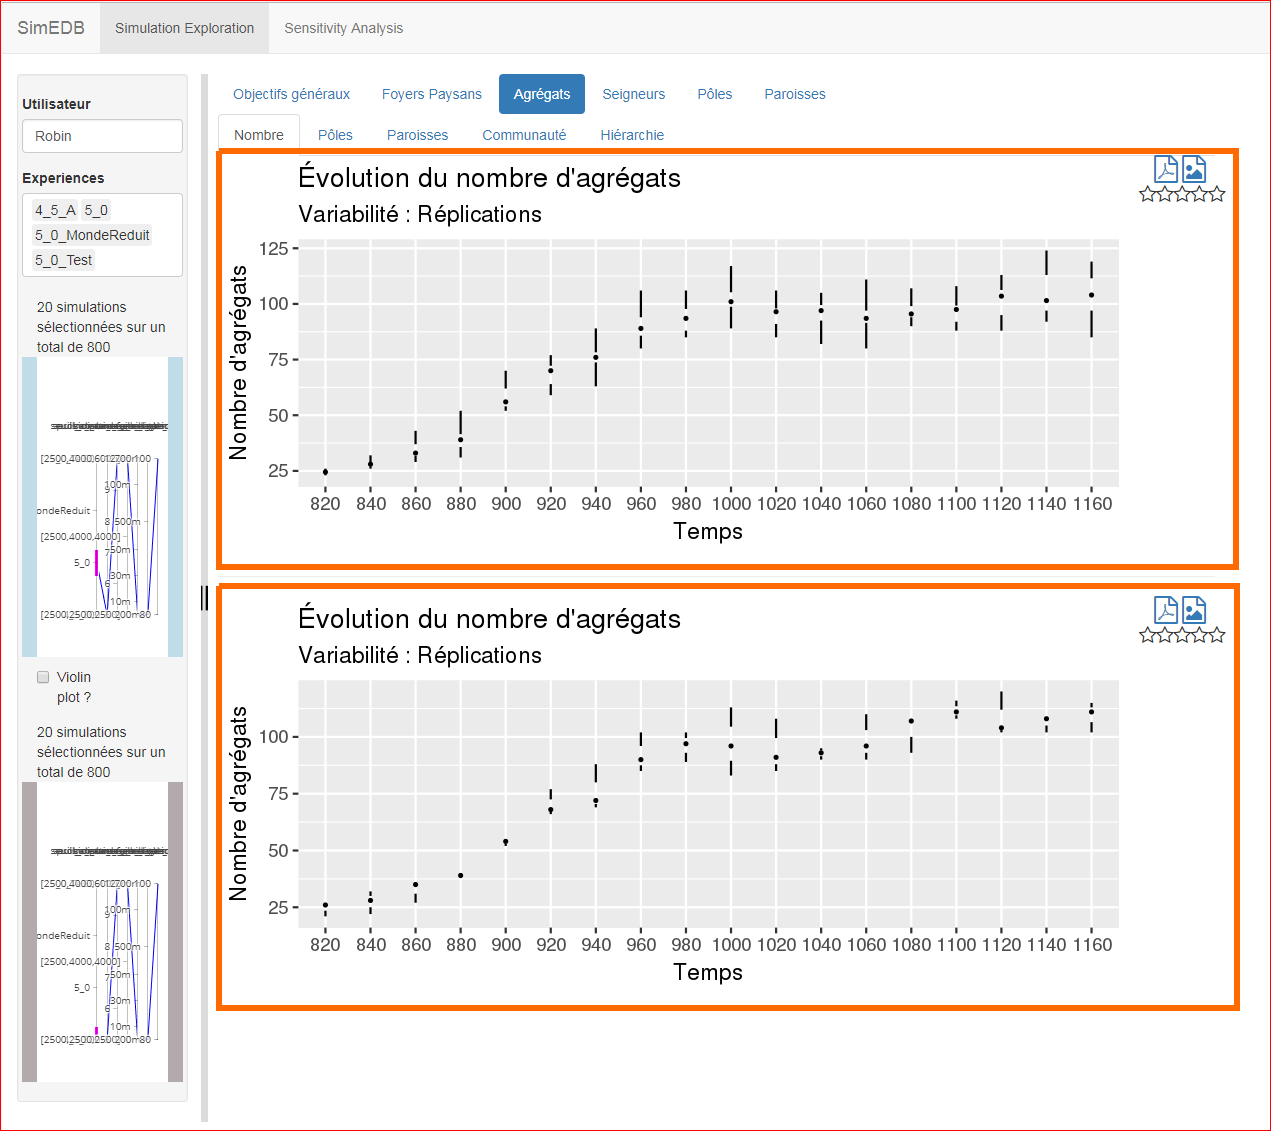
\includegraphics[width=\linewidth]{img/SimEDB_modules.png}
\caption{Une conception modulaire. Les deux éléments graphiques encadrés sont créés par un même \og module\fg{} dont les arguments varient.}
\label{fig:simedb-modules}
\end{figure}


\subsubsection{Choix de l'organisation visuelle}

Les différentes étapes de construction d'une plate-forme d'exploration (\cref{sec:explorer-sorties-simfeodal} : \cnameref{sec:explorer-sorties-simfeodal}) ont conduit à une organisation sous forme de \textit{dashboard} interactif.
La forme de ce \textit{dashboard} a évolué tout au long de l'apparition de nouveaux besoins, pour aboutir sur une organisation mono-page, pensée autour de la consultation d'indicateurs de sorties, qui devaient permettre de comparer des expériences différentes sélectionnées au moyen de graphiques en coordonnées parallèles.
Le choix d'un outil dédié à la comparaison, plus qu'à la visualisation des résultats d'un unique ensemble de simulations, entraîne nécessairement des répercussions en matière de présentation visuelle -- d'interface graphique -- des éléments permettant de mener cette comparaison.
Depuis la première plate-forme aboutie -- SimVADB (voir \cref{fig:simvadb_dashboard}, \cpageref{fig:simvadb_dashboard}) --, l'interface graphique a donc fortement évolué.

\paragraph*{Une comparaison verticale}

En premier lieu, on peut remarquer que les \og contrôleurs\fg{}, c'est-à-dire les graphiques interactifs en coordonnées parallèles ainsi que de nouveaux menus de sélections (\cref{fig:simedb-sidebar}) ne sont plus dans la partie supérieure de l'interface, mais dans la partie latérale de l'application.

Le choix prédominant à cette modification est la volonté de comparaison : dans SimVADB, on pouvait déjà comparer deux graphiques, mais ceux-ci étaient alors côte-à-côte.
Étant donné que l'axe des ordonnées est dépendant de chaque graphique -- on ne peut attribuer de limites communes à chaque graphique sans avoir à recalculer chacun des indicateurs à chaque changement de sélection de l'un ou de l'autre --, une comparaison visuelle des positions en ordonnées des courbes et marqueurs n'a pas véritablement de sens.
Au contraire, le plus souvent, l'axe des abscisses est fixe : qu'il représente le temps (nombre d'agrégats par pas de temps\ldots), une discrétisation de valeurs continues (composition en attracteurs des pôles\ldots), ou encore les différentes modalités d'une variable (détail du déplacement des foyers paysans\ldots), l'étendu et la composition des éléments en abscisse est généralement prévisible.

Avec un axe \og fixe\fg{}, il est donc opportun de mener la comparaison visuelle sur cet axe, et donc d'aligner les graphiques sur celui-ci. L'organisation des différents indicateurs est donc verticale plutôt qu'horizontale.

\begin{figure}[H]
\centering
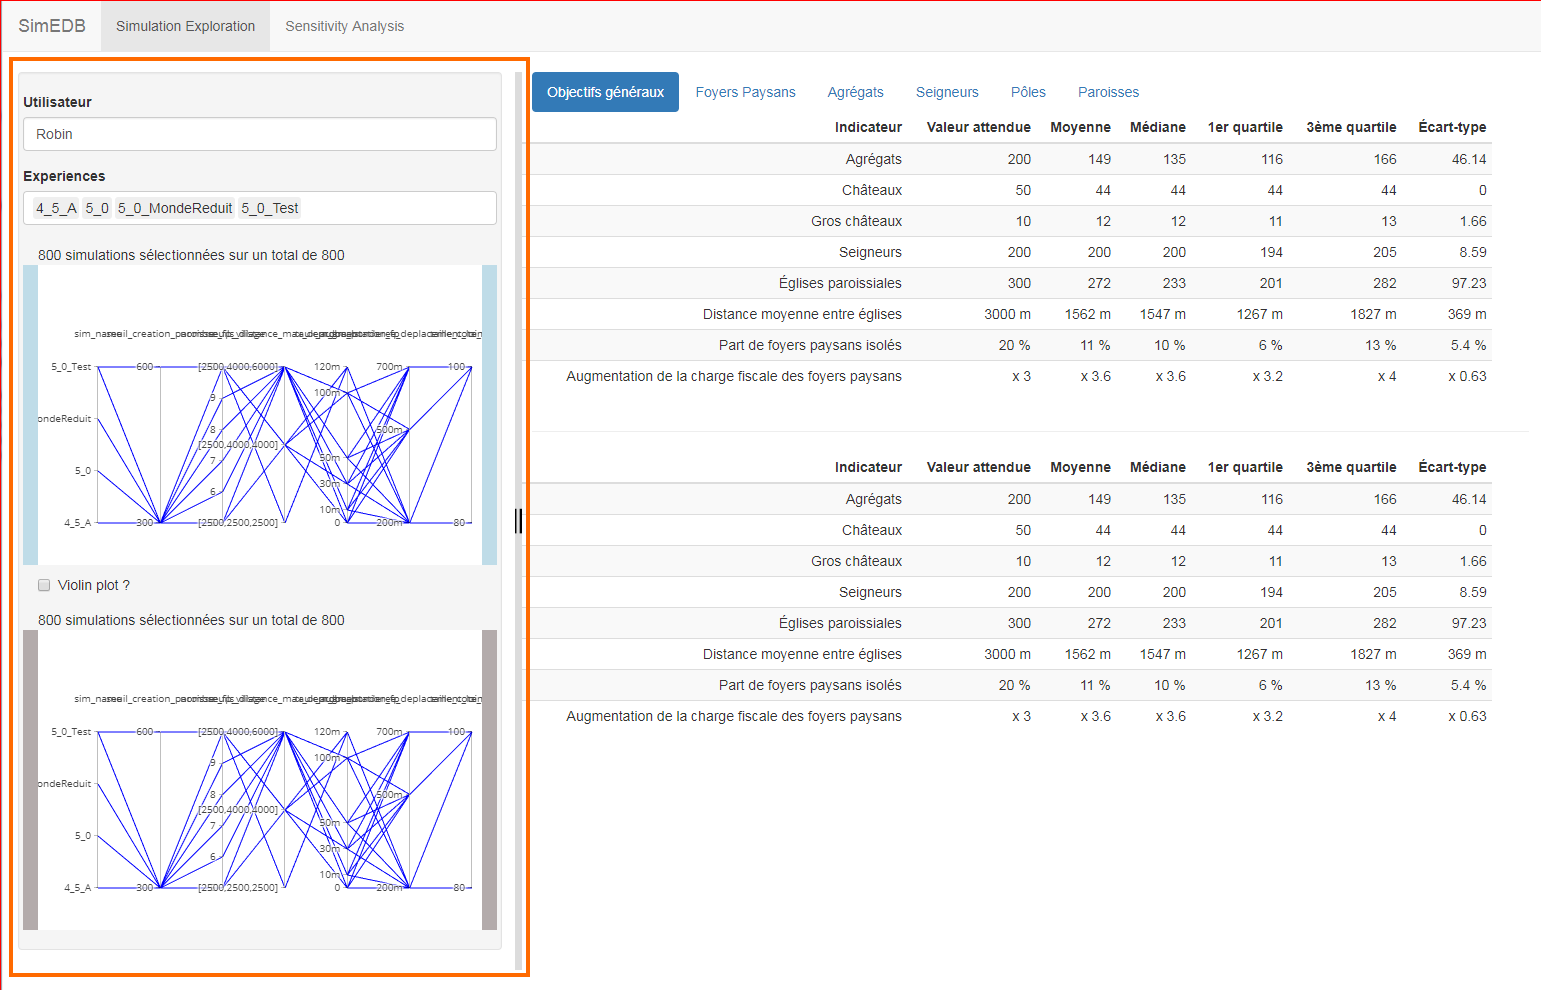
\includegraphics[width=\linewidth]{img/SimEDB_sidebar_cut.png}
\caption{La barre de contrôleurs dans l'interface de SimEDB}
\label{fig:simedb-sidebar}
\end{figure}

Afin que la sélection des simulations à explorer soit intuitive, les contrôleurs doivent donc être alignés face à cet agencement vertical des indicateurs, et dès lors, verticalisés eux aussi.

Pour bien différencier visuellement ce qui relève d'un affichage et ce qui requiert une interaction, les contrôleurs s'inscrivent dans un panneau dédié, grisé, ce qui constitue presque un standard dans les interfaces modernes d'applications interactives.

\paragraph*{Onglets et sous-onglets}

Comme dans SimVADB (\cref{subsubsec:simvadb}, \cpageref{subsubsec:simvadb}), on a choisi de conserver une navigation entre indicateurs par un systèmes d'onglets imbriqués : un premier niveau d'onglets permet d'accéder au type d'agents concernés par les indicateurs, et un second niveau permet de sélectionner spécifiquement l'indicateur choisi.
On aurait pu privilégier une vision globale, par exemple en affichant d'un coup, pour chaque type d'agents, l'ensemble des indicateurs concernés.
Sur des écrans de grande dimension, cela aurait permis d'embrasser du regard les résultats propres à chaque type d'agent bien plus rapidement, et d'accélérer d'autant l'évaluation de simulations ou leur comparaison.
La majorité des utilisateurs potentiels de SimEDB consultent toutefois l'application sur des ordinateurs portables, dotés d'écran réduits et d'une résolution faible.
L'encombrement visuel est alors atteint rapidement, et mieux vaut présenter un indicateur à la fois : la démarche visuelle sera plus longue, mais ne sera pas gênée ou faussée par des graphiques de dimension trop réduites qui peuvent induire des erreurs de lecture.

L'organisation des onglets en eux-mêmes pose aussi une question importante : vaut-il mieux organiser la consultation par type d'agent, ou plutôt, hiérarchiquement, selon la catégorie de processus examinée (\hl{à corriger une fois fixé sur le terme}, \hl{faire ref au chap3}), par exemple en respectant l'ordre de consultation des indicateurs déterminé ?

Les deux approches présentent des avantages, mais nous avons choisi de rendre l'utilisation de SimEDB plus intuitive à tous, c'est-à-dire en organisant les indicateurs par type d'agents, plutôt qu'efficace, pour les utilisateurs habitués qui auraient bénéficié d'une organisation structurée hiérarchiquement.

\subsubsection{Choix des modes d'interactions}

Avant même la conception de SimEDB, avec la plate-forme SimVADB, nous avions décidé de baser la sélection des simulations sur des graphiques en coordonnées parallèles interactifs (\cref{subsec:explo-interactive} : \cnameref{subsec:explo-interactive}).
La logique d'ensemble du filtrage de simulations restant la même, il n'était pas nécessaire de modifier ce choix pour SimEDB.

L'accumulation d'expériences, reposant sur les variations de paramètres différents, ainsi que la démultiplication des paramètres du modèle SimFeodal ayant accompagné son paramétrage, ont pourtant demandé de reconsidérer l'usage de ces graphiques interactifs.
Là où seuls quelques paramètres étaient mobilisés auparavant, les graphiques en coordonnées parallèles reposaient sur peu d'axes.
Avec l'augmentation du nombre d'axes, le graphique en coordonnées parallèle est rapidement devenu illisible faute à une surcharge graphique due au recouvrement des axes.

\paragraph*{Réduire la surcharge visuelle des graphiques en coordonnées parallèles}

La première mesure pour y remédier a été de filtrer les paramètres affichés : nul besoin d'afficher un axe correspondant à un paramètre qui n'est jamais manipulé dans les expériences.
Plutôt que de définir les paramètres \og utiles\fg{}, et donc d'avoir à les redéfinir dans l'application à chaque ajout d'expérience qui reposerait sur la variation d'un paramètre différent, nous avons fait en sorte que cette discrimination des paramètres \og actifs\fg{} soit exécutée de manière automatique :
quand SimEDB est lancé, une requête est exécutée sur la table des paramètres pour identifier ceux qui présentent plusieurs modalités et ceux qui n'en ont qu'une.
Seuls sont alors affichés les paramètres de la première catégorie, car eux-seuls présent un intérêt à être discriminés.

Ce faisant, le nombre de  paramètre affichés devient plus réduit, et permet d'afficher leurs intitulés plutôt que de faire appel à une table de correspondance comme dans SimVADB.
L'automatisation de ce traitement permet de plus de ne pas avoir à changer quoi que ce soit à la plate-forme lors d'ajouts ou de suppressions de simulations de la base de données, ce qui concoure à l'objectif d'indépendance aux données de la plate-forme d'exploration.

\paragraph*{Pré-filtrer les simulations}

Au fur et à mesure du paramétrage puis de la calibration de SimFeodal, les expériences ont tout de même continué à mobiliser de plus en plus de paramètres différents.
Pour réduire la quantité d'information représentée et améliorer en conséquence \og l'expérience utilisateur\fg{}, nous avons ajouté un filtre, moins visuel que les graphiques en coordonnées parallèle, qui permet toutefois de restreindre le nombre de simulations affichées à partir de leur dénomination.
Plutôt que de cibler des valeurs spécifiques de paramètres, l'idée est donc de soustraire des choix possibles des expériences entières.
Pour SimEDB, on a donc ajouté un pré-filtrage, sous forme de \og boîte de sélection\fg{} (\textit{select input}, \cref{fig:simedb-prefilter}), qui interroge la base de données directement pour connaître les différents intitulés de simulations et agit comme un premier filtre réduisant donc les simulations interrogées dans les graphiques en coordonnées parallèles.

\begin{figure}[H]
\centering
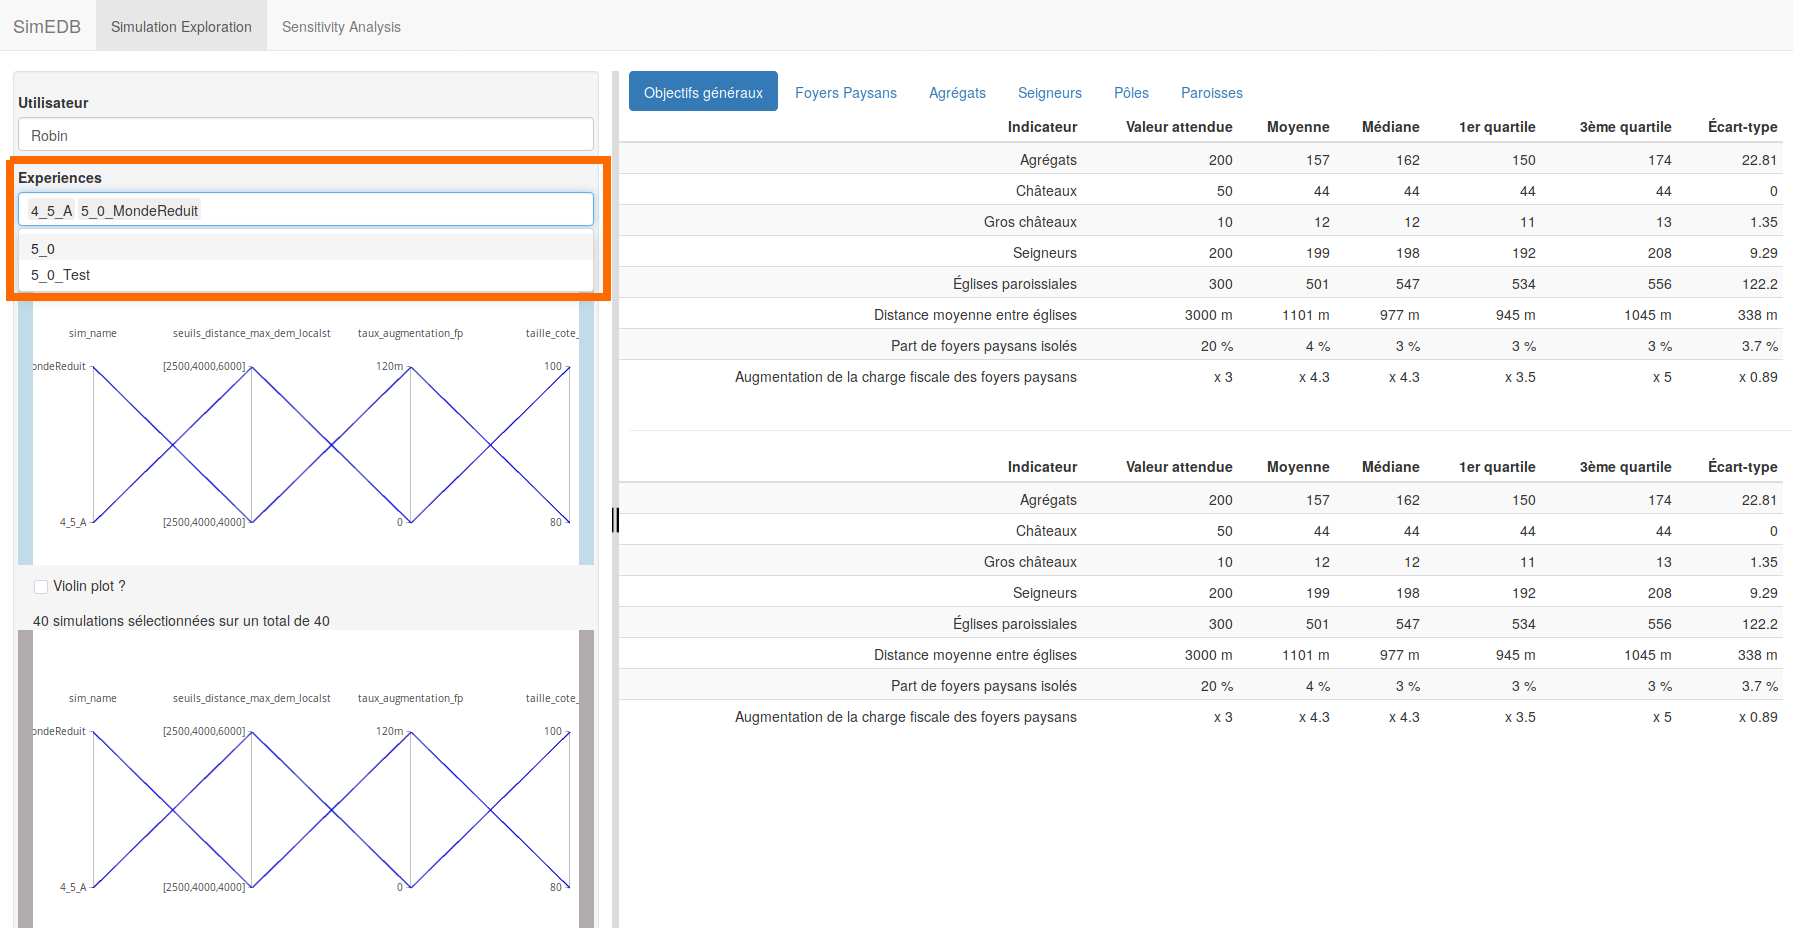
\includegraphics[width=\linewidth]{img/SimEDB_prefiltrage.png}
\caption{Le menu de sélection des expériences qui permet un pré-filtrage des expériences à partir de leur nom}
\label{fig:simedb-prefilter}
\end{figure}

\paragraph*{Optimiser l'occupation de l'espace visuel}\label{par:simedb-resize-parcoords}

En dépit de ces différentes techniques visant à minimiser le nombre d'axes affichées dans les graphiques en coordonnées parallèles, la place prise par ces graphiques reste importante, en particulier quand on décide de ne pas diminuer la taille des éléments de légende afin de conserver leur lisibilité.
Quand l'application est consultée sur un écran de taille faible, l'appréhension de l'ensemble des informations présentes dans l'interface pose ainsi un véritable problème.

En réfléchissant aux séquences d'usages, par les utilisateurs, de SimEDB, on a pu comprendre que le mode d'utilisation le plus classique était de bien considérer le filtrage à effectuer sur les graphiques en coordonnées parallèles, en y consacrant un temps certain, avant de comparer longuement les différents indicateurs de la sélection.
Il n'est donc que rarement fait usage de multiples filtres successifs sur un seul indicateur, dans une approche plus exploratoire donc, mais plutôt d'évaluations complètes de simulations choisies.

Il n'est alors plus indispensable de consacrer une part importante de l'espace aux zones interactives (le panneau de contrôle), ou du moins, pas pendant l'ensemble de la période d'évaluation des simulations.

Un outil de redimensionnement a alors été ajouté à SimEDB, permettant, par glisser-déposer, de modifier la largeur occupée par le panneau de contrôle en l'adaptant à chaque moment au besoin de visualisation.
La \cref{fig:resizing} montre ainsi une succession d'états : en début d'exploration, l'utilisateur va augmenter la taille du panneau de contrôle pour augmenter la lisibilité des graphiques en coordonnées parallèles et effectuer une sélection plus simplement.
Une fois la sélection effectuée, il pourra alors re-diminuer la largeur du panneau afin d'augmenter la zone disponible, et donc la taille, pour les indicateurs de sorties de simulation. 

\begin{figure}[H]
\hspace*{\fill}%
\begin{minipage}[t]{.49\linewidth}
\centering
\vspace{0pt}
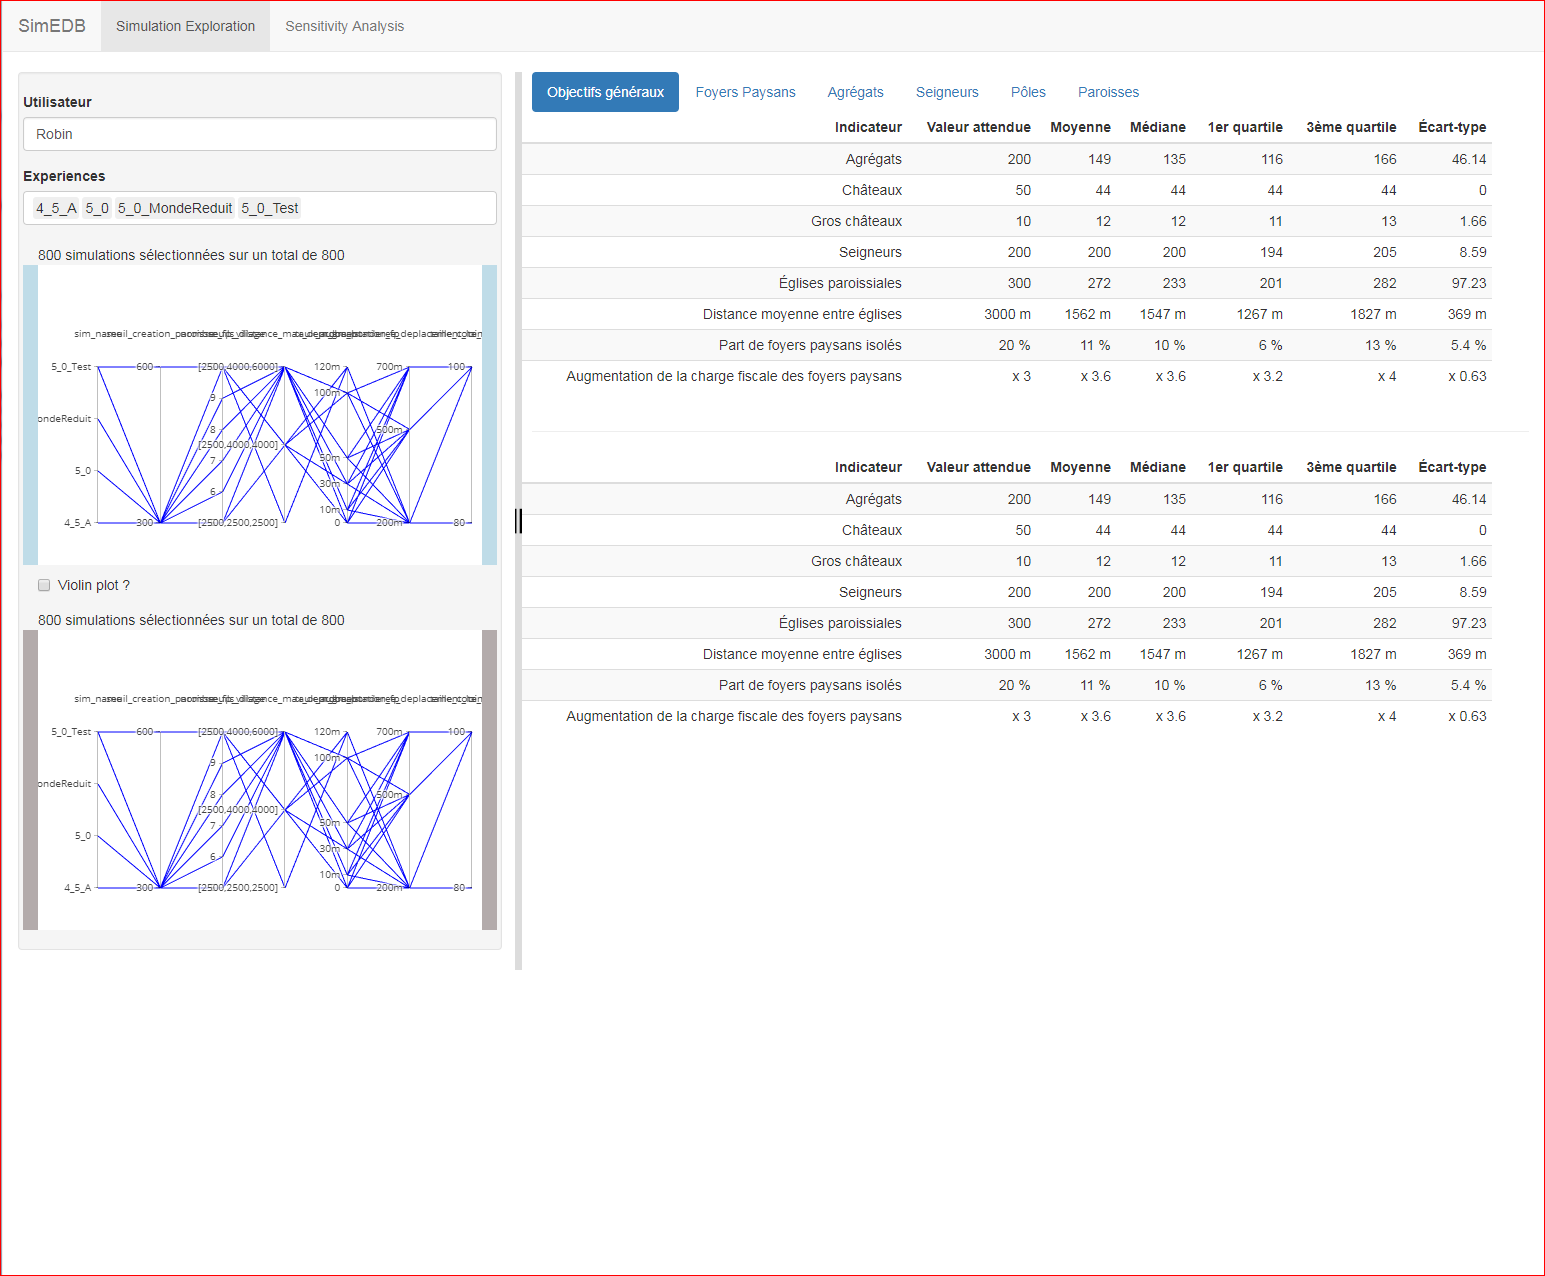
\includegraphics[width=\linewidth]{img/SimEDB_base.png}
\end{minipage} \hfill
\begin{minipage}[t]{.49\linewidth}
\centering
\vspace{0pt}
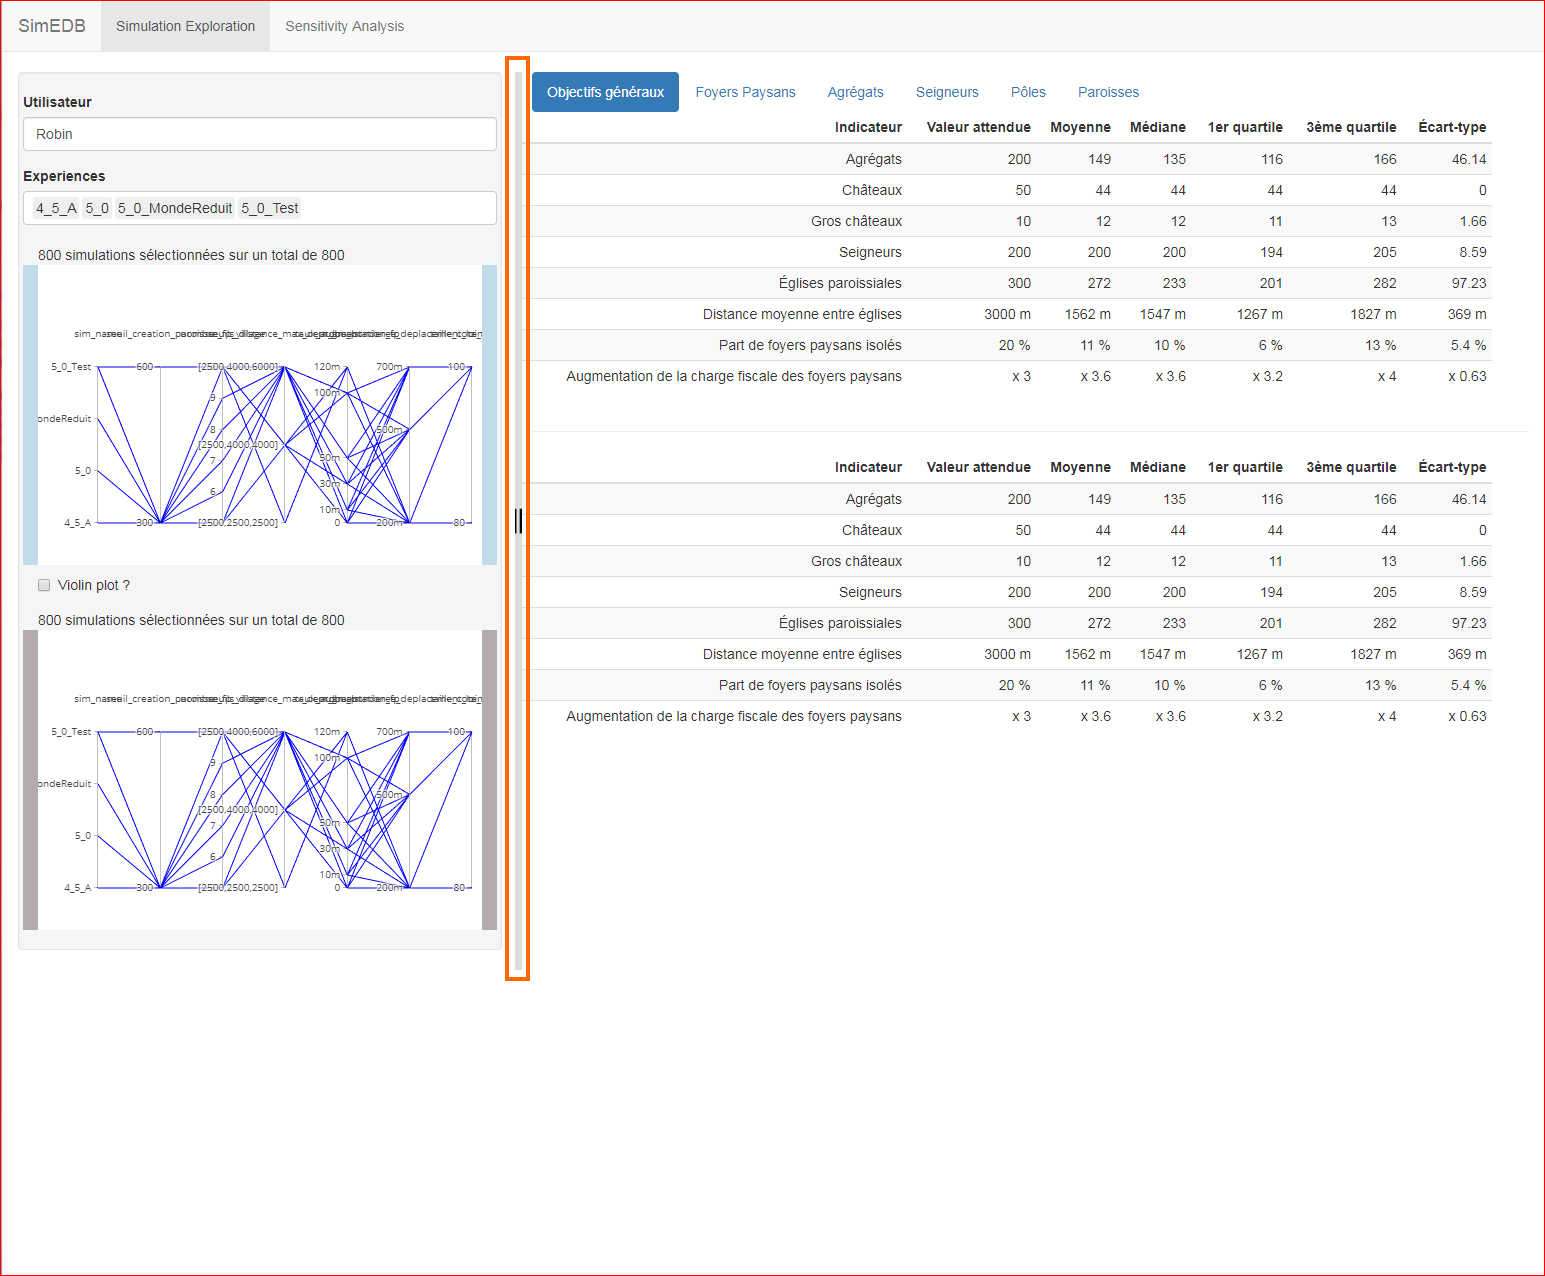
\includegraphics[width=\linewidth]{img/SimEDB_resize.png}
\end{minipage} \hfill
\begin{minipage}[b]{.49\linewidth}
\centering
\vspace{0pt}
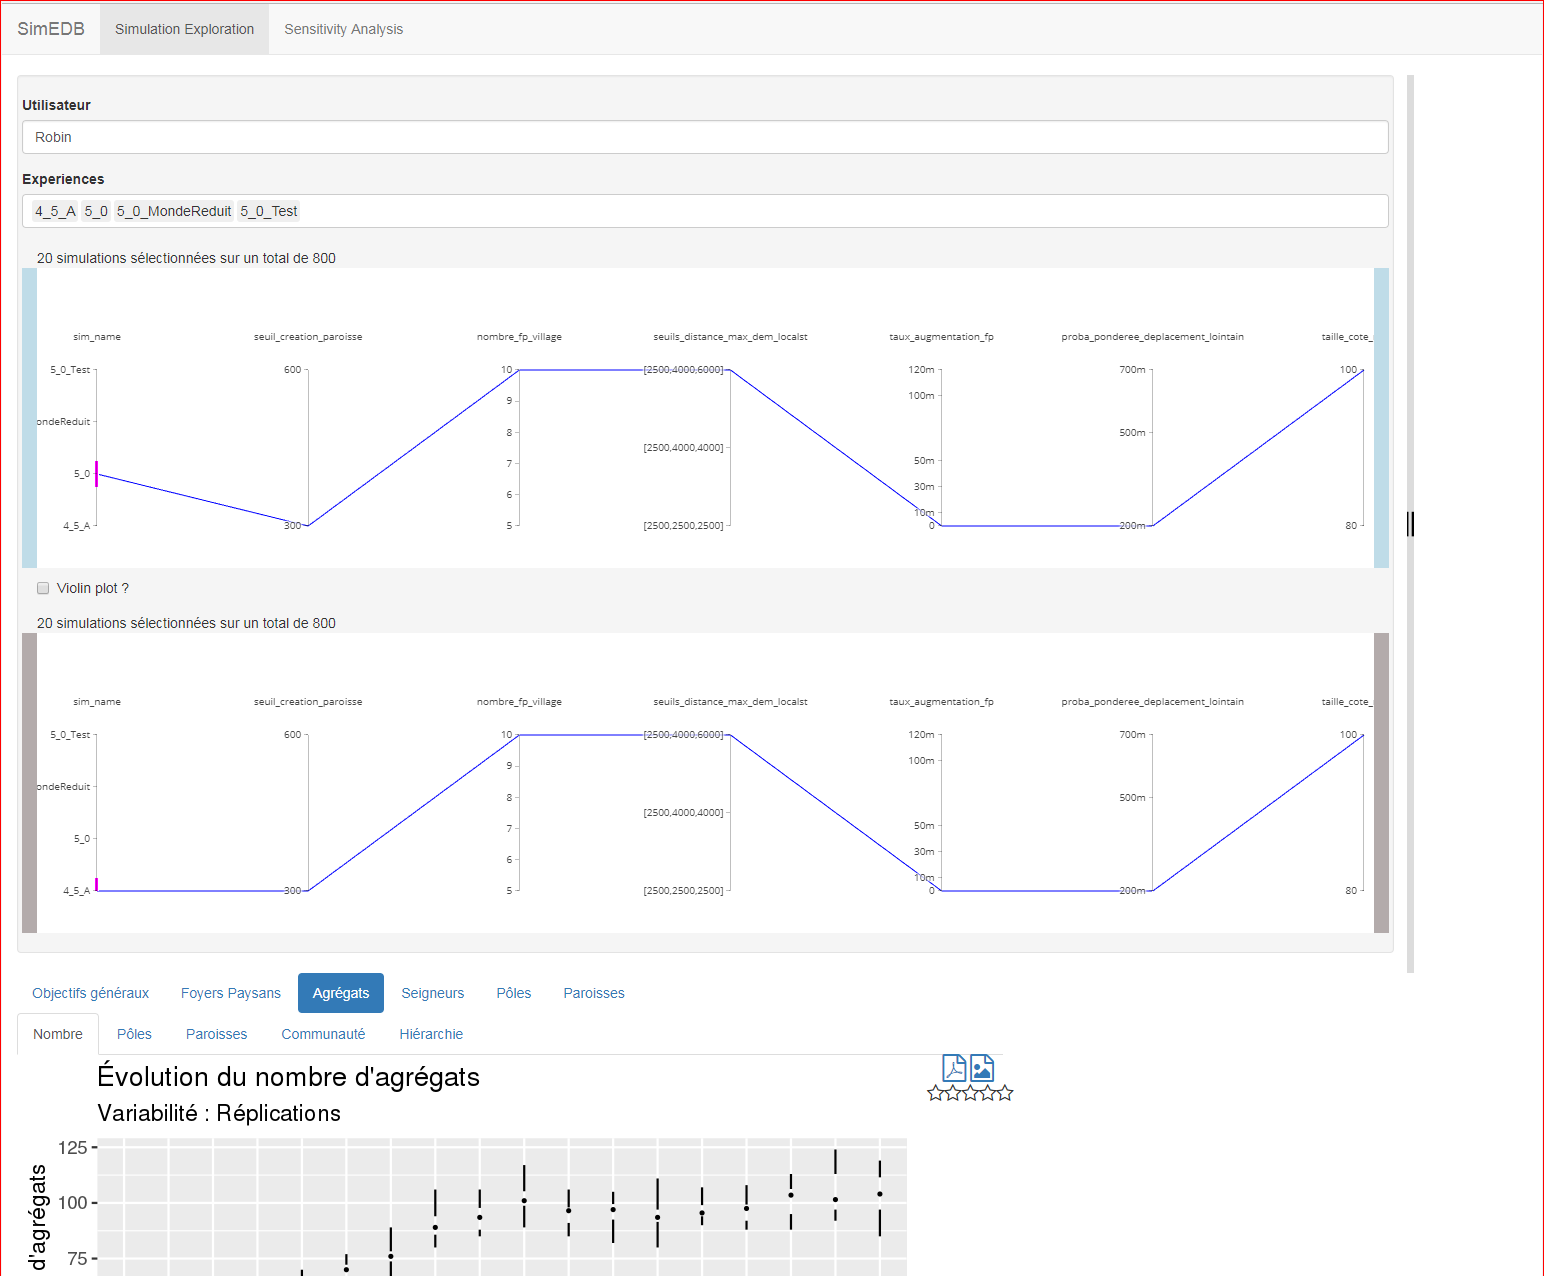
\includegraphics[width=\linewidth]{img/SimEDB_selection.png}
\end{minipage} \hfill
\begin{minipage}[b]{.49\linewidth}
\centering
\vspace{0pt}
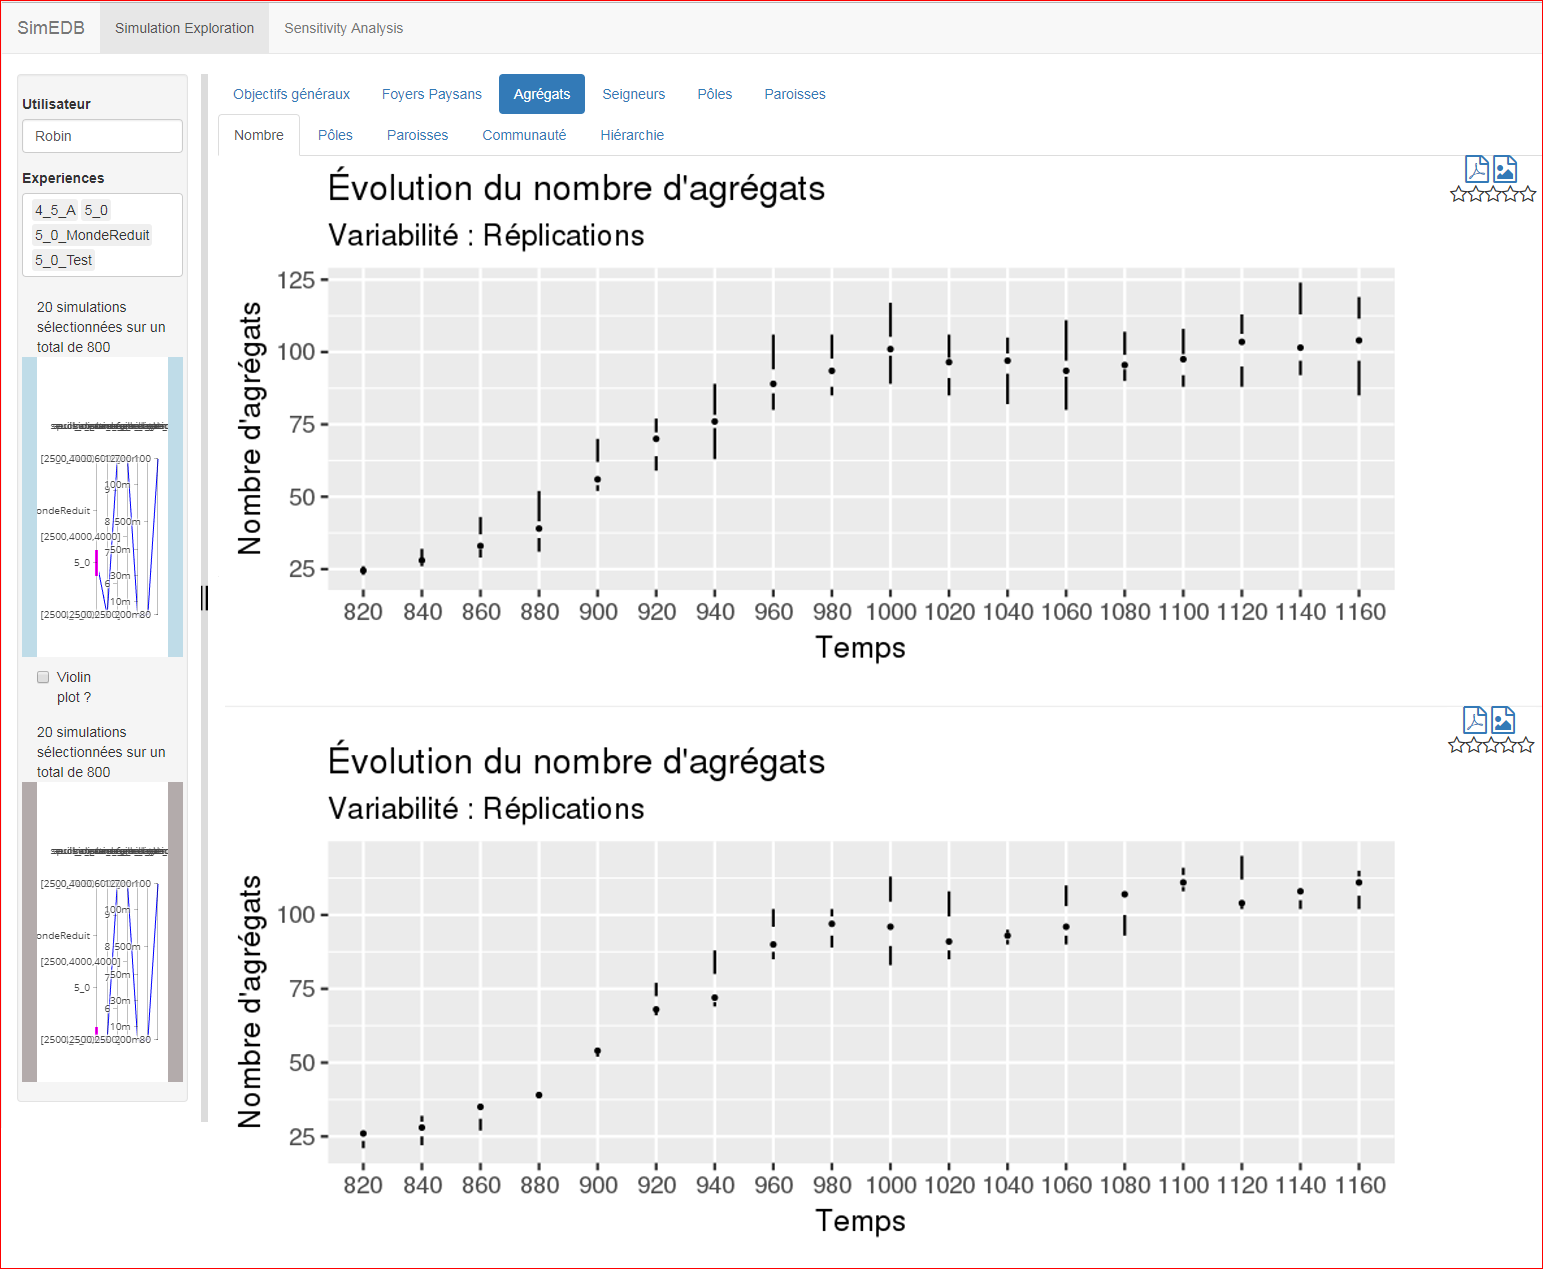
\includegraphics[width=\linewidth]{img/SimEDB_indicateur_grand_magnified.png}
\end{minipage}
\caption{Utilisation interactive de SimEDB et redimensionnement du panneau de contrôle.}
\label{fig:resizing}
\end{figure}

\paragraph*{Répondre aux demandes des utilisateurs : ajout d'un mécanisme d'export des indicateurs}

L'intérêt d'une interface modulaire et factorisée se révèle véritablement quand les utilisateurs d'un outil demandent des fonctionnalités supplémentaires, non prévues lors de la conception de l'outil.
Dans le cas de SimFeodal, une telle requête est rapidement apparue : les thématiciens, mais aussi les modélisateurs, pour conserver une trace d'une session d'exploration des indicateurs, souhaitaient pouvoir exporter les graphiques correspondant aux indicateurs.
Si au départ, une simple capture d'écran pouvait suffire, ce besoin a été complété par une volonté d'inclure des indicateurs de simulations dans des articles et autres communications, requérant donc des retouches des graphiques.
Pour ce faire, on a choisi d'ajouter des fonctionnalités de téléchargement des graphiques, selon deux formats -- image et vectoriel -- afin de satisfaire à ces deux usages.
Avec le développement modulaire adopté, il a suffit d'ajouter ces fonctions d'export en un unique lieu dans le code-source de SimEDB, et l'ajout de ces nouvelles fonctionnalités a alors été disponible automatiquement pour chacun des indicateurs graphiques.

\medskip
\hl{Ajouter un paragraphe, plus tard, sur l'inscription des modalités de filtrage (quelles sont les filtres appliqués ?) dans les graphiques, si j'arrive à trouver le temps de l'ajouter un jour...}

\paragraph*{Noter les simulations}

Un dernier point d'interaction avec l'application a été prévu, sans pouvoir toutefois être mobilisé jusque là : il s'agissait d'aller vers une semi-automatisation de l'évaluation des simulations, par l'intermédiaire d'un outil graphique permettant de \og noter\fg{} les simulations sélectionnées.
Pour ce faire, et parce que, on l'a vu, l'évaluation d'un ensemble de simulations ne peut se faire de manière unique, on a choisi de donner la possibilité aux utilisateurs experts de noter chacun des indicateurs de sortie, pour chacun des ensembles de simulations qu'ils exploreraient.
L'évaluation se fait au moyen d'un outil simple, composé de 5 \og étoiles\fg{}, et est enregistré à chaque nouvelle note.

Une piste d'utilisation serait de mobiliser les données ainsi créées, composées d'une note donnée à un indicateur pour un ensemble d'identifiants uniques de simulations, afin de réaliser des analyses quantitatives des notes attribuées : est-ce que certaines simulations sont systématiquement bien notées avec chacun des indicateurs affichés ? Certains indicateurs ne sont-ils jamais observés ou ne donnent-ils jamais lieu à évaluation ?

Cette fonctionnalité, bien qu'implémentée, n'est pas encore utilisée, mais devrait à terme permettre d'aller vers une meilleure connaissance des résultats de simulation, tout autant que vers une mesure de l'efficacité des indicateurs de sortie choisis pour évaluer un ensemble de simulations.

\subsubsection{Présentation générale}

\begin{itemize}
\item \hl{Quelques captures d'écran successives avec focus à chaque fois sur l'interaction en cours, ou alors,}
\item \hl{renvoyer à un manuel utilisateur en annexe, ou alors,}
\item \hl{ajouter un tuto interactif à l'application et en mettre le lien + descriptif ici}
\end{itemize}


%\setcounter{section}{4}
%\clearpage
\section*{Conclusion}
\addcontentsline{toc}{section}{\protect\numberline{}Conclusion}

\hl{A reprendre !}\\
% TODO : Reprendre conclusion
Au terme de la construction de la plate-forme d'exploration, nous disposons donc d'une application, SimEDB, conçue et développée spécifiquement pour les problématiques propres à l'exploration des données de SimFeodal.

Elle s'inscrit dans les méthodes des Interactions Homme-Machine, ou même dans ce que certains nomment désormais les \og Interactions Homme-Données\fg{} (\og \textit{Human-Data Interaction}\fg{}, \cite{elmqvist_embodied_2011,mortier_human-data_2014}) et s'efforce de suivre les préceptes identifiés dans ce champs (\cite[167-170]{amirpour_amraii_human-data_2018} par exemple).

Le développement a été fortement guidé par les contraintes et besoins identifiées, aussi bien en terme d'approches méthodologiques que de choix technologiques.
SimEDB est donc un outil \textit{ad-hoc}, toutefois pensé de manière modulaire.
Tous les composants logiciels de SimEDB sont indépendants et communiquent de manière standardisée, ouvrant la voie à leur remplacement ou \og interchangeabilité\fg{} : l'architecture logicielle et les choix techologiques le permettent.
La plate-forme SimEDB est donc intrinsèquement pensée comme une réponse à des besoins spécifiques, mais cette réponse a été conçue comme générique et en mesure d'être adaptée aisément à d'autres types de données et/ou sorties de modèles de simulation.

Plus généralement, l'ensemble de ce chapitre montre une démarche similaire, pensée pour répondre à des besoins spécifiques avec des solutions génériques et généralisables.
Le passage, depuis une succession de rapports jusqu'à une application d'exploration de ces rapports, ou encore les différents éléments relatifs au choix d'un système de gestion de base de données ou au dessin d'un modèle conceptuel de données s'inscrivent en effet dans cette même démarche qui s'ancre profondément dans une logique de recherche reproductible, aussi bien d'un point de vue technique que de celui du concept et de la méthodologie.


% Pour compilation finale, décommenter la dernière ligne :
% Permet d'enlever la page vide après le chapitre, mais bloque la création du minitoc. A faire donc après avoir recompilé une dernière fois avec le minitoc
%\let\clearpage\relax
% -> Remplacé pas l'usage de newclude::include*{}

\printbibliography[title={Références}]
